%\documentclass[a4paper, 14pt]{article}
\documentclass[14pt]{extarticle} % Note the extarticle document class

\usepackage[utf8]{inputenc}
\usepackage{graphicx}
\usepackage{float}%"Плавающие" картинки
\usepackage{wrapfig}%Обтекание фигур (таблиц, картинок и прочего)
\usepackage{amsmath, amssymb, amsthm}
\usepackage[T1, T2A]{fontenc}
\usepackage[english, russian]{babel}
\usepackage[left=2cm,right=2cm, top=2cm, bottom=2cm]{geometry}
% Литература в biblatex
\usepackage[backend=biber,bibencoding=utf8,language=auto,autolang=other,sorting=ntvy,babel=other,
            maxbibnames=99,maxcitenames=2,style=gost-numeric,movenames=false]{biblatex}
\addbibresource{../doc/refs.bib}
% Межстрочный интервал = 1.5pt
\usepackage{setspace}
\onehalfspacing
%\doublespacing
%\setstretch{1.5}
% % Абзацный отступ = 1.25см
\usepackage{indentfirst}
\setlength\parindent{12.5mm}
% Путь до папки с изображениями
\graphicspath{ {./images/} }
% Активные ссылки на формулы и лит-ру
\usepackage[
  colorlinks=true,
  citecolor=blue,
  linkcolor=blue,
  linktoc=page,
]{hyperref}
% cleverref
\usepackage{cleveref}
\newcommand{\crefrangeconjunction}{~--~}
\newcommand{\crefpairconjunction}{, }
\newcommand{\creflastconjunction}{, }
\crefname{equation}{}{}
% glossaries
\usepackage[automake,symbols,nogroupskip,sort=use]{glossaries-extra}
%\usepackage{array}
%\usepackage{booktabs}
% figures
\usepackage{subcaption}
% tilde symbol
\usepackage{textcomp}
\renewcommand{\texttilde}{\raisebox{0.5ex}{\texttildelow}}
% Reynolds number
\newcommand{\Ren}{\mathrm{Re}}
\renewcommand{\vec}[1]{\boldsymbol{\rm #1}}
%dx, dy
\newcommand{\dx}{\triangle x}
\newcommand{\dt}{\triangle t}
\newcommand{\CFL}{\mathrm{CFL}}
% 
\newcommand{\dfr}[2]{\frac{\partial #1}{\partial #2}}
\newcommand{\dfrq}[2]{\frac{\partial^2 #1}{\partial #2^2}}
\newcommand{\dsfr}[2]{\left.\partial #1\middle/\partial#2\right.}

\makeglossaries

\begin{document}

\begin{titlepage}
\begin{center}

\hfill \break

\large{Министерство науки и высшего образования Российской~Федерации}\\
\footnotesize{Федеральное государственное автономное образовательное учреждение высшего образования}\\ 
\small{\textbf{«КАЗАНСКИЙ (ПРИВОЛЖСКИЙ) ФЕДЕРАЛЬНЫЙ УНИВЕРСИТЕТ»}}\\

\hfill \break
\normalsize{Институт механики и математики им. Н. И. Лобачевского}\\

\hfill \break
\normalsize{Направление подготовки: 01.01.03 Механика и математическое моделирование}\\

\vspace{25mm}
\large{Курсовая работа}\\
\end{center}

\vspace{20mm}
\noindent
Студентка 3 курса \\
группы 05-001 \\
<<\underline{\hspace{0,75cm}}>> \underline{\hspace{2cm}}\the\year~г.

\hfill \break
Научный руководитель \\
<<\underline{\hspace{0,75cm}}>>\underline{\hspace{2cm}}\the\year~г.

\vspace{\fill}

\begin{center}
    Казань, \the\year
\end{center}
\thispagestyle{empty}

\end{titlepage}


\newpage
\tableofcontents
\newpage

\section{Введение}
\subsection{Актуальность работы}

Кровь -- соединительная ткань внутри организма, она состоит из форменных клеток (эритроцитов, лейкоцитов, тромбоцитов), а так же из
водного раствора белков и свёртывающих веществ -- плазмы. Кровь под воздействием периодических сокращений сердечной мышцы 
движется по замкнутой системе сосудов, циркулируя от сердца и обратно. С точки зрения гидродинамики кровоток представляет 
из себя пульсирующее с низкой частотой течение мелкодисперсной суспензии в 
замкнутой системе каналов кругового сечения с эластичными стенками, осложнённое локальными эффектами ламинарно-турбулентного перехода.

Сложность разветвления кровеносных сосудов и вариации их размеров создают значительные трудности при решении задачи о течении крови. 
Математическое моделирование помогает  
аппроксимации и пониманию сложностей кровотока. Эти модели позволяют описывать и строить физические процессы, происходящие 
в биологических областях, что может быть полезно при выявлении, прогрессировании и лечении  различных сердечно-сосудистых заболеваний , 
а так же в проектировании и оптимизации медицинских устройств.

Описывать кровь можно различными способами. Например, детально: кровь состоит из взвешенных в плазме 
(которую чаще рассматривают, как ньютоновскую жидкость) клеток крови, которые действуют друг на друга с некоторыми силами. 
Описание такого типа методов можно подробнее изучить в ~\cite{Fedosov:2010,Fedosov:2008,Mehboudi:2001}. 
В некоторых моделях ~\cite{bessonov:2014,hosseini:2009} пренебрегают относительно мелкими и редкими -- тромбоцитами
(2--4~мкм в количестве 150--300 миллионов на 1~см$^3$) и лейкоцитами(4--20~мкм в количестве 4.5 -- 11 миллионов на 1~см$^3$), 
а строят двумерные сетки, состоящие только лишь из эритроцитов (7 -- 8~мкм в количестве 3.8 до 5.6 миллиардов клеток на 1~см$^3$).
Но при таких подходах можно столкнуться с некоторыми проблемами: такую модель будет сложно сравнивать как
с другими моделями, так и с эксперементальными показателями, так же она очень плохо реагирует на любые изменения в исходных данных. 
Соответсвенно, возникает необходимость прибегнуть к дальнейшему осреднению.

Можно не описывать индивидуальные частицы взвешенные в плазме, а обобщить их до вязкой неньютоновской жидкости с определёнными 
характеристиками, тогда любые изменения можно будет отразить в параметрах жидкости. Такой подход называют трехмерным моделированием.
Существует множество трёхмерных моделей, например, основанные на зависимости вязкости от гематокрита ~\cite{walburn:1976},
модель Максвелла \cite{thurston:1972},  модель Кассона ~\cite{moller:2006}.
Однако эти модели всё-таки требуют значительных вычислительных ресурсов, а следовательно, и дальнейших упрощений. 

Для вывода граничных условий в трёхмерных моделях иногда используют одномерное моделирование, которое может быть 
и вполне самостоятельным подходом к моделированию течения крови.
В одномерных моделях пространственные характеристики осредняются по поперечному сечению, а трёхмерная дифференциальная
задача сводится к одномерной. Такой подход к моделированию требует меньших вычислительных ресурсов, но при этом почти не уступает в 
точности другим моделям. О сравнении одномерных и многомерных моделей можно прочитать в ~\cite{FORMAGGIA:2001}.

В постановке задачи одномерного моделирования есть несколько ключевых аспектов. Первое -- 
определение геометрии сосудов: их длина, поперечное сечение, разветвлённость. Точность определения этих данных существенно влияет 
на результат моделирования. Для повышения точности геометрических данных сравнивают данные из различных
источников, используют МРТ и ультразвуковые исследования, а так же калибруют уже готовую модели. В работе 
\cite{Shanmugavelayudam:2010} рассматривают влияние геометрических допущений на численное моделирование.

Так же необходимо задать физические характеристики крови, такие как её плотность (обычно её оценивают в 1052 -- 1060~кг/м\textsuperscript{3}),
вязкость (4.3 -- 4.9~мПа$\cdot$с), состав крови (количество эритроцитов, лейкоцитов и тромбоцитов, увеличение или уменьшение ктороых
влияет и на другие физические характеристики. Подробнее в~\cite{Bouchnita2020}).

Кровь, двигаясь по сосудам, испытывает сопротивление движению со стороны сосудов и из-за своей вязкости. Поэтому сердце вбрасывает 
кровь в сосуды под большим давлением. В аорте давление колеблется в диапазоне от 120~мм рт.ст. при систоле до 80~мм рт.ст. при диастоле. 
По мере движения крови давление в сосудистом русле падает. 

Скорость течения крови так же зависит от диаметра сосуда, удалённости сосуда от сердца, а также фазы сердечного цикла. 
Максимальных значений скорость достигает в аорте (до \texttilde$1$~м/с), а минимальных -- в капиллярах (около нуля).
Линейная скорость в полых венах в два раза меньше, чем в аорте и равна примерно $2.5\cdot10^{-1}$~м/с, 
поскольку в организме на одну артерию приходится две вены.

Необходимо так же определиться и с граничными условиями. В общем случае: на входе задаётся  систолическое давление, 
а на выходе диастолическое. О влиянии граничных условий в задаче одномерного моделирования можно прочитать в~\cite{Krivovichev:2022}.

Для построения модели нужно выбрать подходящий метод. Метод конечных элементов~\cite{TAYLOR1998} -- популярная численная схема. 
Он особенно хорошо подходит для моделирования сложных геометрий, таких как запутанная сеть артерий в человеческом теле. 
Однако он может быть вычислительно дорогим, особенно для больших и сильно разветвленных сетей. 

Метод быстрого преобразования Фурье~\cite{Sazonov:2019} -- 
это подход, использующий быстрое преобразование Фурье для решения одномерных уравнений кровотока. 
Этот метод конкурирует с традиционными пространственно-временными численными схемами как по устойчивости, так и по скорости. 
Он может точно и эффективно обрабатывать сложные геометрические формы и высокоамплитудные волны. 
Однако он требует дальнейшего развития для учета вязкоупругих эффектов и потери массы крови из-за мелких ветвей. 

Метод прерывистого Галеркина~\cite{yao:2017} -- это еще одна численная схема, она сочетает в себе преимущества методов конечной разности и конечных элементов, 
обеспечивая баланс между точностью и вычислительными затратами. Однако он может быть более сложным в реализации и может
потребовать дополнительных вычислительных ресурсов для сопоставления расчетной и физической областей.

Метод конечных объемов с локальным временным шагом высокого порядка~\cite{mueller:2015} предполагает решение управляющих уравнений 
с помощью метода конечных объемов высокого порядка и схемы локального шага по времени. 
Этот метод может быть особенно полезен для моделирования течения в сложных геометрических системах.

Метод конечных разностей предполагает дискретизацию области на сетку точек и последующую аппроксимацию производных в управляющих
уравнениях с помощью конечных разностей. Этот метод часто используется в сочетании со схемой интегрирования по времени для решения 
полученной системы обыкновенных дифференциальных уравнений.



\section{Постановка задачи}

\glsxtrnewsymbol[description={пространственная координата вдоль сосуда, [м]}]{x}{\ensuremath{x}}
\glsxtrnewsymbol[description={время, [с]}]{t}{\ensuremath{t}}
\glsxtrnewsymbol[description={площадь поперечного сечения сосуда в фиксированном сечении, [м\textsuperscript{2}]}]{a}{\ensuremath{a}}
\glsxtrnewsymbol[description={$=\sqrt{a/\pi}$, радиус сосуда, [м]}]{R}{\ensuremath{R}}
\glsxtrnewsymbol[description={средняя по поперечному сечению сосуда скорость жидкости, [м/с]}]{u}{\ensuremath{u}}
\glsxtrnewsymbol[description={среднее по поперечному сечению сосуда давление, [Па]}]{p}{\ensuremath{p}}
\glsxtrnewsymbol[description={плотность жидкости, [кг/м\textsuperscript{3}]}]{rho}{\ensuremath{\rho}}
\glsxtrnewsymbol[description={динамическая вязкость жидкость, [Па$\cdot$c]}]{mu}{\ensuremath{\mu}}
\glsxtrnewsymbol[description={нормированная на общий радиус $R$ радиальная координата сосуда, [1]}]{r_prime}{\ensuremath{r'}}
\glsxtrnewsymbol[description={нормированный профиль скорости, [1]}]{U}{\ensuremath{U}}
\glsxtrnewsymbol[description={параметр, описывающий радиально-симметричный профиль скорости, [1]}]{zeta}{\ensuremath{\zeta}}
\glsxtrnewsymbol[description={параметр, описывающий эластичные свойства материала стенки сосуда, [кг/с\textsuperscript{2}]}]{beta}{\ensuremath{\beta}}
\glsxtrnewsymbol[description={модуль упругости стенки сосуда, [Па]}]{E}{\ensuremath{E}}
\glsxtrnewsymbol[description={толщина стенки сосуда, [м]}]{h}{\ensuremath{h}}
\glsxtrnewsymbol[description={площадь поперечного сечения сосуда при отсутствии внешнего воздействия, [м\textsuperscript{2}]}]{A}{\ensuremath{A}}
\glsxtrnewsymbol[description={объёмный расход жидкости, [м\textsuperscript{3}/с]}]{q}{\ensuremath{q}}
\glsxtrnewsymbol[description={коэффициент при вязком слагаемом в определяющей системе уравнений, [м\textsuperscript{2}/с]}]{Knu}{\ensuremath{K_{\nu}}}
\glsxtrnewsymbol[description={переменные Римана, [м/с]}]{w12}{\ensuremath{w_{1,2}}}
\glsxtrnewsymbol[description={скорости переноса переменных Римана, [м/с]}]{lambda12}{\ensuremath{\lambda_{1,2}}}
\glsxtrnewsymbol[description={скорость переноса возмущений, [м/с]}]{c}{\ensuremath{c}}
\glsxtrnewsymbol[description={$=c(A)$, скорость переноса возмущений в нейтральном состоянии сосуда, [м/с]}]{c0}{\ensuremath{c_0}}
\glsxtrnewsymbol[description={полное давление[Па]}]{P}{\ensuremath{P}}

\subsection{Определяющая система уравнений}
Для выводы определяющей системы уравнений будем следовать подходу~\cite{Hughes1973}
с некоторыми упрощениями.

\subsubsection{Осреднение по сечению сосуда}

\begin{figure}[h]
    \centering
    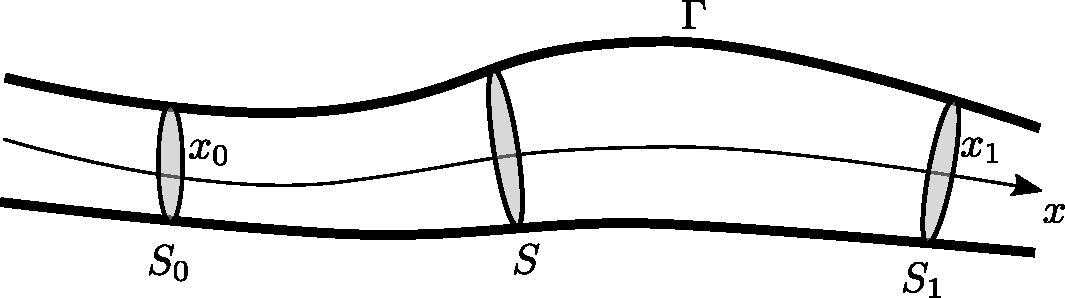
\includegraphics[width=0.6\linewidth]{def.pdf}
    \caption{Элементарный объём $V$}
    \label{fig:elementary_volume}
\end{figure}

Будем рассматривать течение в сосуде с продольной координатой \gls{x}.
Определим элементарный объём $V$ как отрезок сосуда при $x\in[x_0, x_1]$ (см. рис.~\ref{fig:elementary_volume}).
Границей этого объема будут входное и выходное сечения $S_0$, $S_1$ и
боковая граница $\Gamma$: $\partial V = S_0 \cup S_1 \cup \Gamma$.

Пусть величина $g$ переносится в этом элементарном объёме несжимаемой
жидкостью со скоростью $\vec u$:
\begin{equation}
\label{eq:divu}
\nabla\cdot \vec u = 0.
\end{equation}
Тогда распишем изменения по времени \gls{t}  интеграла от этой величины $g$ согласно теореме Рейнольдса:
\begin{equation}
\label{eq:reynolds-transport}
\frac{d}{dt}\int\limits_{V}g\,d\vec x = 
\int\limits_{V}\dfr{g}{t}\,d\vec x + \int\limits_{\partial V} g v_n \,d s
\end{equation}
Здесь $v_n$ -- нормальная скорость объема $V$.
Будем считать, что объём не совершает продольного движения. То есть
\begin{equation}
\label{eq:zero_vn}
\left.v_n\right|_{S_0, S_1} = 0.
\end{equation}
Определим среднее по сечению значение как
\begin{equation}
\label{eq:average_g}
\bar g = \frac{1}{|S|}\int\limits_S g \, ds.
\end{equation}
Тогда, с учётом того, что координаты $x_0$, $x_1$ не зависят
от времени (как следствие из \cref{eq:zero_vn}), левая часть \cref{eq:reynolds-transport} может быть представлена
в виде
\begin{equation}
\label{eq:left_in_reynolds_transport}
\frac{d}{dt}\int\limits_{V}g\,d\vec x = 
\int\limits_{x_0}^{x_1} \dfr{|S| \bar g}{t} \, dx.
\end{equation}

Далее рассмотрим второе слагаемое в правой части \cref{eq:reynolds-transport}.
Обозначим за $w_n$ -- скорость объема относительно $u_n$ -- скорости жидкости:
\begin{equation}
\label{eq:wn_vn_un}
w_n = v_n - u_n.
\end{equation}
\begin{equation}
\label{eq:second_in_reynolds_transport}
\int\limits_{\partial V} v_n g \, ds = 
\int\limits_{\partial V} w_n g \, ds +
\int\limits_{\partial V} u_n g \, ds.
\end{equation}
Для первого слагаемого в правой части \cref{eq:second_in_reynolds_transport} справедливо

\begin{align*}
\int\limits_{\partial V} w_n g \, ds
	& = \int\limits_{\Gamma} w_n g \, ds
	  + \int\limits_{S_0} w_n g \, ds
	  + \int\limits_{S_1} w_n g \, ds = \dots \\
\intertext{расписывая $w_n$ по \cref{eq:wn_vn_un} с учётом \cref{eq:zero_vn}}
	& = \int\limits_{\Gamma} w_n g \, ds
	  - \int\limits_{S_0} u_n g \, ds
	  - \int\limits_{S_1} u_n g \, ds = \dots \\
\intertext{подставляя определение \cref{eq:average_g} для произведения $u_n g$}
	& = \int\limits_{\Gamma} w_n g \, ds
	  - \left(|S|\overline{u_n g}\right)_{x_0}
	  - \left(|S|\overline{u_n g}\right)_{x_1} = \dots \\
\intertext{заменим нормальную скорость $u_n$ скоростью $u_x$ по направлению координаты $x$ с учётом направления внешней нормали в сечениях $x_0$, $x_1$}
	& = \int\limits_{\Gamma} w_n g \, ds
	  + \left(|S|\overline{u_x g}\right)_{x_0}
	  - \left(|S|\overline{u_x g}\right)_{x_1} = \dots\\
\intertext{применяя формулу интегрирования по частям}
	& = \int\limits_{\Gamma} w_n g \, ds
	  - \int\limits_{x_0}^{x_1} \dfr{|S| \overline{u_x g} }{x} \, dx.
\end{align*}

Второе слагаемое в правой части \cref{eq:second_in_reynolds_transport} распишем по формуле Гаусса-Остроградского
с учётом условия неразрывности \cref{eq:divu}:
\begin{equation}
\nonumber
\int\limits_{\partial V} u_n g \, ds =
\int\limits_{V} \vec u \cdot \nabla g \, d\vec x
\end{equation}

Собирая равенство \cref{eq:reynolds-transport} с учётом полученных соотношений получим
\begin{equation}
\nonumber
\int\limits_{x_0}^{x_1} \left( \dfr{|S| \bar g}{t} + \dfr{|S| \overline{u_x g} }{x}\right) \, dx =
\int\limits_V \left(\dfr{g}{t} + \vec u \cdot \nabla g \right)\, d\vec x
+ \int\limits_{\Gamma} w_n g \, ds
\end{equation}
Далее, пользуясь произвольностью выбора продольной координаты снимем интегрирование по $x$:
\begin{equation}
\label{eq:common_s_average}
\dfr{|S| \bar g}{t} + \dfr{|S| \overline{u_x g} }{x} =
\int\limits_{S(x)} \left(\dfr{g}{t} + \vec u \cdot \nabla g \right)\, ds
+ \oint\limits_{L(x)} w_n g \, dl.
\end{equation}
Здесь $L$ -- сечение поверхности $\Gamma$ по фиксированной продольной координате $x$.

\subsubsection{Сохранение массы}
Для получения закона сохранения массы рассмотрим общее
соотношение \cref{eq:common_s_average} при $g = 1$:
\begin{equation}
\nonumber
\dfr{|S|}{t} + \dfr{|S| \overline{u_x} }{x} =
\oint\limits_{L(x)} w_n \, dl.
\end{equation}
Интеграл в правой части -- есть расход жидкости через 
боковые стенки сосуда. В настоящей работе мы ограничимся
случаем непроницаемых стенок сосуда:
\begin{equation}
\nonumber
\left.w_n \right|_\Gamma = 0,
\end{equation}
Тогда этот интеграл будет равен нулю.
Для величин в левой части введём обозначения:
$\gls{a} = |S|$ -- площадь поперечного сечения сосуда, равная $a = \pi \gls{R}^2$.
$\gls{u} = \bar u_x$ -- средняя по сечению продольная скорость жидкости.
Тогда закон сохранения масс примет вид
\begin{equation}
\label{eq:mass_conservation}
\dfr{a}{t} + \dfr{u a}{x} =0
\end{equation}

\subsubsection{Сохранение количества движения}
Рассмотрим уравнения \cref{eq:common_s_average}
при $g = u_x$. С учётом введённых обозначений получим
\begin{equation}
\label{eq:momentum_first}
\dfr{a u}{t} + \dfr{a \bar u_x^2 }{x} =
\int\limits_{S(x)} \left(\dfr{u_x}{t} + \vec u \cdot \nabla u_x \right)\, ds
+ \oint\limits_{L(x)} w_n u_x \, dl.
\end{equation}

Для последующих выкладок сделаем допущение, что форма профиля скорости вдоль всей длины сосуда постоянна (не зависит от координаты $x$)
и радиально-симметрична (зависит только от нормированной радиальной координаты $\gls{r_prime} = r/R$).
То есть $u_x$ представима в виде
\begin{equation}
\label{eq:ux_simplification}
u_x(x, s) = u(x) U(r'),
\end{equation}
где \gls{U} -- нормированный профиль скорости.

Правую часть распишем с использованием ранее выведенного закона сохранения масс \cref{eq:mass_conservation}:
\begin{align}
\dfr{a u}{t} + \dfr{a \bar u_x^2 }{x}
   & = a\dfr{u}{t} - u\dfr{au}{x} + \dfr{a \bar u_x^2 }{x} = \dots\nonumber\\
\intertext{добавим и вычтем слагаемое $\dsfr{au^2}{x}$}
   & = a\dfr{u}{t} - u\dfr{au}{x} + \dfr{au^2}{x} + \dfr{a (\bar u_x^2 - u^2)}{x} = \dots\nonumber\\
\intertext{разложим третье слагаемое и проведём сокращения}
   & = a\dfr{u}{t} + au\dfr{u}{x} + \dfr{a (\bar u_x^2 - u^2)}{x} = \dots\nonumber \\
\intertext{воспользуемся упрощением \cref{eq:ux_simplification}}
   & = a\dfr{u}{t} + au\dfr{u}{x} + (\bar U^2 - 1)\dfr{a u^2}{x}\label{eq:momentum_first_left}.
\end{align}

Упрощение первого интеграла в правой части будем проводить на
основе общего уравнения движения для вязкой несжимаемой жидкости, записанного в проекции на ось $x$:
\begin{equation}
\label{eq:ns_ux}
\dfr{u_x}{t} + \vec u \cdot \nabla u_x = -\frac{1}{\rho} \dfr{p}{x} + \frac{\mu}{\rho}\nabla^2 u_x,
\end{equation}
где \gls{p} -- давление, \gls{rho} -- плотность и \gls{mu} -- вязкость жидкости.
Будем считать,
что продольные изменения скорости намного меньше, чем поперечные. Это справедливо, если справедливы условия
прилипания к боковым стенкам канала. Тогда можно записать
\begin{equation}
\nonumber
\nabla^2 u_x = \nabla^2_S u_x + \dfrq{u_x}{x} \approx \nabla^2_S u_x,
\end{equation}
за $\nabla^2_S$ обозначен двумерный оператор Лапласа, действующий в плоскости $S$.
Подставим это приближение в выражение \cref{eq:ns_ux} 
и проинтегрируем по плоскости $S$:
\begin{align}
\int\limits_S\left(\dfr{u_x}{t} + \vec u \cdot \nabla u_x\right)\, ds
	& = -\frac{1}{\rho} \int\limits_S\dfr{p}{x}\, ds + \frac{\mu}{\rho}\int\limits_S\nabla^2_S u_x \, ds = \dots\nonumber\\
\intertext{будем считать, что давление слабо меняется поперёк канала: $p(x, s)\approx\bar p(x)$}
	& = -\frac{1}{\rho} |S|\dfr{p}{x} + \frac{\mu}{\rho}\int\limits_S\nabla^2_S u_x \, ds = \dots\nonumber\\
\intertext{и раскроем второй интеграл с помощью интегрирования по частям}
	& = -\frac{1}{\rho} |S|\dfr{p}{x} + \frac{\mu}{\rho}\oint\limits_L \dfr{u_x}{n_l} \, dl = \dots\nonumber\\
\intertext{в радиально-симметричном упрощении, при котором $n_l = r$}
	& = -\frac{1}{\rho} |S|\dfr{p}{x} + \left.\frac{2\pi\mu R}{\rho}\dfr{u_x}{r}\right|_{r=R(x)} = \dots\nonumber\\
\intertext{воспользуемся упрощением \cref{eq:ux_simplification} для вычисления последней производной}
	& = -\frac{1}{\rho} |S|\dfr{p}{x} + \left.\frac{2\pi \mu}{\rho} u \dfr{U}{r'}\right|_{r'=1} \label{eq:momentum_first_right}
\end{align}

Запишем уравнение \cref{eq:momentum_first} с учётом \cref{eq:momentum_first_left,eq:momentum_first_right}:
\begin{equation}
\label{eq:momentum_second}
\dfr{u}{t} + u\dfr{u}{x} + \frac{\bar U^2 - 1}{a}\dfr{a u^2}{x} =
	-\frac{1}{\rho} \dfr{p}{x} + \left.\frac{2\pi\mu}{\rho}\frac{u}{a}\dfr{U}{r'}\right|_{r'=1}.
\end{equation}

Для проведения дальнейших упрощений необходимо допущение о форме профиля $U$.
В простейшем случае можно считать его постоянным: $U=1$. Тогда
выражение \cref{eq:momentum_second} преобразуется к виду
\begin{equation}
\label{eq:momentum_conservation_inviscid}
\dfr{u}{t} + u\dfr{u}{x} = -\frac{1}{\rho} \dfr{p}{x}.
\end{equation}
Таким образом, мы получили уравнение движения при полном пренебрежении
силами вязкого трения о стенки сосуда.

\subsubsection{Учёт вязкого трения}
Рассмотрим радиальный профиль скорости \gls{U}, который задаётся параметрическим (зависящим от параметра $\zeta$) соотношением (см.~\cite{Hughes1973,Smith2001})
\begin{equation}
U_0(r') = \frac{\zeta+2}{\zeta} \left(1 - \left(r'\right)^{\zeta}\right).
\end{equation}
Случай $\zeta=2$ соответствует установившемуся профилю Пуазейля.
Более высокие значение $\zeta$ отражают неустановившийся характер течения.
Профили для некоторых $\zeta$ представлены на рис.~\ref{fig:U}.


\begin{figure}[h]
    \centering
    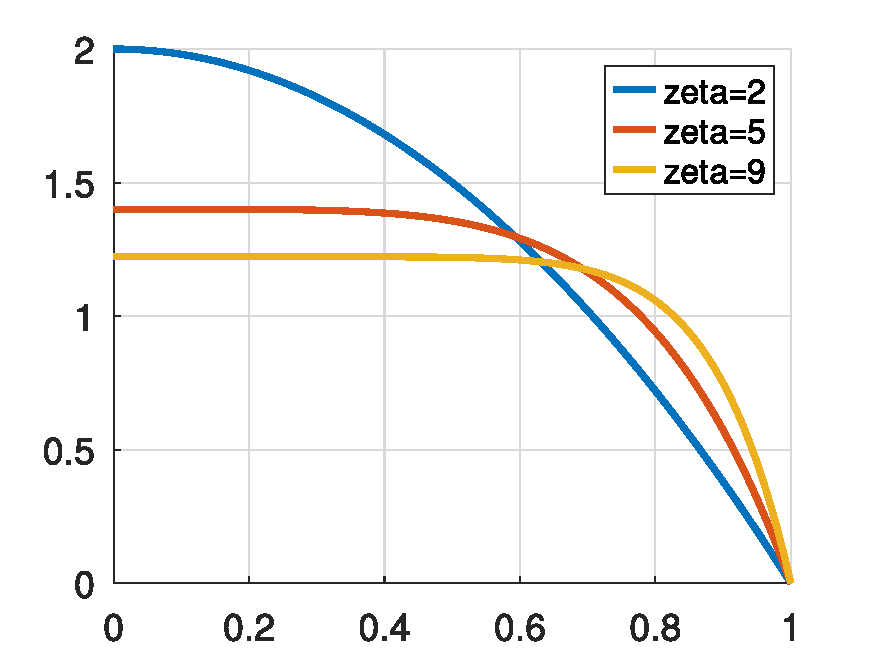
\includegraphics[width=0.4\linewidth]{U.pdf}
    \caption{Нормированный профиль скорости в зависимости от $\zeta$}
    \label{fig:U}
\end{figure}

Выражения из \cref{eq:momentum_second}, содержащие нормированную скорость, будут равны:
\begin{align*}
\left.\dfr{U}{r'}\right|_{r'=1} &= - (\zeta+2),\\
\bar U &= 1,
\end{align*}
тогда само уравнение сохранения количества движения примет вид
\begin{equation}
\label{eq:momentum_conservation_viscous}
\dfr{u}{t} + u\dfr{u}{x} =
	-\frac{1}{\rho} \dfr{p}{x} - K_{\nu}\frac{u}{a},
\end{equation}
где влияние вязкости описывается коэффициентом
\begin{equation}
\nonumber
\gls{Knu} = \frac{2\pi\mu(\zeta+2)}{\rho}.
\end{equation}

\subsubsection{Замыкающее соотношение для давления}
Постановка задачи включает в себя два уравнения \cref{eq:mass_conservation,eq:momentum_conservation_viscous}
для трёх неизвестных $u$, $a$, $p$. Таким образом, необходимо ещё одно,
замыкающее соотношение.
Обычно таким соотношением служит зависимость давления от площади поперечного сечения $p(a)$.
Следуя~\cite{Formaggia2003} запишем эту зависимость в приближении равновесного состояния (давление мгновенно подстраивается под изменение площади сечения сосуда)
при условии нулевого внешнего давления:
\begin{equation}
\label{eq:p_from_a}
p(a) = \frac{\beta}{A} \left(\sqrt{a} - \sqrt A\right).
\end{equation}
Здесь \gls{A} -- нейтральный радиус сосуда,
а коэффициент \gls{beta} вычисляется в приближении тонкой, несжимаемой, однородной, изотропной, эластичной мембраны с толщиной \gls{h} и 
модулем упругости \gls{E}:
\begin{equation}
\nonumber
\beta = \frac{4}{3}\sqrt{\pi}E h.
\end{equation}

\subsection{Характеристический анализ}
Запишем полученную систему гиперболических уравнений \cref{eq:mass_conservation,eq:momentum_conservation_viscous}
в векторном виде:
\begin{equation}
\label{eq:vector_system}
\dfr{\vec U}{t} + \nabla \vec F(\vec U) = \vec B,
\end{equation}
где введены вектора:
\begin{equation}
\nonumber
\vec U =
\left(\begin{array}{c}
a \\
u
\end{array}\right),
\quad
\vec F(\vec U) =
\left(\begin{array}{c}
au\\
\dfrac{u^2}{2} + \dfrac{p}{\rho}
\end{array}\right),
\quad
\vec B =
\left(\begin{array}{c}
0\\
-K_{\nu} \dfrac{u}{a}
\end{array}\right).
\end{equation}
Такая система может быть приведена к характеристическому виду (см. например~\cite{Sherwin2003})
\begin{equation}
\label{eq:w12_system}
\begin{aligned}
&\dfr{w_1}{t} + \lambda_1 \dfr{w_1}{x} = 0, \\
&\dfr{w_2}{t} + \lambda_2 \dfr{w_2}{x} = 0.
\end{aligned}
\end{equation}
Правая часть здесь получена при условии $\mu=0$.
\gls{w12} -- переменные Римана, а \gls{lambda12} -- скорость переноса этих переменных, которые определены как
\begin{equation}
\label{eq:w12_def}
w_{1,2} = u \pm 4(c - c_0), \quad \lambda_{1,2} = u \pm c.
\end{equation}
через скорость переноса возмущений $\gls{c}(a)$:
\begin{equation}
\label{eq:c_from_a}
c = \sqrt{\frac12\frac{\beta}{A\rho}}a^{\frac{1}{4}}.
\end{equation}
Эта скорость зависит от площади сечения сосуда (чем сосуд более растянут, тем эта скорость больше).
Значение скорости в начальный момент определено как $\gls{c0} = c(A)$.
Отметим, что по построению значения $w_{1,2}$ равны нулю в состоянии покоя при $a=A$, $u=0$.
Этот факт будет использован при постановке граничных условий.

В рассматриваемой здесь задаче кровотока характерные
скорости течения крови не превышают 1 м/с в самых крупных сосудах,
а скорости распространения возмущений имеют на порядок большие характерные значения, то $c \gg u$,
значит
\begin{equation}
\nonumber
\lambda_1 > 0, \quad \lambda_2 < 0.
\end{equation}
Из этого можно сделать вывод, что
переменные Римана $w_1$  и $w_2$ строго однонаправлены и распространяются в противоположенные по отношению друг к другу стороны.
Для иллюстрации этого эффекта смотри тестовую задачу из пункта~\ref{sec:problem4}.

Зависимоть естественных переменных от переменных Римана запишется как
\begin{equation}
\label{eq:ua_from_w}
u = \frac{w_1 + w_2}{2}, \quad
a = \left(\frac{w_1 - w_2}{8} + c_0\right)^{4} \left(\frac{2\rho A}{\beta}\right)^2.
\end{equation}
То есть естественные переменные содержат комбинацию однонаправленных переменных. Отсюда
можно сделать вывод, что возмущения по естественным переменным могут распространяться
в обе стороны расчётной области. Этот факт следует иметь ввиду при формулировке граничных условий.

\subsection{Граничные условия и условия на разрывах}
Поскольку процесс описывается гиперболической системой из двух уравнений \cref{eq:w12_system},
то он требует задания граничного условия на тех границах,
на которых скорость распространения искомых величин противоположна внешней к границе нормали.
Переменные $w_1$ и $w_2$ распространяются в противоположенные стороны, то есть
на границе следует задавать только одну из этих переменных.
Для условности будем считать границы, на которых требуется задания $w_1$ входными,
а остальные -- выходными.

\subsubsection{Выходное условие}
На выходной границе поставим требования беспрепятственного выхода через границу.
То есть на ней не должно формироваться никаких возмущений. На практике это означает задание
\begin{equation}
\label{eq:outflow_w2}
\left.w_2\right|_{out} = 0.
\end{equation}

\subsubsection{Входное условие}
Во входном сечении сетки сосудов обычно задают либо входной профиль давления $p_{in}(t)$
либо общий расход $\gls{q}_{in}(t)$. Чтобы свести
эти физичные условия к условиям на переменные Римана также зададим требование неотражаемости входной границе.
Подобно тому, как на выходной границе мы требовали, чтобы приходящее возмущение от $w_1$ не
провоцировало исходящие возмущение $w_2$, так и на входной границе потребуем, чтобы
приходящее возмущение от $w_2$ не провоцировало возмущений для $w_1$.
При этом, в отличии от выходной границе, мы не можем просто занулить $w_1$;
возмущения в $w_1$ должны генерироваться за счёт физичных граничных условий -- $q_{in}$ либо $p_{in}$.
Таким образом, для постановки неотражающих условий на входной границе, нам нужно вычислить значение $w_1$
исходя из $w_2 = 0$ и условия на физическую переменную.

\paragraph{Случай заданного давления} Пусть задана $p_{in}$. Значит, пользуясь формулами \cref{eq:p_from_a,eq:c_from_a},
можно вычислить $c_{in}$. Тогда из определения \cref{eq:w12_def} запишем
\begin{equation}
\nonumber
\begin{aligned}
\left.w_1\right|_{in} &= u + 4(c_{in} - c_0), \\
0 &= u - 4(c_{in} - c_0),
\end{aligned}
\end{equation}
откуда получим
\begin{equation}
\label{eq:inflow_w1}
\left.w_1\right|_{in} = 8u(c_{in} - c_0).
\end{equation}


\paragraph{Случай заданного расхода} Пусть задана $q_{in}$.
Зануляя $w_2$ запишем систему уравнений относительно неизвестных $a_{in}$, $u_{in}$:
\begin{equation}
\nonumber
\left\{
\begin{aligned}
& 0   =  u_{in} - 4(c(a_{in}) - c_0),\\
& q_{in} = u_{in} a_{in}.
\end{aligned}
\right.
\end{equation}
Проводя преобразования придём к нелинейному уравнению относительно неизвестного $a_{in}$:
\begin{equation}
\nonumber
q_{in} = 4a_{in}\left(c(a_{in}) - c_0\right)
\end{equation}
Решив это уравнение и найдя $c_{in} = c(a_{in})$, можно воспользоваться формулой~\cref{eq:inflow_w1}.

\subsubsection{Условие в точке разветвления}
\begin{figure}[h!]
\centering
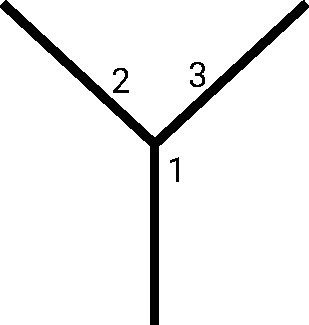
\includegraphics[width=0.15\linewidth]{bc_1.pdf}
\caption{Cхема точки разветвления сосудов}\label{fig:bc_1}
\end{figure}

Рассматриваемые области расчёта включаюи точки,
где сосуды разветвляются. Будем рассматривать только простые разветвления,
когда к одной точке подходит три сосуда (см. схему на рис.~\ref{fig:bc_1}).
Гиперболический характер рассматриваемой системы говорит о том,
что для сопряжения течений в этих трёх сосудах необходимо задать три условия сопряжения.

Первое из этих условий очевидно следует из сохранения расходов:
\begin{equation}
\label{eq:q_conservation}
a_1 u_1 = a_2 u_2 + a_3 u_3.
\end{equation}
Другие два условия связаны с соотношениями для давления. В простейшем случае можно задать равенство
полного давления $\gls{P} = p + u^2/2$:
\begin{equation}
\label{eq:p_total_conservation}
P_1 = P_2 = P_3.
\end{equation}
Это условие моделирует идеальное прохождение разветвления без потерь давления.
Более сложные условия, моделирующие потери давления в зависимости от угла поворота
сосудов при разветвлении, рассматриваются в работе~\cite{Formaggia2003}.

\glsxtrnewsymbol[description={шаг по времени, [с]}]{dt}{\ensuremath{\dt}}
\glsxtrnewsymbol[description={шаг по пространству, [м]}]{dx}{\ensuremath{\dx}}
\glsxtrnewsymbol[description={степень неявности дискретизации по времени}]{theta}{\ensuremath{\theta}}

\section{Методика численного решения}
\subsection{Аппроксимация по пространству. Метод разрывных конечных элементов}
Аппроксимацию системы 
\cref{eq:vector_system}
будем проводить методом разрывных конечных элементов~\cite{dipietro2012}.
Следуя стандартной процедуре этого метода домноженим
исходное уравнение на базисную функцию,
проинтегируем по конечному элементу $E$
применим формулу интегрирования по частям.
Получим
\begin{equation*}
\sum\limits_j M_{ij} \left(\dfr{\vec U}{t}\right)_j 
+ \sum\limits_j T_{ij} \vec F_j + \left.\vec{\bar F} \phi_i \right|_{x_l}^{x_r}
= 
\sum\limits_j M_{ij} \vec B_j.
\end{equation*}
Здесь $M_{ij}$, $T_{ij}$ -- коэффициенты матрица масс и переноса, 
\begin{equation}
\nonumber
M_{ij} = \int\phi_i\phi_j\, dx,
\qquad
T_{ij} = -\int\phi_i\dfr{\phi_j}{x}\, dx.
\end{equation}
Эти матрицы являются блочно-диагональными (или сводятся к блочнодиагональным
в результате перенумерации узлов сетки).
Значение блока этих матрицы при применении линейных и квадратичных
Лагранжевых базисных функций имеют вид:
\begin{align*}
&M^e_{ij} = \frac{\dx}{2}\left(\begin{array}{cc}
2/3 & 1/3\\
1/3 & 2/3\\
\end{array}\right)
\quad
T^e_{ij} = \left(\begin{array}{cc}
0.5 & 0.5 \\ -0.5 & -0.5
\end{array}\right)
\\
&M^e_{ij} = \frac{\dx}{2}\left(\begin{array}{ccc}
	4 / 15 & -1 / 15 &  2 / 15 \\
	-1 / 15 &  4 / 15 &  2 / 15 \\
	2 / 15 &  2 / 15 & 16 / 15
\end{array}\right)
\quad
T^e_{ij} = \left(\begin{array}{ccc}
1 / 2 & -1 / 6 & 2 / 3\\
1 / 6 & -1 / 2 & -2 / 3\\
-2 / 3 & 2 / 3 & 0
\end{array}\right)
\end{align*}
где \gls{dx} -- разбиение области по пространству.
$\phi_i$ -- базисная функция с глобальным индексом $i$,
а $x_l$, $x_r$ -- левая и правая точки элемента, которому принадлежит базисная функция $\phi_i$
(по методике разрывных элементов каждый базис лежит внутри единственнго элемента).
Величина $\vec{\bar F}$ -- противопотоковое значение $\vec F$ в выбранной точке.

\subsection{Аппроксимация по времени}

Дискретизацию по времени с шагом \gls{dt} будем проводить согласно $\theta$ - схеме:
\begin{equation}
\label{eq:time_discretization}
\sum\limits_j M_{ij} \frac{\vec{\hat U_j} - \vec U_j}{\dt}
+ \left( \sum\limits_j T_{ij} \vec F_j + \left.\vec{\bar F} \phi_i \right|_{x_l}^{x_r} \right)^\theta
= 
\left(\sum\limits_j M_{ij} \vec B_j\right)^\theta,
\end{equation}
где символом $\hat \cdot$ обозначено значение на следующем временном слое и введена \gls{theta} -- степень неявности схемы как
\begin{equation*}
\left(Y\right)^\theta = \theta \hat Y + (1 - \theta) Y.
\end{equation*}
При $\theta=0$ мы получаем чисто явную схему, при $\theta = 1$ -- чисто неявную, а выбор $\theta = 1/2$ 
даёт схему Кранка-Николсон второго порядка точности.

В случае $\theta > 0$ выражение \cref{eq:time_discretization} 
является нелинейным относительно неизвестного вектора $\vec U$.
Для его решения требуется линеаризация.

\subsection{Итерационная расчётная схема}
Линеризацию будем проводить за счёт итерационного процесса на временном слое.
Обозначим верхним индексом $\cdot^{n}$ значение на прошлой (известной) итерации,
а $\cdot^{n+1}$ -- значение на текущей (подлежащей определению) итерации.
Тогда окончательно расчётная схема на итерации внутри временного слоя 
на основе дискретизованного соотношения \cref{eq:time_discretization}
примет вид
\begin{align}
&
\label{eq:iter1}
\sum\limits_j M_{ij} \frac{a^{n+1}_j - a_j}{\dt} + \theta\sum\limits_j T_{ij} a_j^{n+1} u_j^{n} = \ldots
\\
&
\nonumber
\qquad\qquad
= -(1 - \theta)\sum\limits_j T_{ij}a_j u_j
- \left(\left(\theta q(\bar a^n, \bar u^n) + (1-\theta)q(\bar a,\bar u)\right)\phi_i\right|_{x_l}^{x_r} \\
\label{eq:iter2}
&
p_j^{n+1} = \frac{\beta}{A}\left(\sqrt{a_j^{n+1}} - \sqrt{A}\right)\\
& 
\label{eq:iter3}
\sum\limits_j M_{ij} \frac{u^{n+1}_j - u_j}{\dt} + 
\theta\sum\limits_j\left(
\frac{T_{ij}u_j^{n}}{2} + \frac{K_\nu M_{ij}}{a_j^{n+1}}
\right)u_j^{n+1} = \dots
\\
&
\nonumber
\qquad\qquad
= -(1 - \theta)
\sum\limits_j\left(
\frac{T_{ij}u_j}{2} + \frac{K_\nu M_{ij}}{a_j}
\right)u_j
\\
&
\nonumber
\qquad\qquad
\phantom{=}
-\theta \sum\limits_j T_{ij} \frac{p^{n+1}_j}{\rho}
-(1 - \theta) \sum\limits_j T_{ij} \frac{p_j}{\rho}
\\
&
\nonumber
\qquad\qquad
\phantom{=}
-\frac1\rho\left(\left(\theta P(\bar a^n, \bar u^n) + (1-\theta)P(\bar a,\bar u)\right)\phi_i\right|_{x_l}^{x_r}
\end{align}

На первом этапе решается уравнение \cref{eq:iter1} и находятся значения $a$ на
текущей итерации. Затем по этому значению определяются значения давления согласно \cref{eq:iter2}
и потом решается уравнение для скорости \cref{eq:iter3}.

Итерации на временном слое продолжаются, пока невязка уравнений
\cref{eq:iter1,eq:iter2} при замене $n+1$ на $n$ не станет меньше
заданного $\epsilon=10^{-8}$.

\subsubsection{Вычисление противопотоковых значений фуункций}
Вычисление значений $\bar a$, $\bar u$, которые используются для вычисления
численных потоков в уравнениях \cref{eq:iter1,eq:iter3} будем проводить на основе подхода~\cite{Sherwin2003}.

Как было отмечено ранее, естественные переменные содержат в себе разнонаправленные возмущения, поэтому
не могут быть использованы напрямую для вычисления противопотоковых значений $\bar u, \bar a$.
Поэтому используем переменные Римана. 
Будем рассматривать соединения двух типов: двух и трёх элементов. Их локальная нумерация
представлена на рис.~\ref{fig:bc_2}.

\begin{figure}[h]
    \centering
    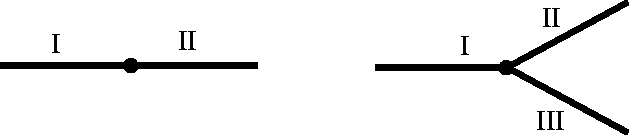
\includegraphics[width=0.6\linewidth]{bc_2.pdf}
    \caption{Локальная нумерация эелементов при рассмотрении сочленения}
    \label{fig:bc_2}
\end{figure}

C учётом выбранного направления движения $w_1$ слева направо
вычислим противопотоковые значения переменных Римана как
\begin{equation*}
\bar w_1 = u_I + 4 (c_I - c_0), \quad \bar w_2 = u_{II} - 4 (c_{II} - c_0), \quad \bar w_3 = u_{III} - 4 (c_{III} - c_0).
\end{equation*}
Значения $u,c_{I,II,III}$ - есть значение функций в точке сочленения, взятое
со стороны соответствующего элемента. Эти значения берутся с известного итерационного слоя.

При рассмотрения линейного сочленения (правый из рисунков \ref{fig:bc_2})
далее пользуясь определением \cref{eq:w12_def}
запишем уравнения
\begin{equation}
\label{eq:sys2}
\begin{aligned}
&\bar w_1 = \bar u_1 + 4 (\bar c_1 - c_0), \\
&\bar w_2 = \bar u_2 - 4 (\bar c_2 - c_0)
\end{aligned}
\end{equation}
В случае, если физические свойства ($\beta$ и $A$) не терпят разрыв в точке сочленения,
то $\bar u_1 = \bar u_2$, $\bar c_1 = \bar c_2$ и эта система
может быть разрешена с помощью выражений
\cref{eq:ua_from_w}. Иначе её следует дополнить двумя уравнениями сохранения: расхода и полного давления
\begin{equation}
\label{eq:sys1}
\begin{aligned}
&q(\bar u_1, \bar a_1) = q(\bar u_2, \bar a_2), \\
&P(\bar u_1, \bar a_1) = P(\bar u_2, \bar a_2)
\end{aligned}
\end{equation}
Нелинейная система \cref{eq:sys1,eq:sys2} может быть решена итерационным решателем (например, методом Ньютона).

В случае разветвления сосудов (правая схема на рис.~\ref{fig:bc_2}), аналогичная система уравнений,
дополненная условиями разрешимости на основе \cref{eq:q_conservation,eq:p_total_conservation} примет вид

\begin{equation}
\label{eq:sys3}
\begin{aligned}
&\bar w_1 = \bar u_1 + 4 (\bar c_1 - c_0), \\
&\bar w_2 = \bar u_2 - 4 (\bar c_2 - c_0), \\
&\bar w_3 = \bar u_3 - 4 (\bar c_3 - c_0), \\
&q(\bar u_1, \bar a_1) = q(\bar u_2, \bar a_2) + q(\bar u_3, \bar a_3), \\
&P(\bar u_1, \bar a_1) = P(\bar u_2, \bar a_2), \\
&P(\bar u_1, \bar a_1) = P(\bar u_3, \bar a_3).
\end{aligned}
\end{equation}

\section{Верификация и результаты расчётов}

\glsxtrnewsymbol[description={частота сердцебиения, [ударов/мин]}]{bpm}{\ensuremath{bpm}}
\glsxtrnewsymbol[description={$=c_0\dt/\dx$, число Куранта, рассчитанное по скорости $c_0$, [1]}]{CFL}{\ensuremath{\CFL}}

\subsection{Течение в однородном одиночном сосуде}
Верификацию численного метода начнём с
простейшей задачи о переносе
единственного импульса (волны давления) в
одиночном сосуде.
Задача решалась в двух постановках, заимствованных из работы~\cite{boileau:2015}. В первом вариант рассматривалась невязкая жидкость,
во втором использовалось значение $\mu = 4$мПа$\cdot$с.
Физические параметры задачи представлены в таблице ниже

\begin{equation}
\nonumber
\begin{array}{l|c|c}
\text{параметр}  & \text{вариант 1} & \text{вариант 2}\\
\hline
\text{длина, м} & \multicolumn{2}{c}{10.0}\\
\hline
R\text{, см} & \multicolumn{2}{c}{1.0}\\
\hline
E\text{, МПа} & \multicolumn{2}{c}{0.4}\\
\hline
h\text{, мм} & \multicolumn{2}{c}{1.5}\\
\hline
\rho\text{, кг/м\textsuperscript{3}} & \multicolumn{2}{c}{1050}\\
\hline
\mu\text{, мПа$\cdot$с} & 0 & 4\\
\hline
\zeta & \multicolumn{2}{c}{9}\\
\hline
\end{array}
\end{equation}

В качестве входных граничных условий задавалось
значение расхода, соответствующее экспоненциальному пику на значении $q=10^{-6}$ м$^3$/c в момент $t=0.05$ с:
\begin{equation*}
q_{in}(t) = 10^{-6}\exp(-10^4(t-0.05)^2).
\end{equation*}
Таким образом, максимальная скорость течения жидкости
составляла около $3$ мм/с.
При этом скорость распространения возмущений
составляла $c_0\approx6.17$ м/c.

Известно~\cite{boileau:2015}, что решением рассматриваемой задачи
в варианте 1 является единственная волна давления с постоянной высотой $p_{max}$.
В варианте 2 эта волна давления будем уменьшаться с продвижением по сосуду из-за вязкой диффузии. При
этом пиковое значение этой волны будет равно
\begin{equation}
\label{eq:p_peak_visc}
p_{max, visc}(x) = p_{max} \exp\left(-\frac{(\zeta + 2)\pi \mu x}{\rho c_0 A}\right).
\end{equation}

Для представленных выше постановок
была произведена серия расчётов с различными шагами по времени и пространству
с использованием различных схем дискретизации по времени (разных значений $\theta$)
и по пространству (разных степеней использованных конечных элементов).

Добиться устойчивого решения с использованием элементов высоких порядков точности
не удалось. Таким образом, все дальнейшие вычисления
будут проводиться на линейных Лагранжевых элементах.

Результаты расчёты с использованием разных $\theta$ 
схем в сравнении с результатами~\cite{boileau:2015}
представлены на рис.~\ref{fig:prob2}.
Для этих расчётов использовался шаг по пространству $\dx = 0.01$
и шаг по времени $\dt = 2\cdot10^{-4}$ с,
который обеспечивал устойчивый счёт для схем $\theta=0.5, 1.0$.
Число Куранта, рассчитанное по скорости $c_0$ было равно $\CFL = 0.12$.
Для явной схемы
не удалось подобрать такой шаг по времени, при котором решение
бы не расходилось.  На рис.~\ref{fig:prob2_d}) приведены результаты для $\dt=5\cdot10^{-5}$.
Неявная схема (рис.~\ref{fig:prob2_c}), хоть и демонстрировала условно устойчивое поведение,
но оказалась подвержена большой численной диффузии.
Результаты расчётов по схеме Кранка-Николсон (рис.~\ref{fig:prob2_b})
показали хорошее согласование как с точным решением, так и с численным решением из~\cite{boileau:2015},
представленным на рис.~\ref{fig:prob2_a}.

По результатам рассмотрения этого тестового случая были выработаны следующие
рекомендованные параметры расчётной схемы:
\begin{itemize}
\item Дискретизация по пространству линейными Лагранжевыми конечными элементами;
\item Схема дискретизации по времени с $\theta=0.5$ (Кранка-Николсон);
\item Выбор шага по времени исходя из числа Куранта, рассчитанного по скорости $c_0$, $\gls{CFL} \approx 0.1$.
\end{itemize}
Эти параметры будут использоваться для всех дальнейших расчётов.

\begin{figure}[h!]
\begin{subfigure}{0.5\linewidth}\centering
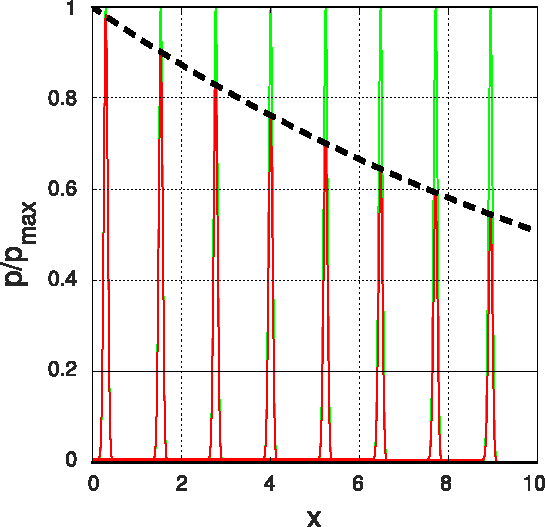
\includegraphics[width=0.9\linewidth]{problem2_article.pdf}
\caption{Результаты из~\cite{boileau:2015}}\label{fig:prob2_a}
\end{subfigure}%
\begin{subfigure}{0.5\linewidth}\centering
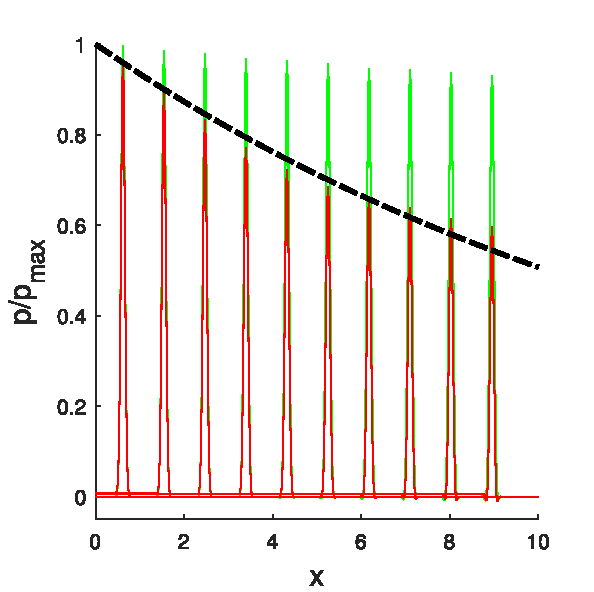
\includegraphics[width=0.9\linewidth]{problem2_theta05.pdf}
\caption{$\theta=0.5$}\label{fig:prob2_b}
\end{subfigure} \\
\hfill \\
\begin{subfigure}{0.5\linewidth}\centering
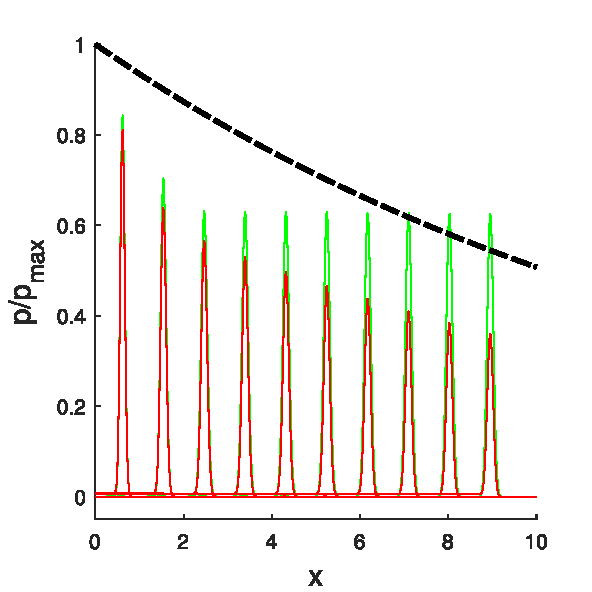
\includegraphics[width=0.9\linewidth]{problem2_theta1.pdf}
\caption{$\theta=1$}\label{fig:prob2_c}
\end{subfigure}%
\begin{subfigure}{0.5\linewidth}\centering
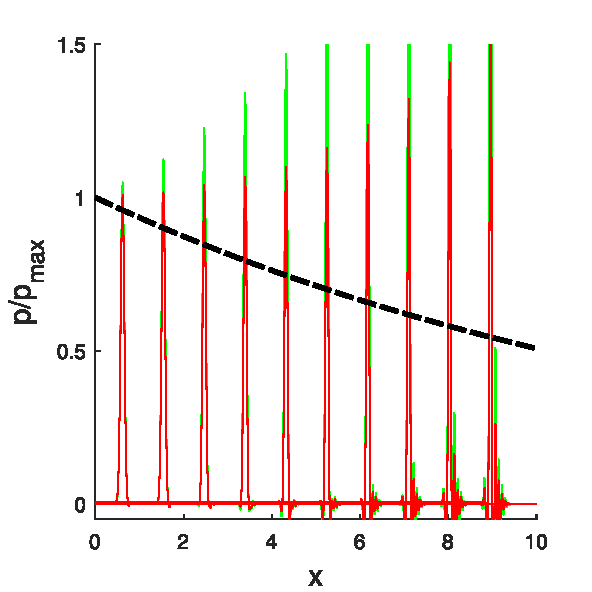
\includegraphics[width=0.9\linewidth]{problem2_theta0.pdf}
\caption{$\theta=0$}\label{fig:prob2_d}
\end{subfigure}%
\caption{Положение скачка давления в различные моменты времени: зелёная линия -- расчёт без вязкости, красная линия -- расчёт с $\mu$=4мПа,
чёрный пунктир -- падение пика давления с продвижением фронта \cref{eq:p_peak_visc}}\label{fig:prob2}
\end{figure}


\subsection{Течение в одиночном сосуде с разрывными свойствами}
\subsubsection{Сосуд со вставкой}

\begin{figure}[h!]
\begin{subfigure}{0.5\linewidth}\centering
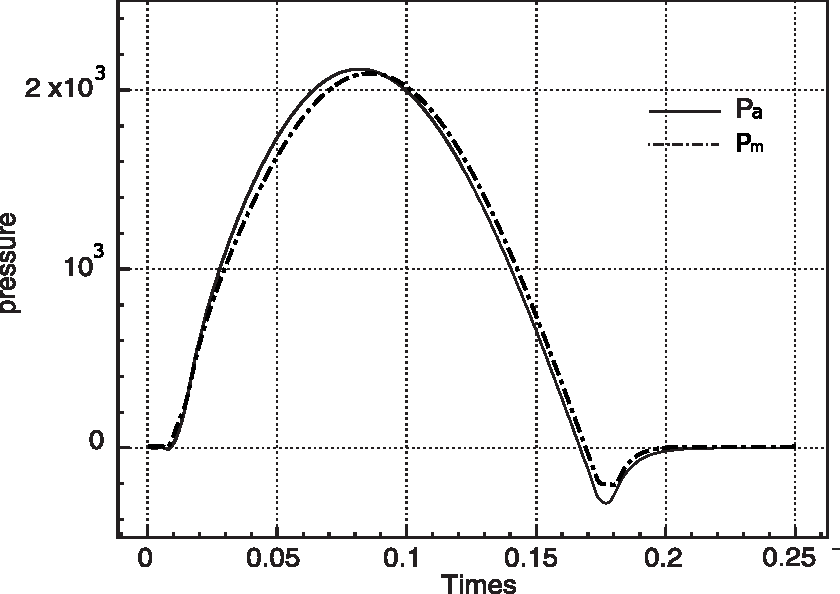
\includegraphics[width=0.9\linewidth]{problem3_P.pdf}
\caption{Контрольная $P$ точка перед вставкой}\label{fig:prob3_a}
\end{subfigure}%
\begin{subfigure}{0.5\linewidth}\centering
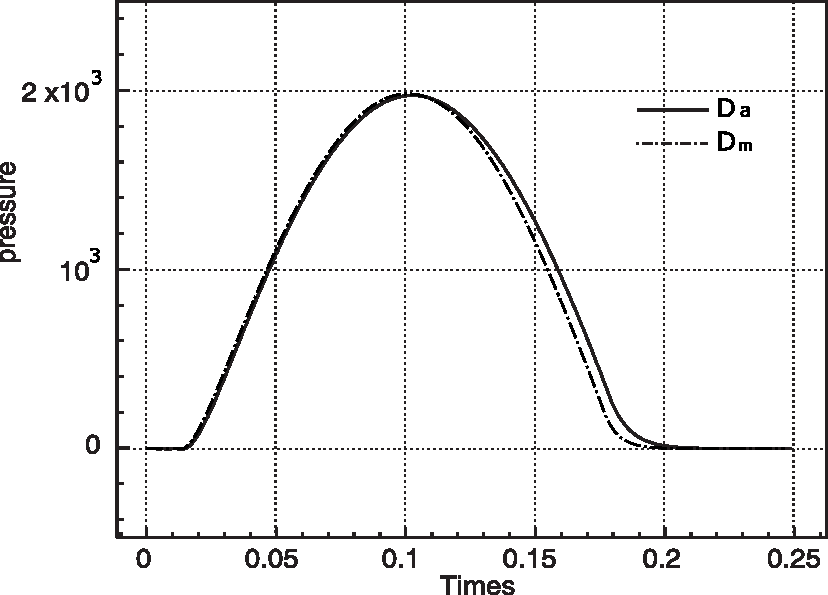
\includegraphics[width=0.9\linewidth]{problem3_D.pdf}
\caption{Контрольная точка $D$ в вставке}\label{fig:prob3_b}
\end{subfigure} \\
\hfill \\
\begin{subfigure}{0.5\linewidth}\centering
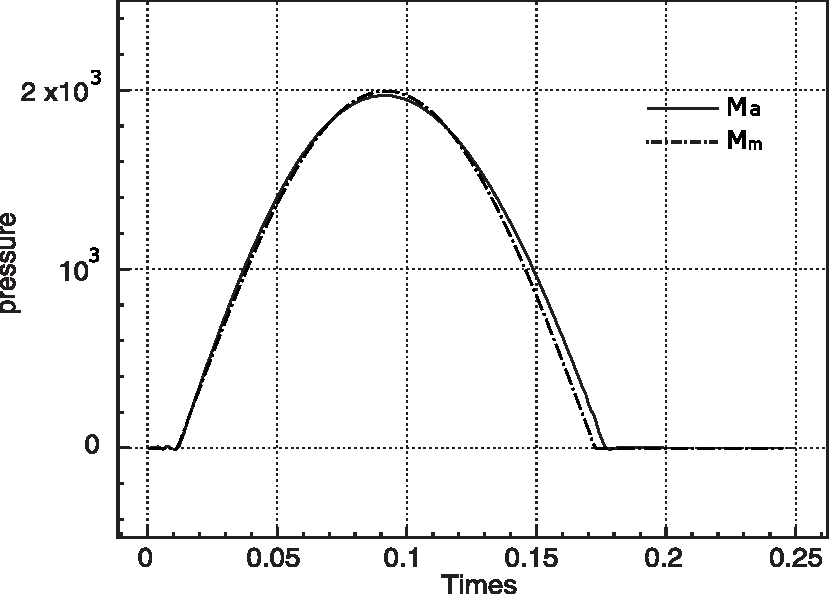
\includegraphics[width=0.9\linewidth]{problem3_M.pdf}
\caption{Контрольная точка $M$ после вставки}\label{fig:prob3_c}
\end{subfigure}%
\caption{Сравнение значения давления в контрольных точках. Сплошная линия -- наш расчёт, пунктирная -- результаты~\cite{Sherwin2003}}\label{fig:prob3}
\end{figure}

\subsubsection{Влияние смены свойств стенок сосуда на решение задачи}
TODO

\subsection{Течение в сосуде с разветвлением}
Рассматривается тестовая задача~\cite{Xiu:2007} о течении в разветвлении сосудов.
Расчётные свойства сосудов до разветвления (сосуд 1) и после разветвления (сосуды 2)
представлены ниже

\begin{equation}
\nonumber
\begin{array}{l|c|c}
\text{параметр}  & \text{сосуд 1} & \text{сосуды 2}\\
\hline
\text{длина, м} & 0.2 & 0.2\\
\hline
R\text{, мм} & 5.0 & 5.0/\sqrt{6}\\
\hline
E\text{, kПа} & 108 & 264.5\\
\hline
h\text{, мм} & \multicolumn{2}{c}{0.1}\\
\hline
\rho\text{, кг/м\textsuperscript{3}} & \multicolumn{2}{c}{1000}\\
\hline
\mu\text{, Па с} & \multicolumn{2}{c}{0}\\
\hline
\end{array}
\end{equation}

В качестве граничного условия использовалось фиксированное входное значение
площади поперечного сечения $a = A$ и зависимость скорости от времени вида:
\begin{equation}
\nonumber
u_{in}(t) = 0.01\exp\left(-5000(t-0.05)^2\right).
\end{equation}
Таким образом, на вход подаётся единичная волна с пиковым
значением скорости $0.01$ м/с в момент времени $0.05$ с.

Расчёты проедены на сетке из 120 конечных элементов
(что соответствовало шагу по пространству $\dx = 0.005$ м)
с шагом по времени $\dt = 2.5\cdot10^{-4}$ с.
При выбранных параметрах сосудов скорость возмущений 
составляла $c_0=1.2$ м/с и $c_0 = 2.94$ м/с
для первого и вторых сосудов соответственно.
То есть число Куранта составляло $\CFL\approx0.15$.


Продвижение волны давления и скорости представлены на рис.~\ref{fig:prob4_pv}.
Поступательная волна повышенного давления и скорости
формируется от входного сечения (рис.~\ref{fig:prob4_pv_a})
и движется вперёд до точки разветвления (рис.~\ref{fig:prob4_pv_b}).
В этой точке происходит отражение части волны назад, после чего
наблюдаются уже две волны (рис.~\ref{fig:prob4_pv_c}):
поступательная волна продолжает движение по выходным сегментам графа,
а возвратная волна повышенного давления и пониженной (отрицательной)
скорости движется к входному сечению.

\begin{figure}[h!]
\begin{subfigure}{1.0\linewidth}\centering
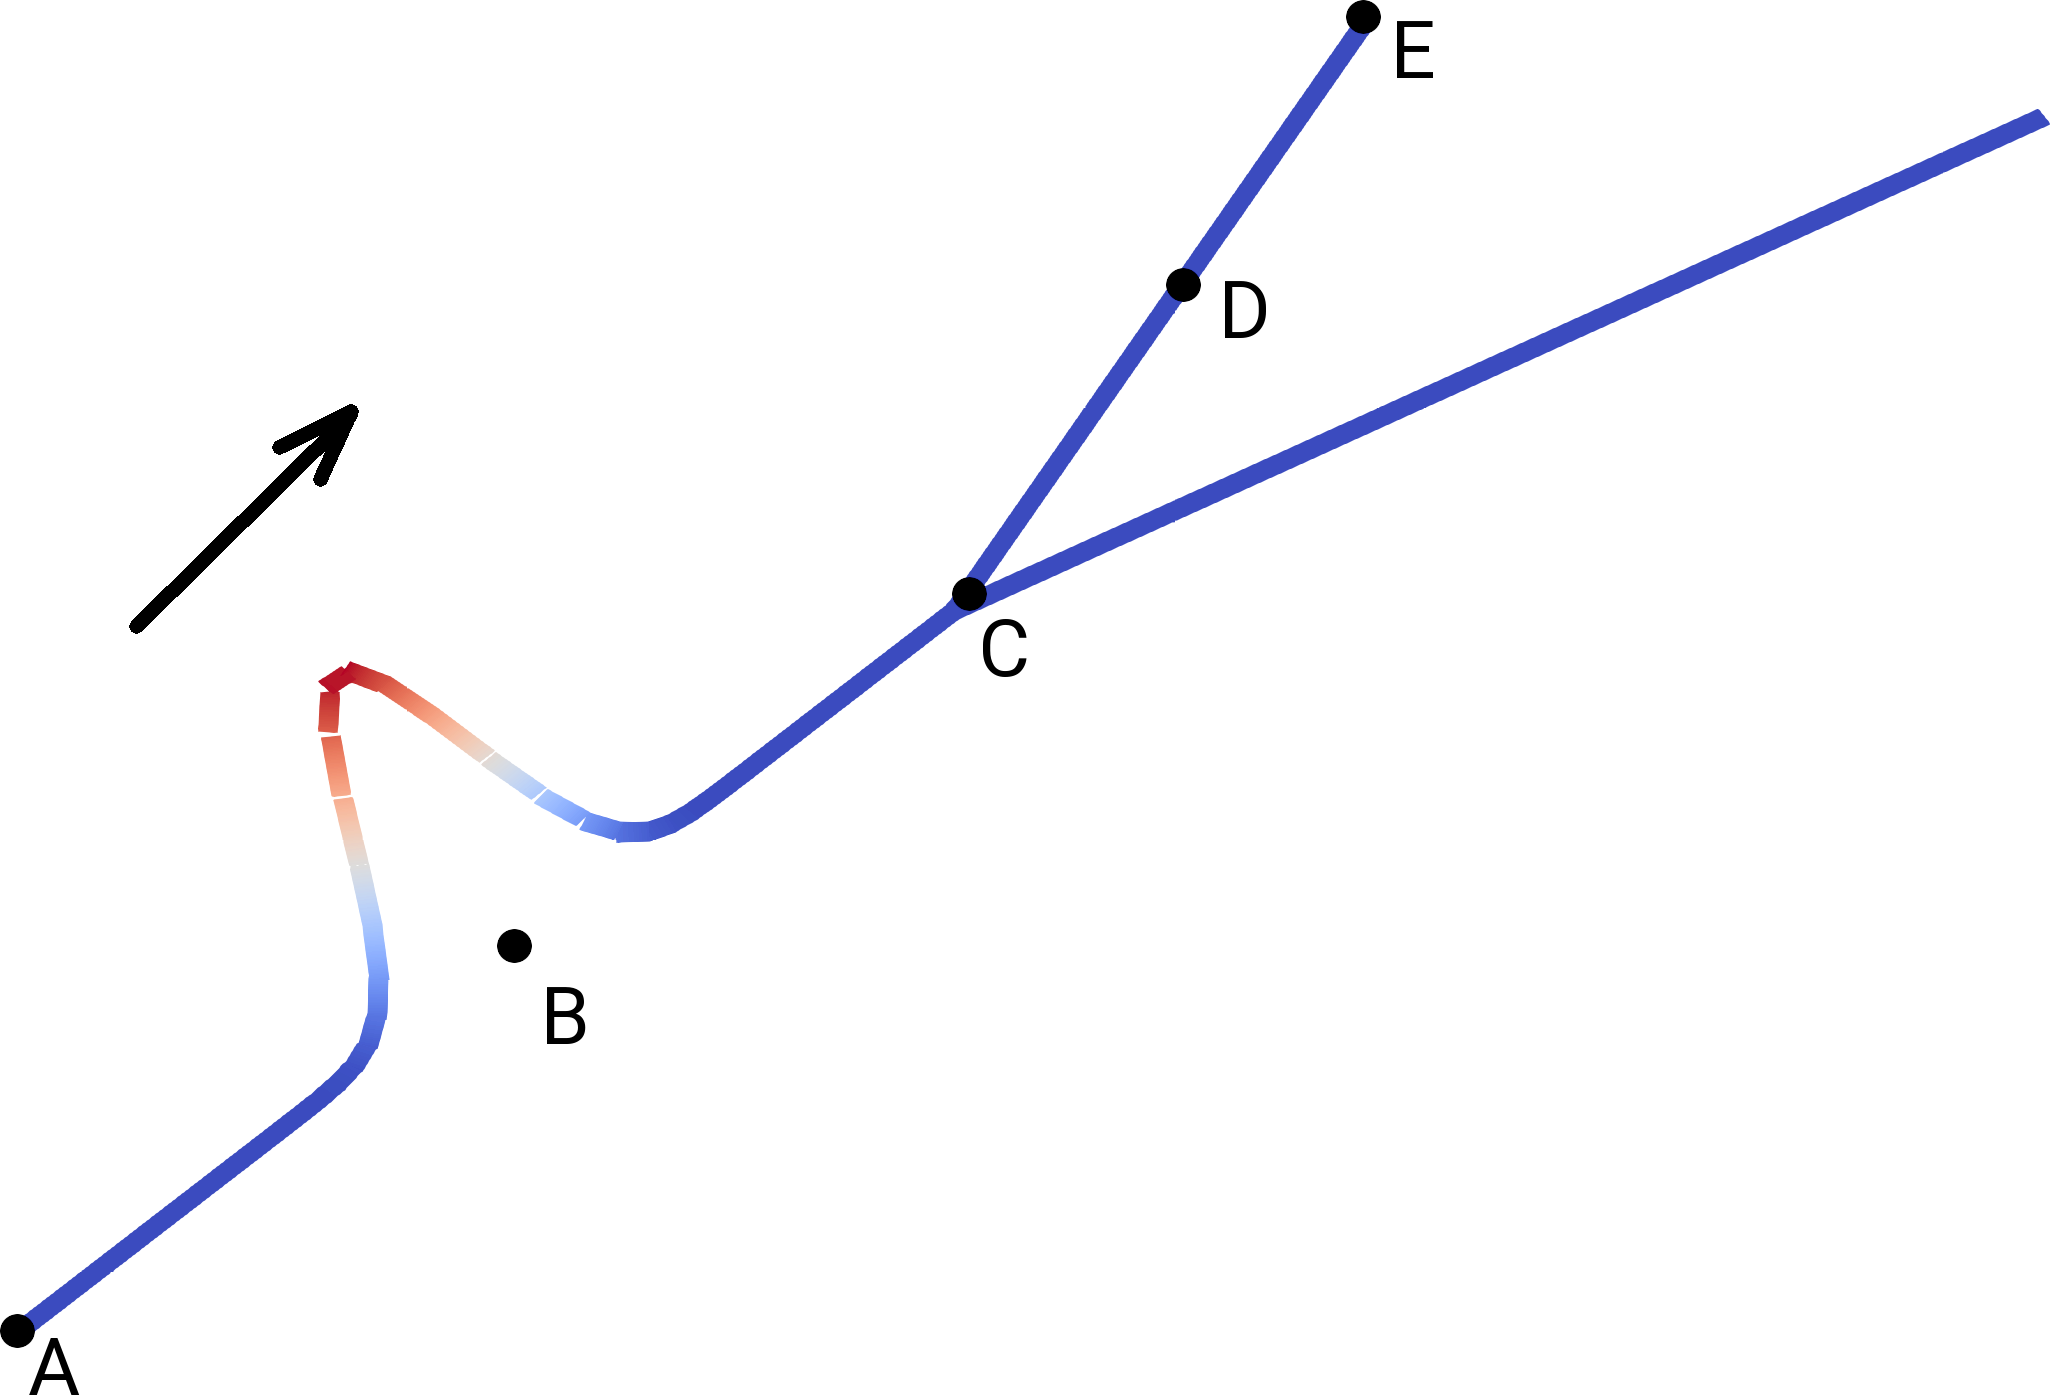
\includegraphics[width=0.4\linewidth]{prob4_time/p0.png}
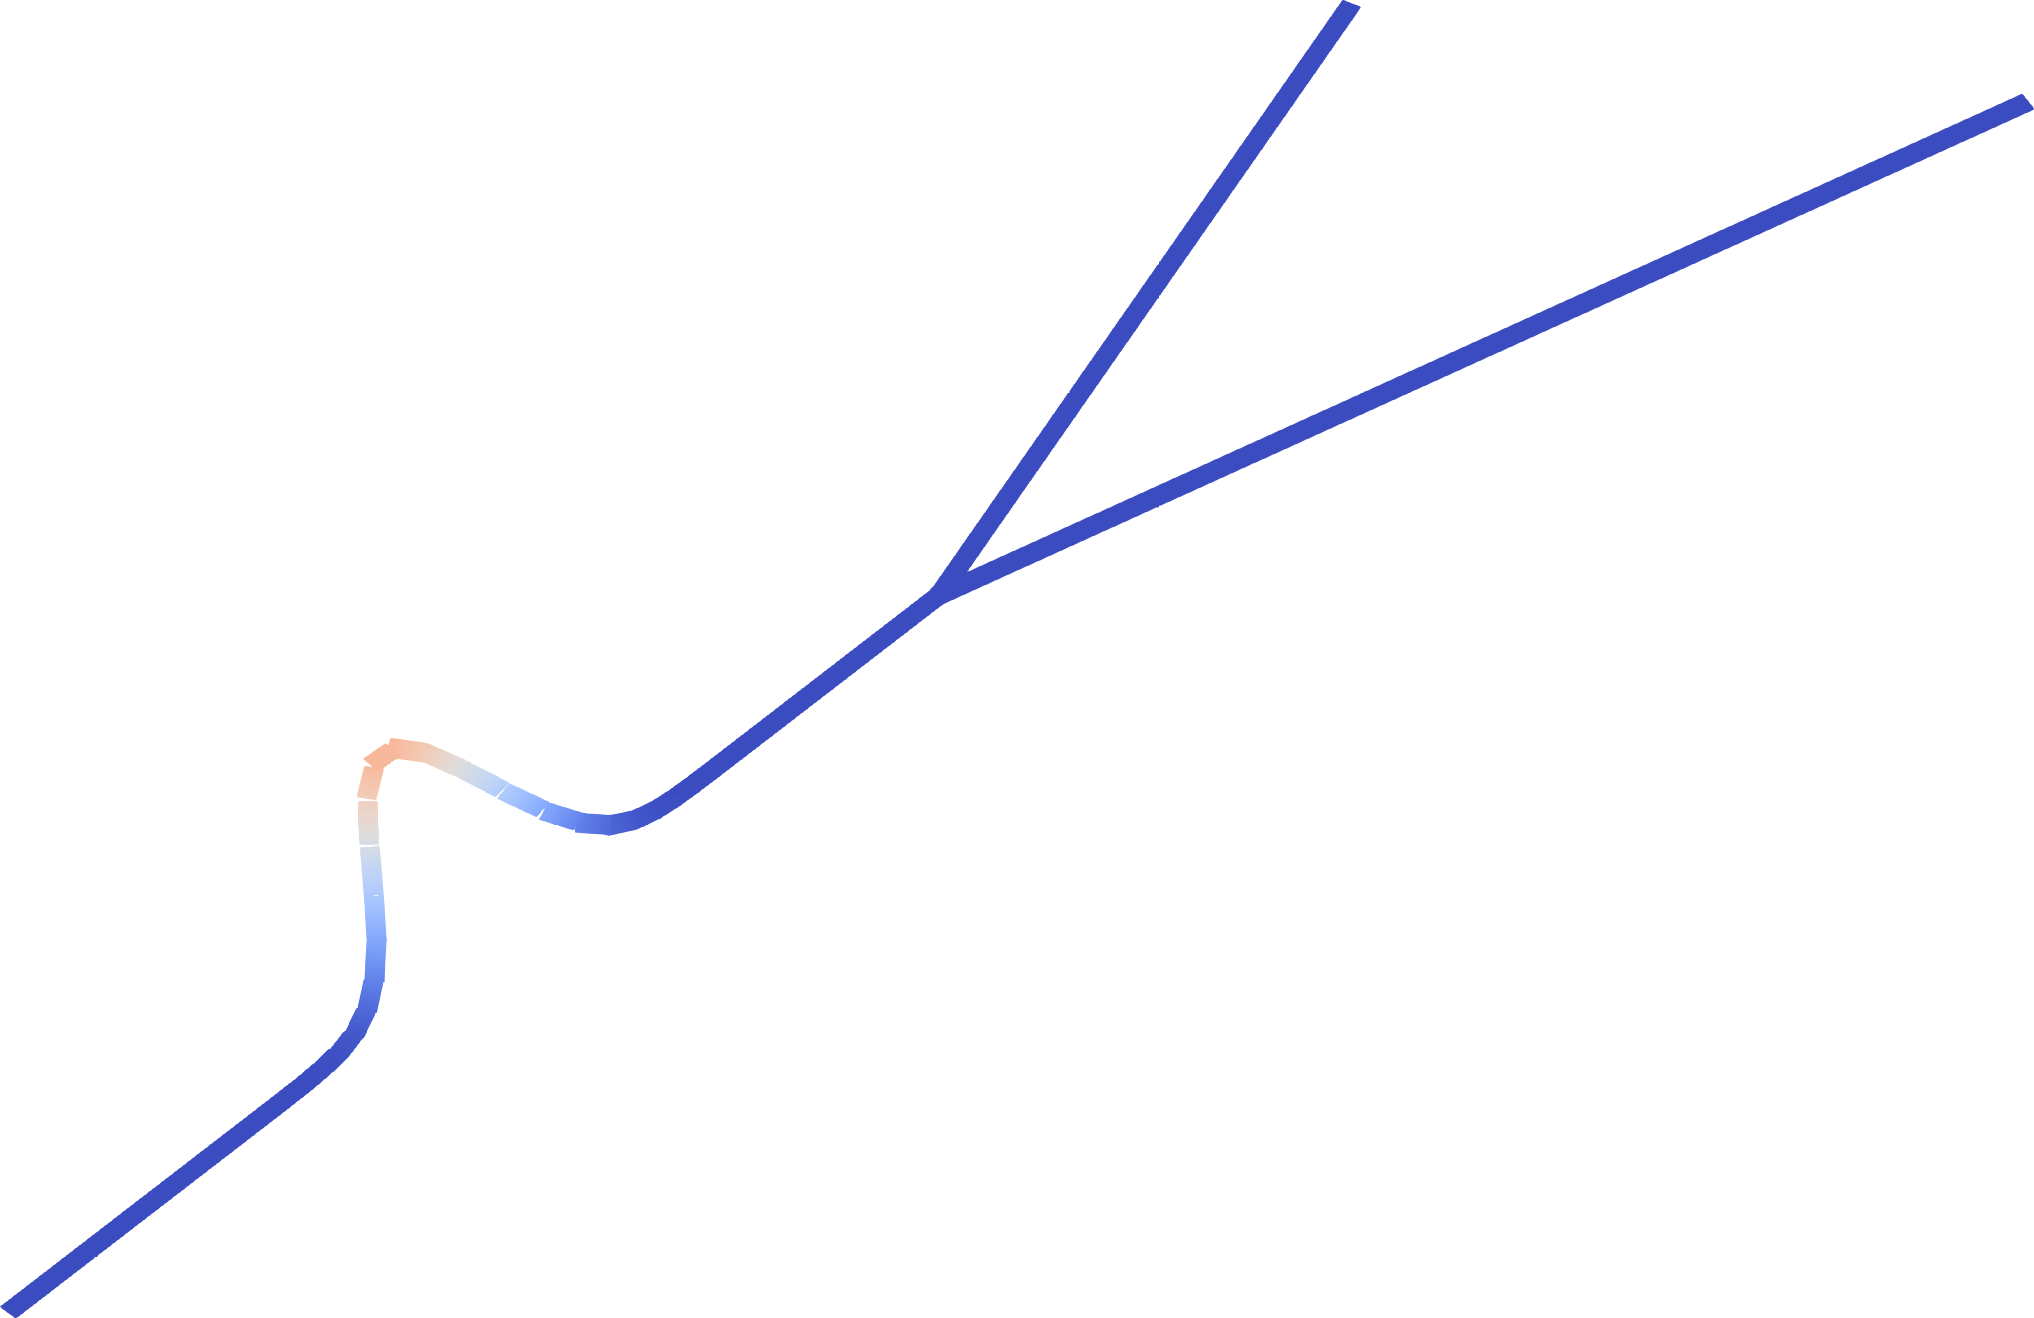
\includegraphics[width=0.4\linewidth]{prob4_time/v0.png}
\caption{$t = 0.13$}\label{fig:prob4_pv_a}
\end{subfigure} \\
\hfill \\
\hfill \\
\begin{subfigure}{1.0\linewidth}\centering
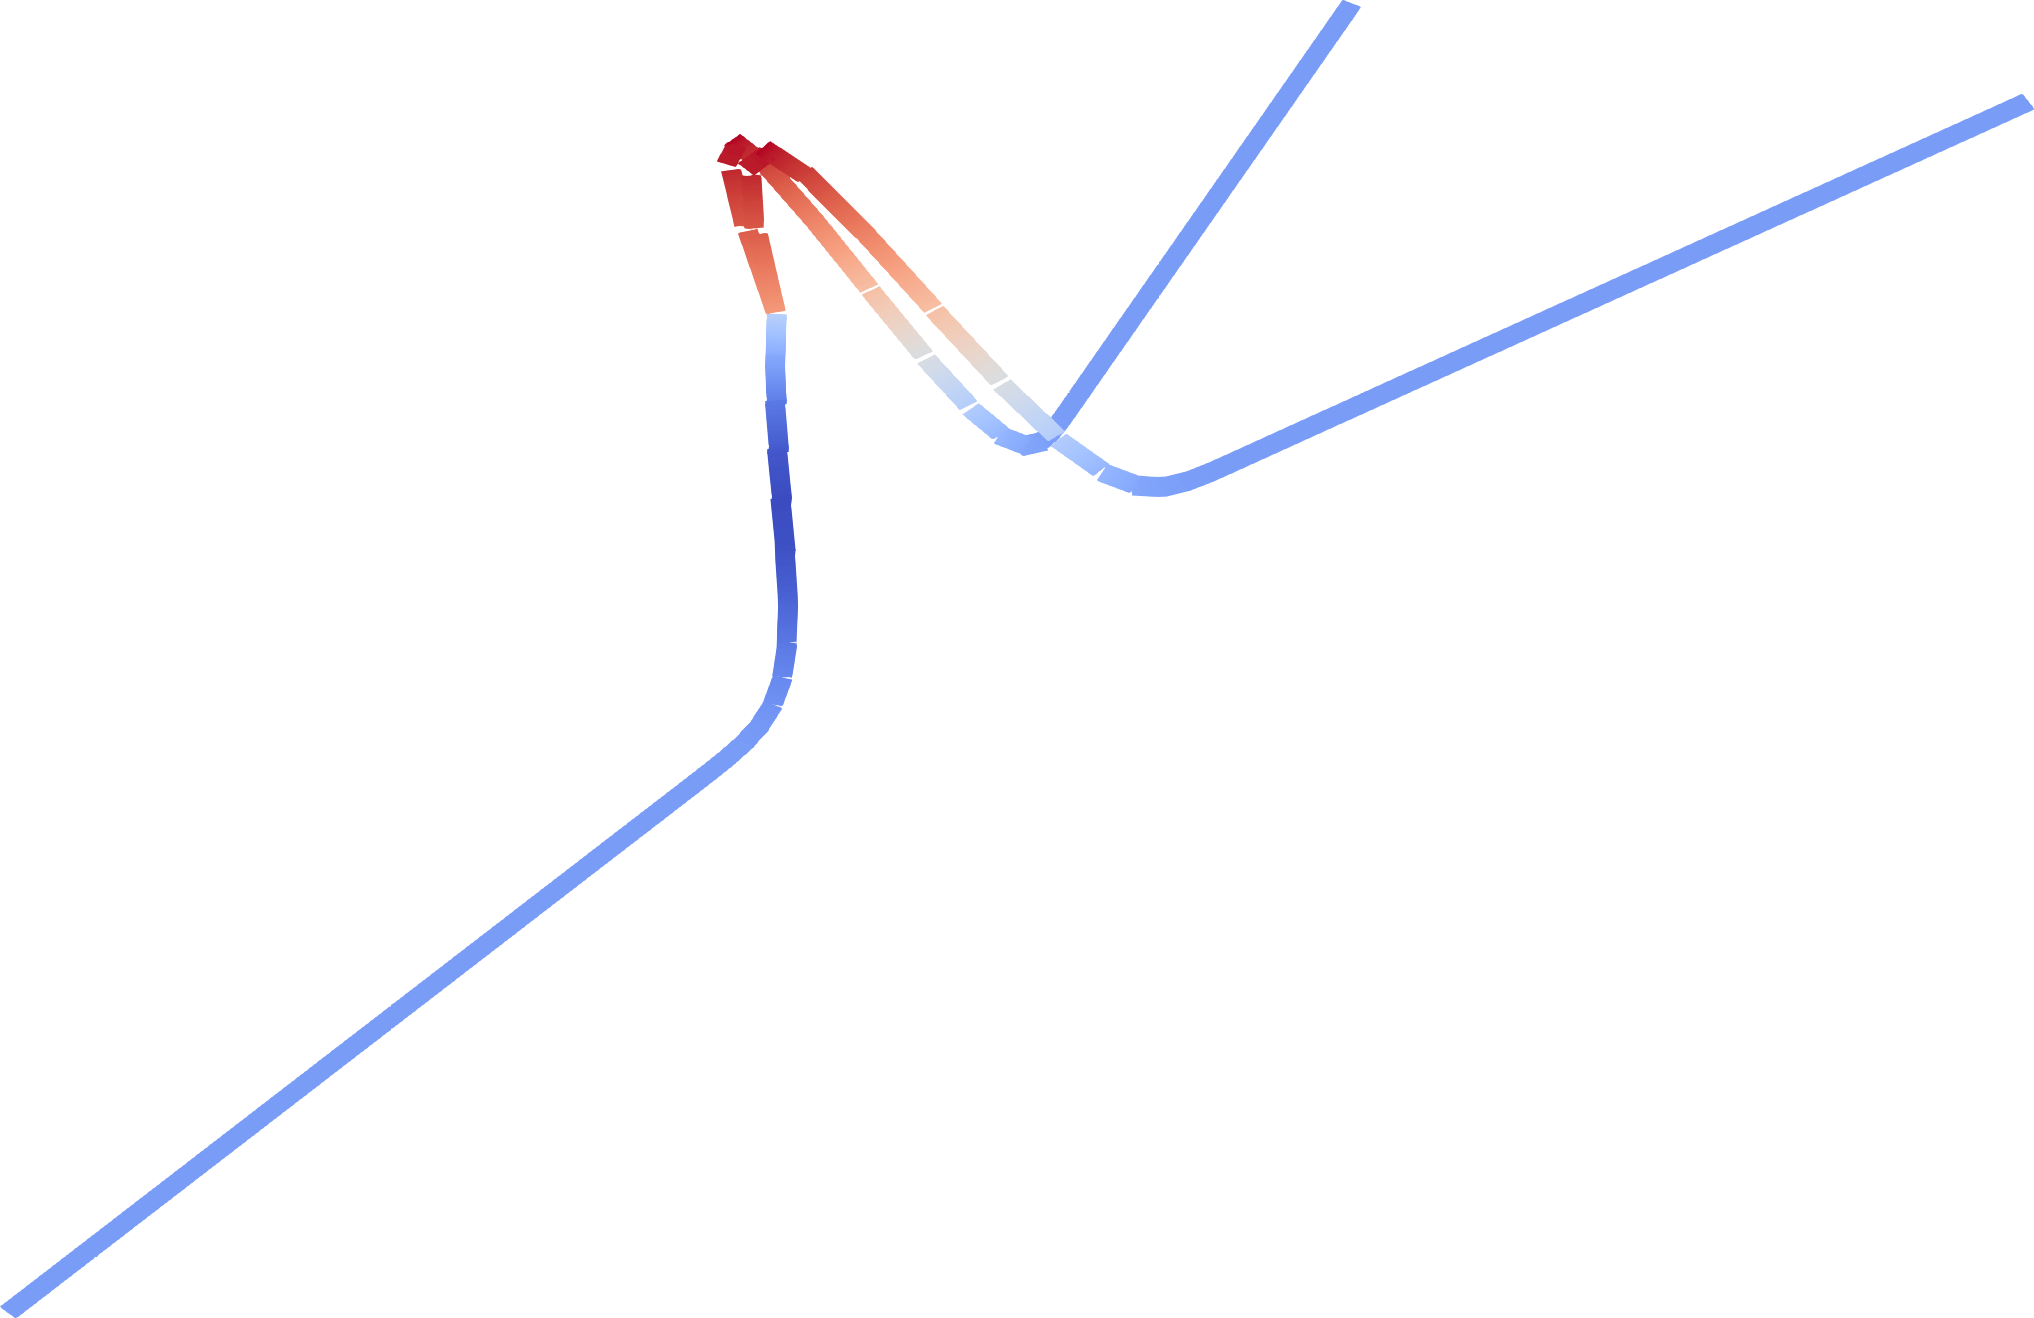
\includegraphics[width=0.4\linewidth]{prob4_time/p1.png}
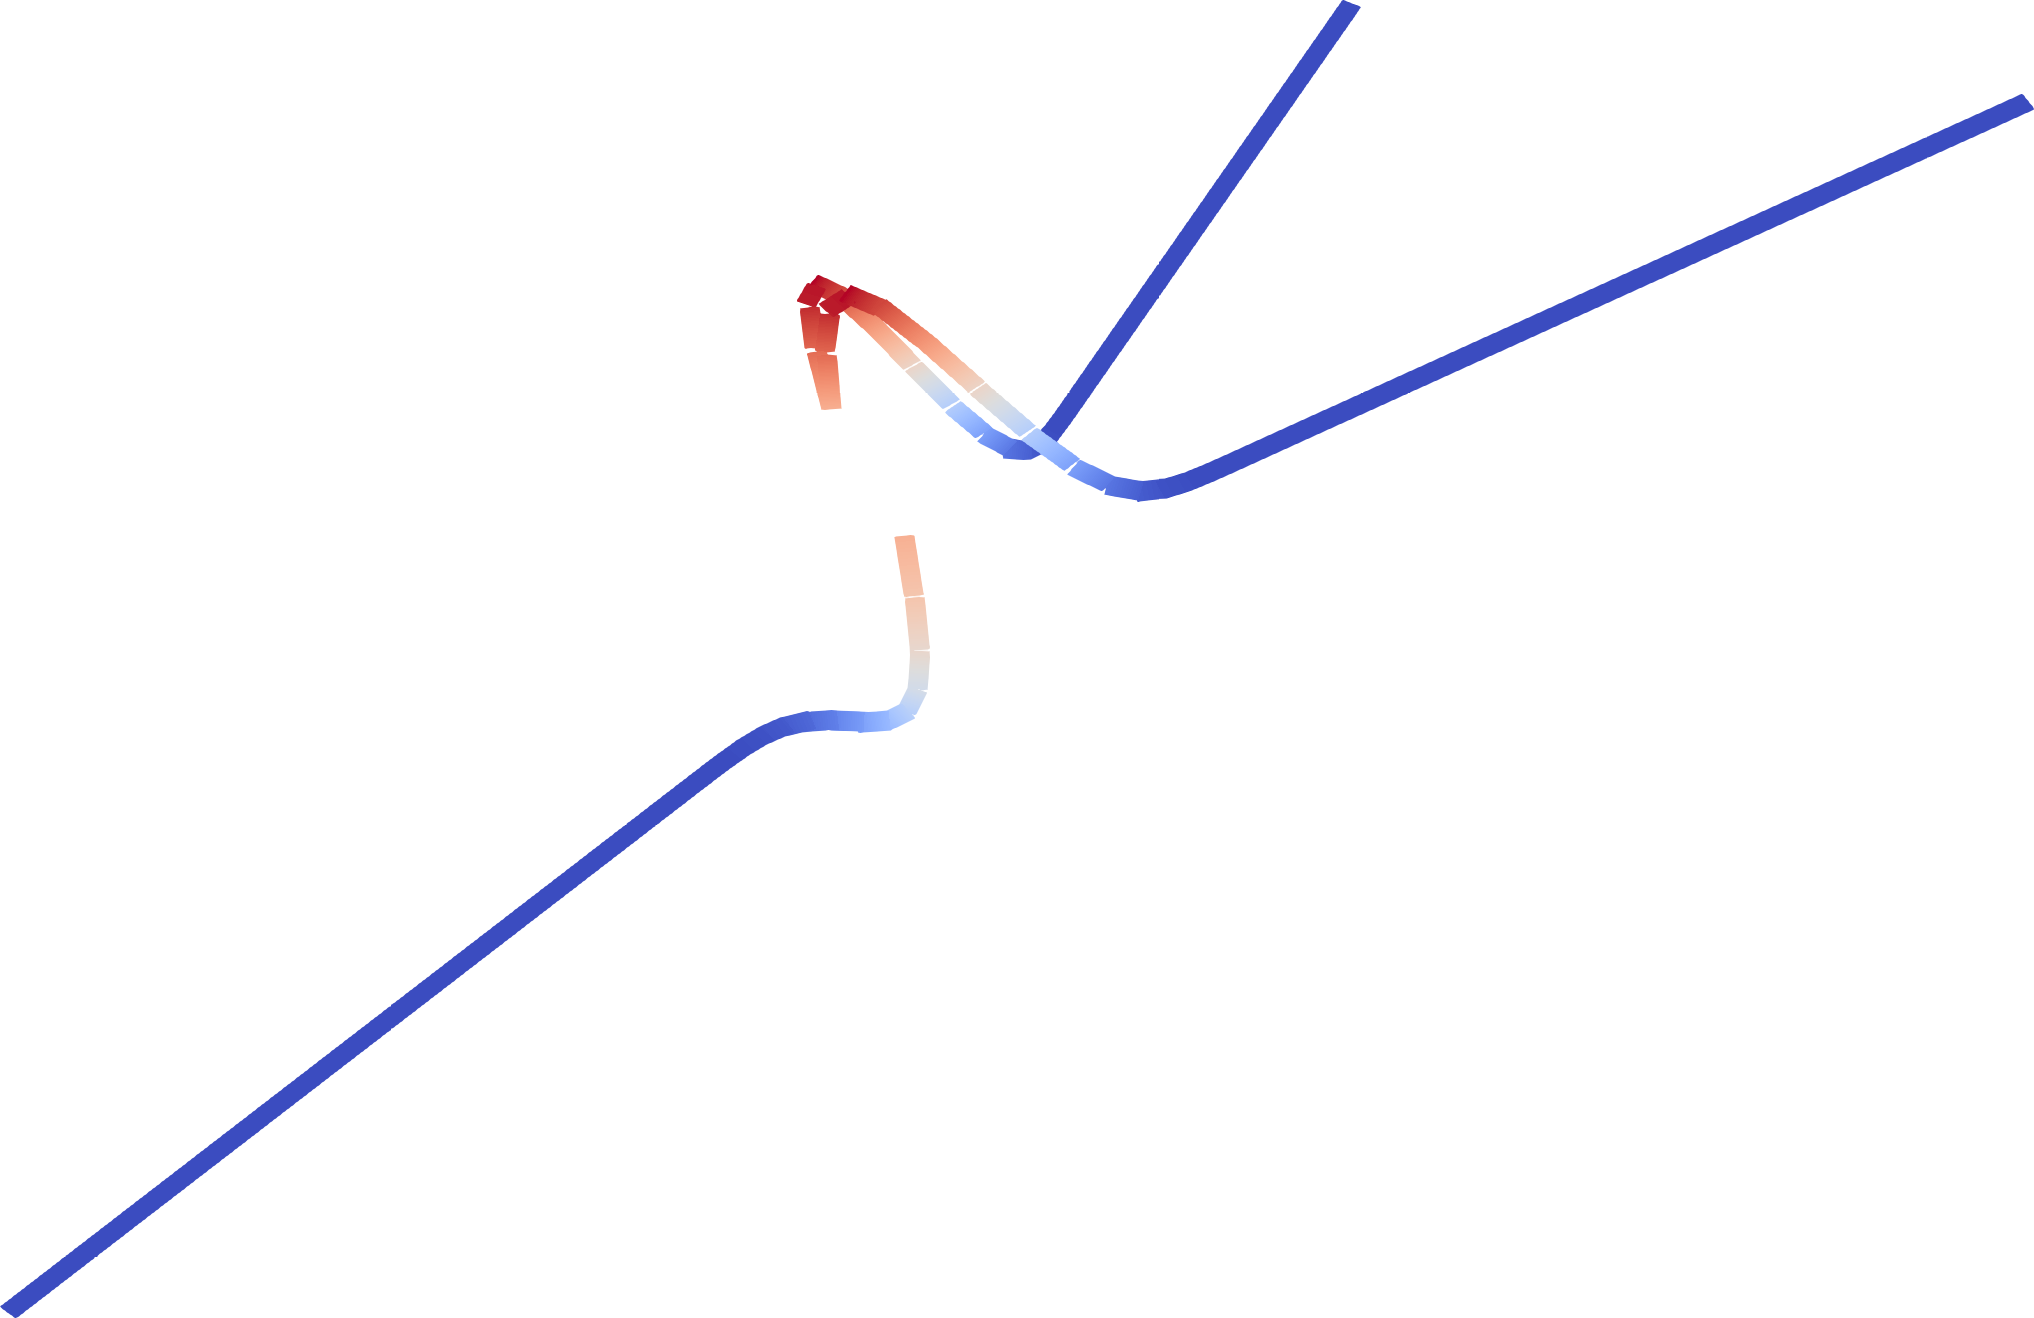
\includegraphics[width=0.4\linewidth]{prob4_time/v1.png}
\caption{$t = 0.22$}\label{fig:prob4_pv_b}
\end{subfigure}\\
\hfill \\
\hfill \\
\begin{subfigure}{1.0\linewidth}\centering
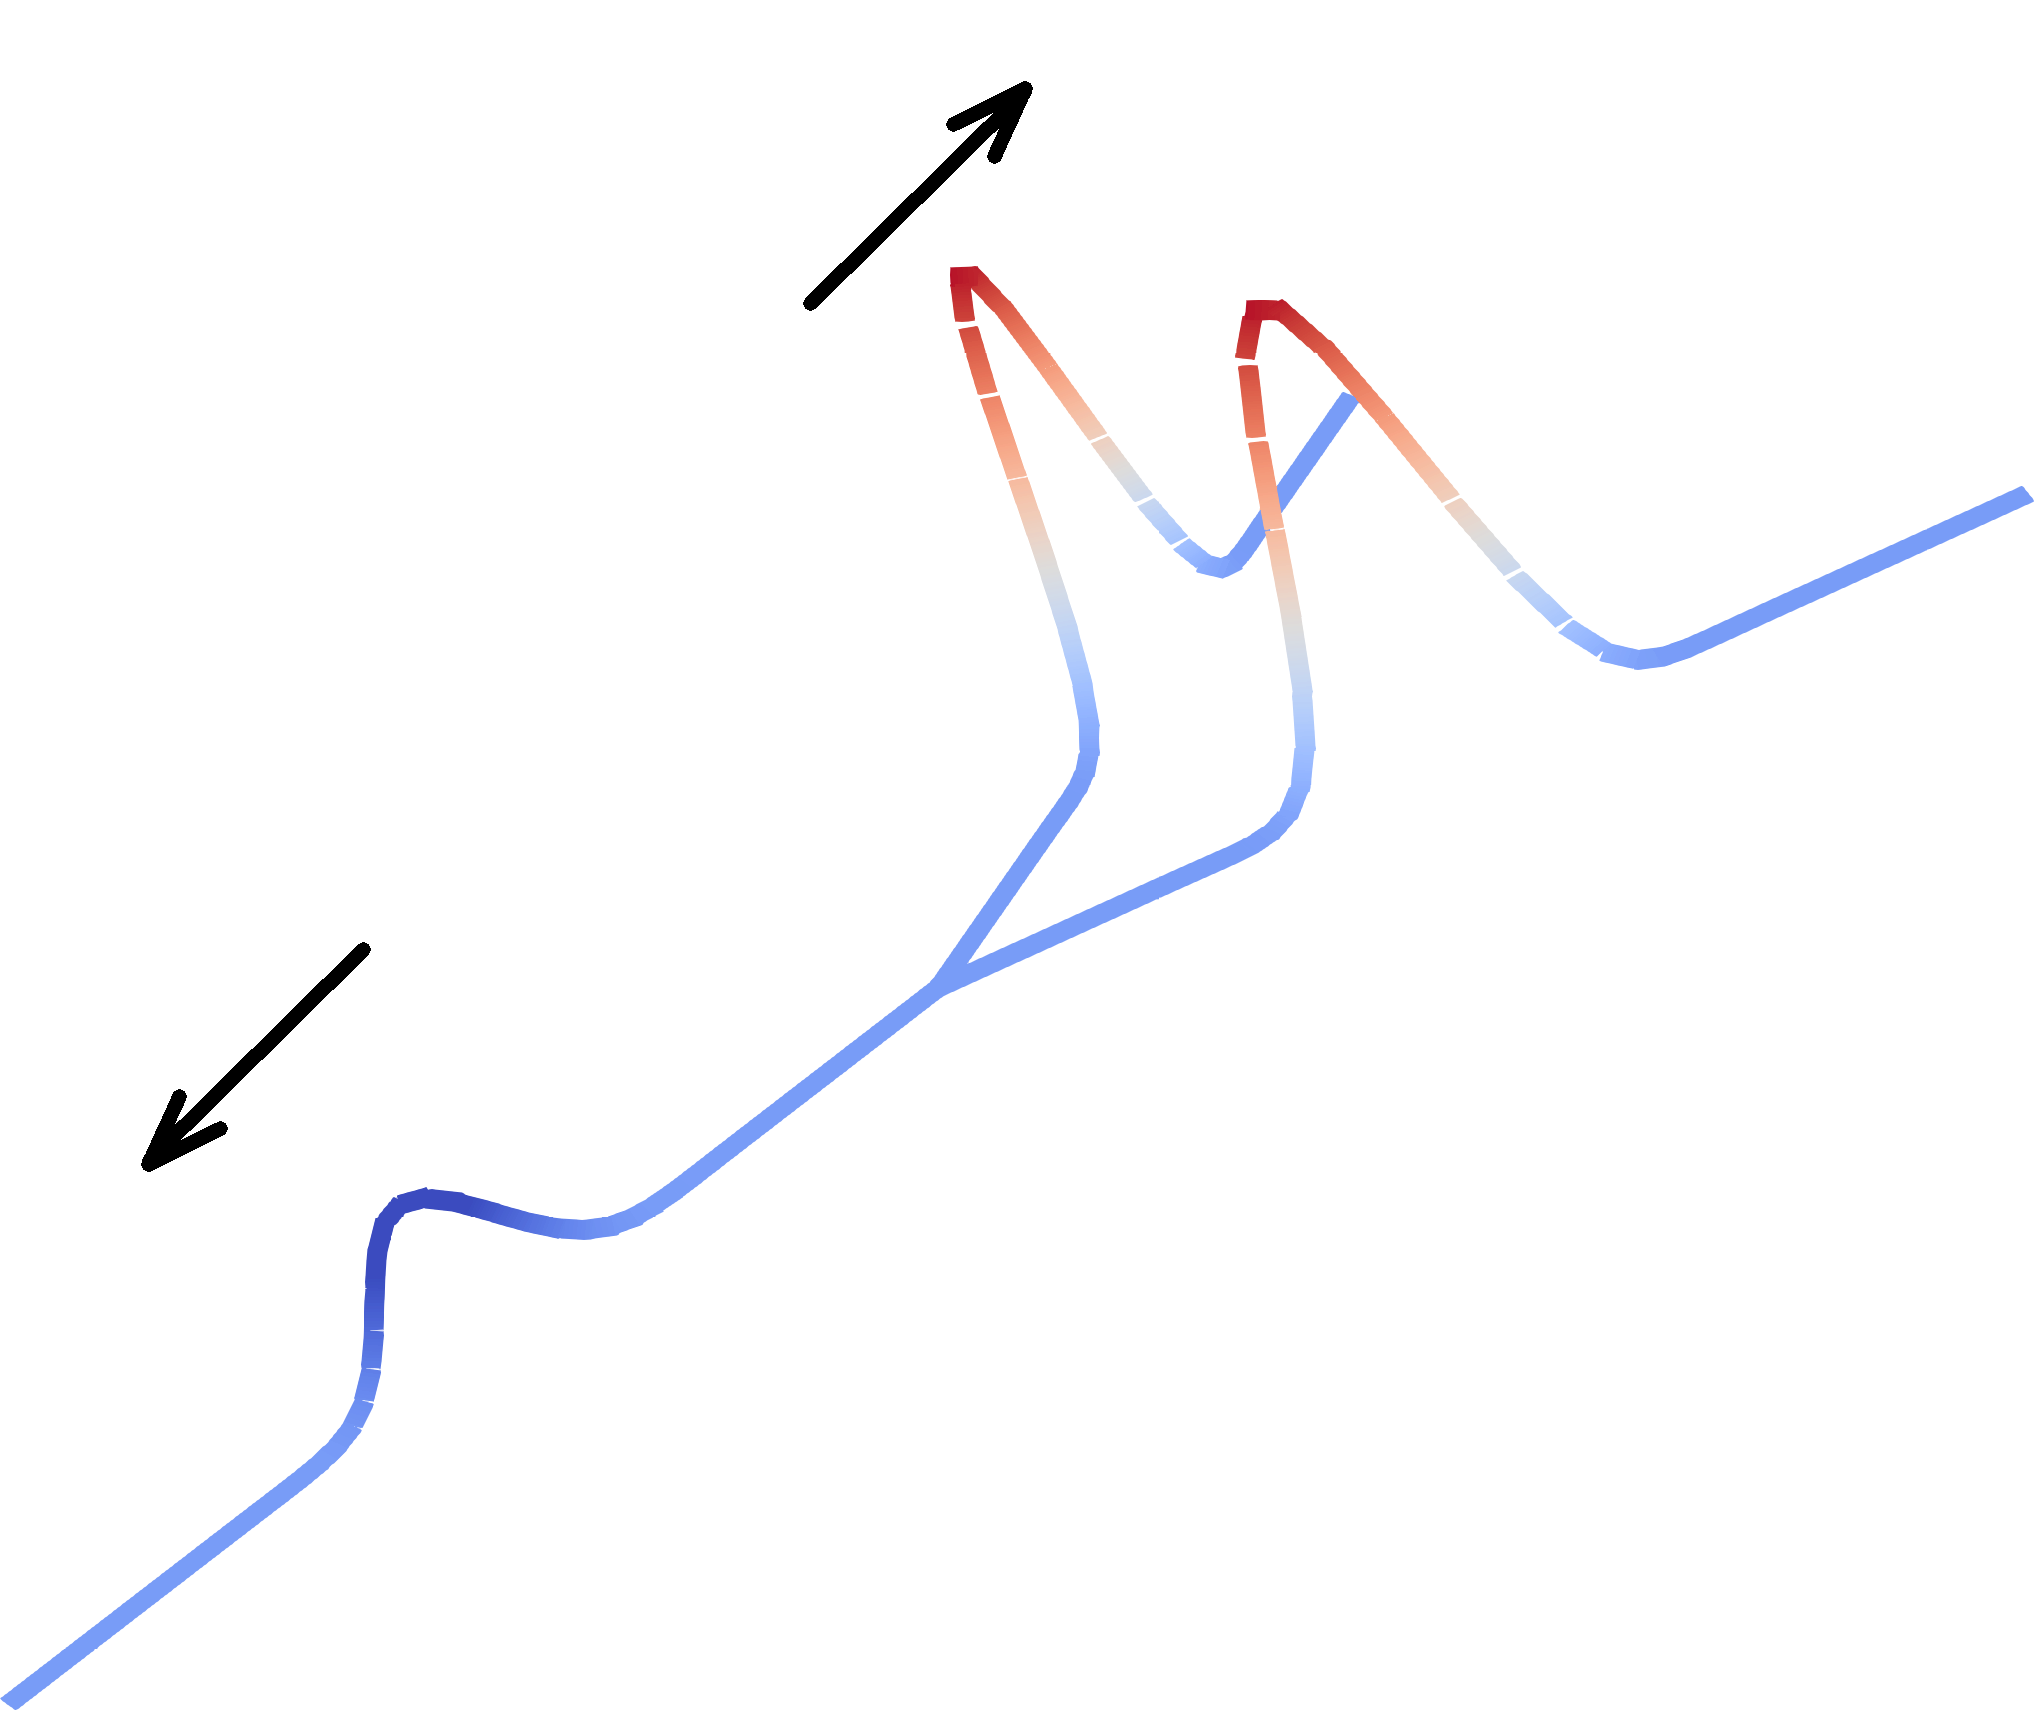
\includegraphics[width=0.4\linewidth]{prob4_time/p2.png}
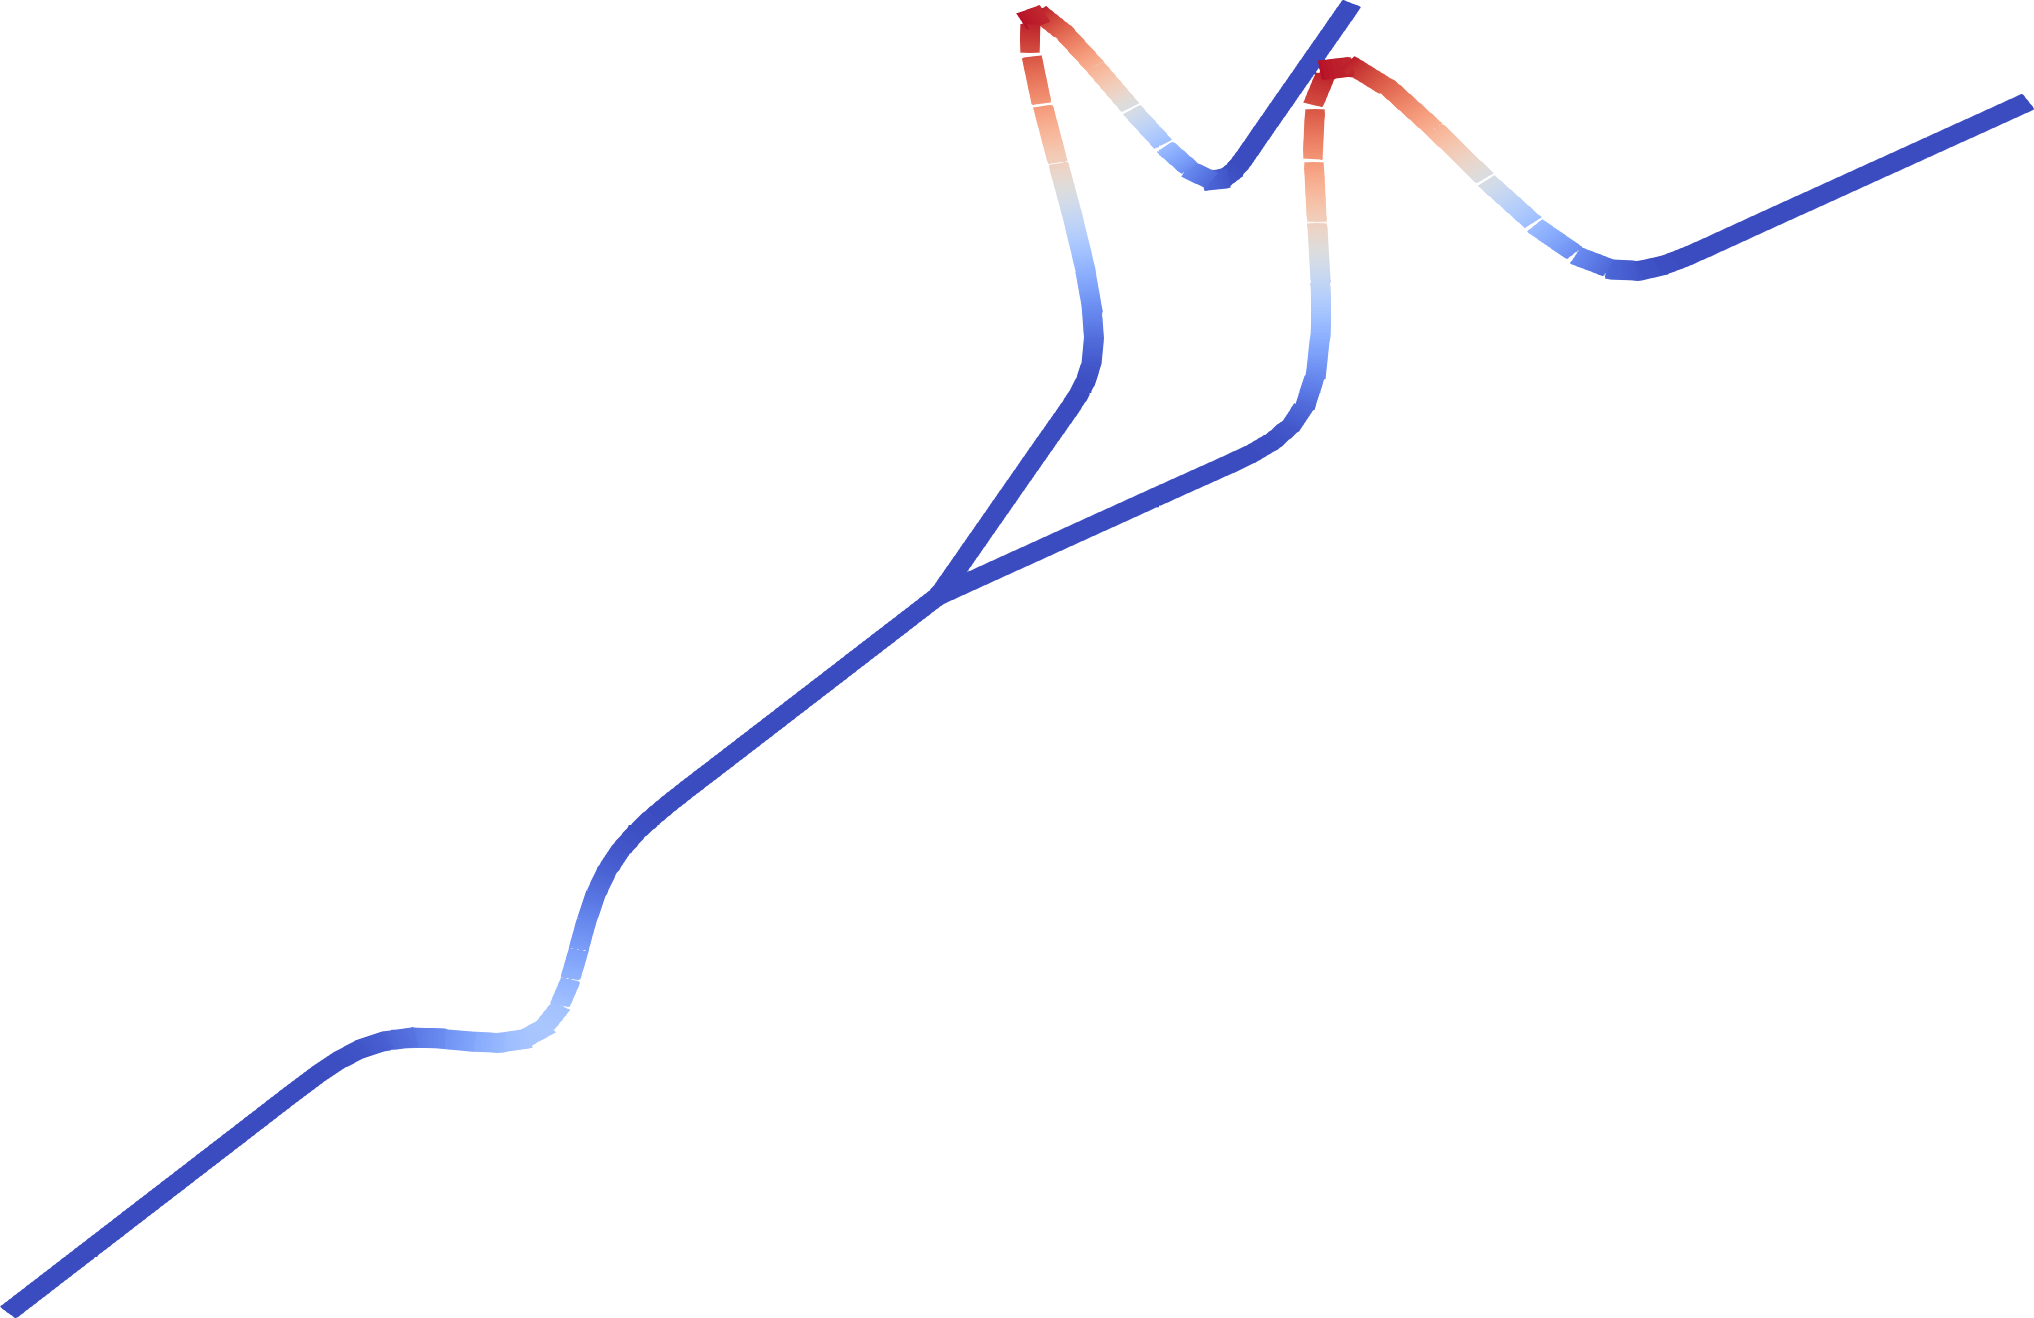
\includegraphics[width=0.4\linewidth]{prob4_time/v2.png}
\caption{$t=0.3$}\label{fig:prob4_pv_c}
\end{subfigure}\\
\caption{Значение давления (слева) и скорости (справа) на различные моменты времени}\label{fig:prob4_pv}
\end{figure}

\begin{figure}[h!]
\begin{subfigure}{1.0\linewidth}\centering
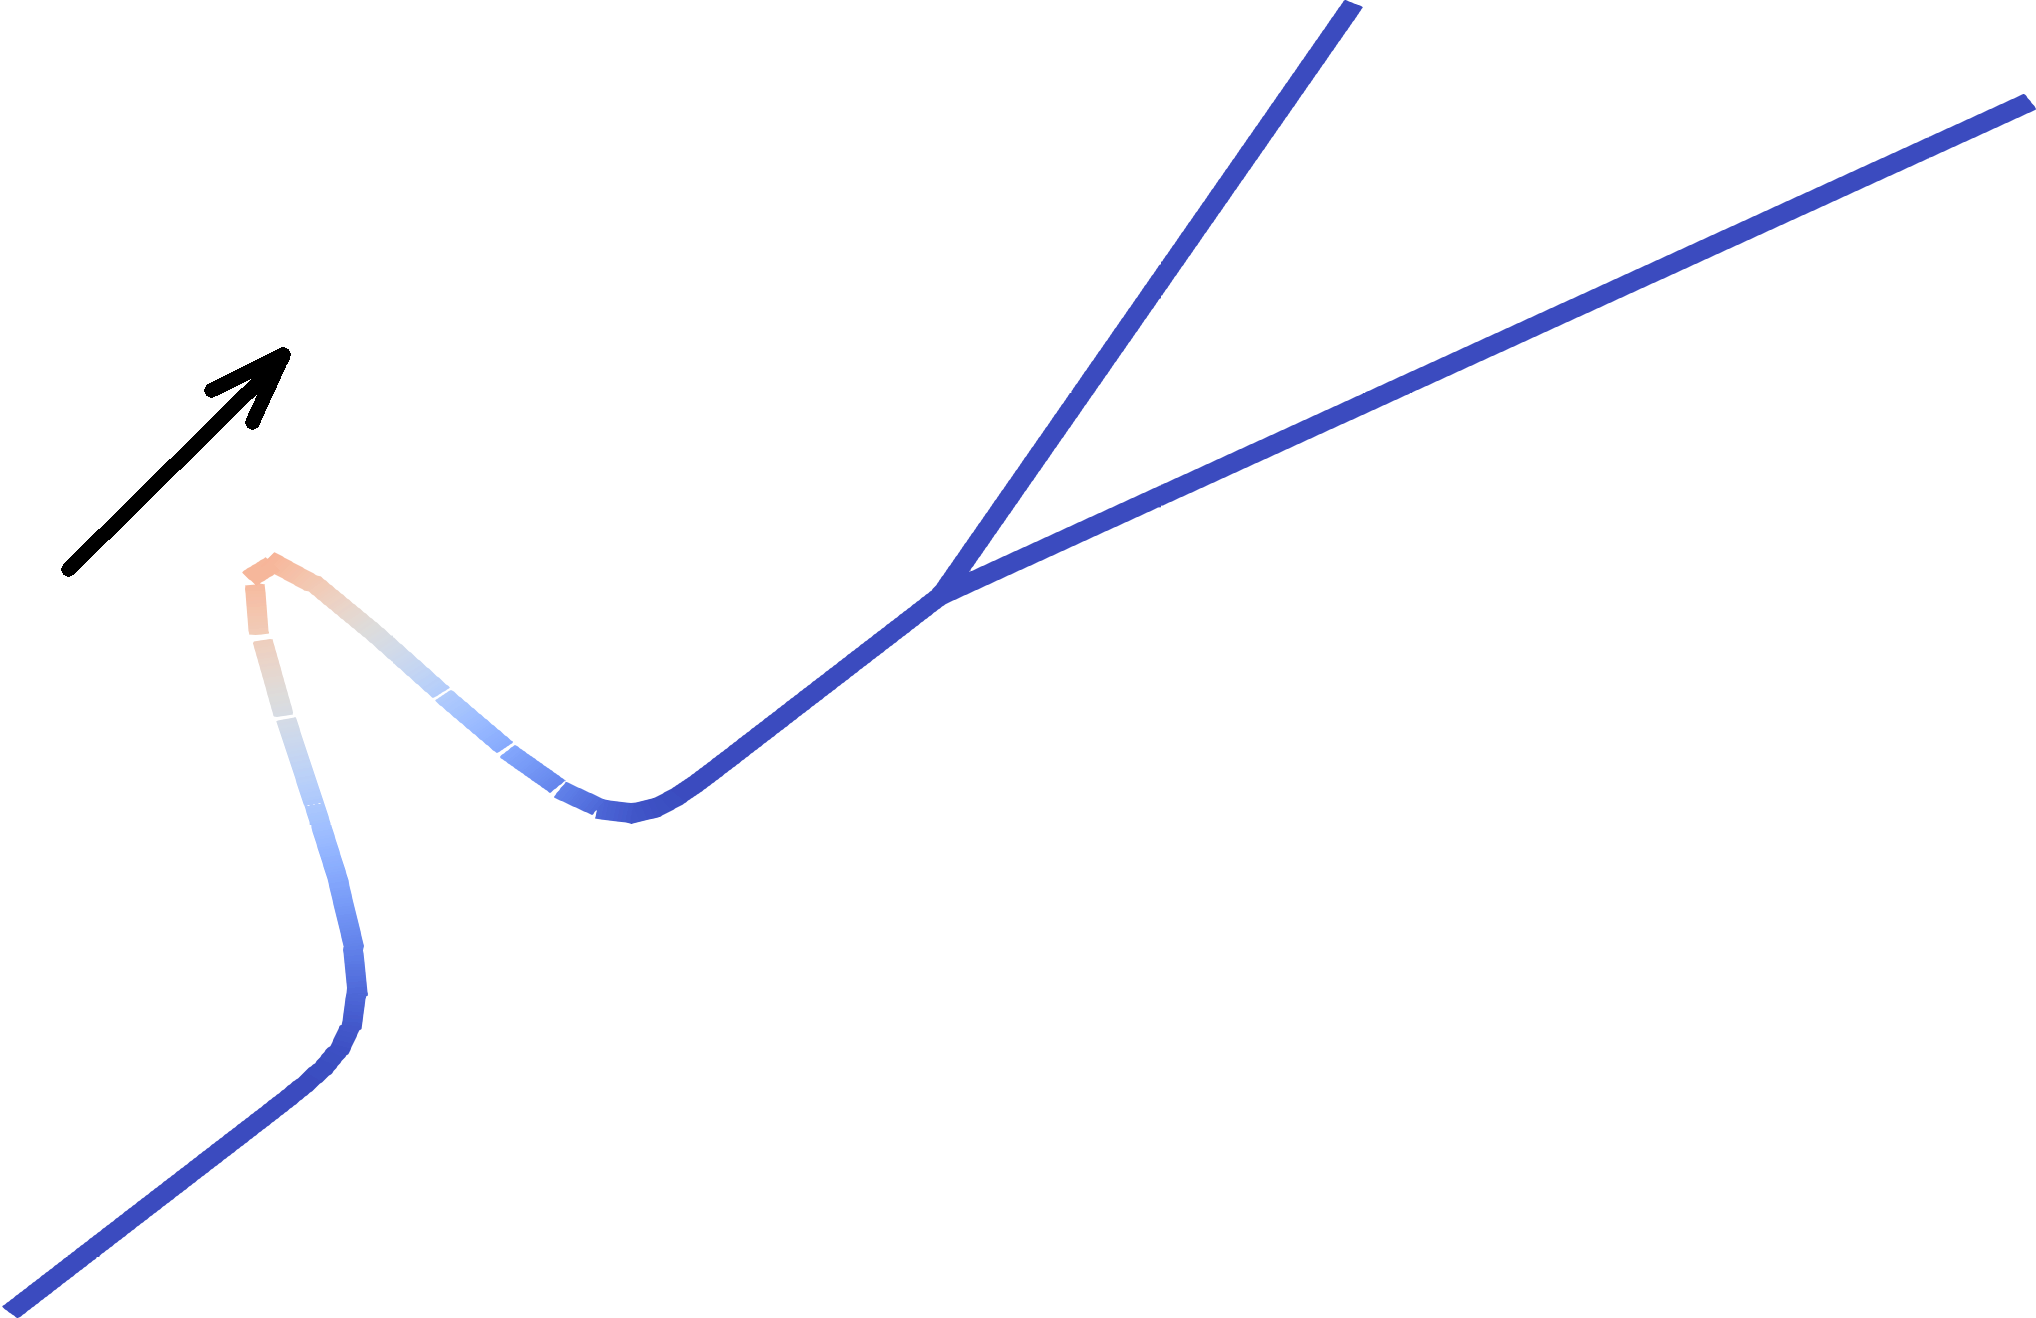
\includegraphics[width=0.4\linewidth]{prob4_time/w1_0.png}
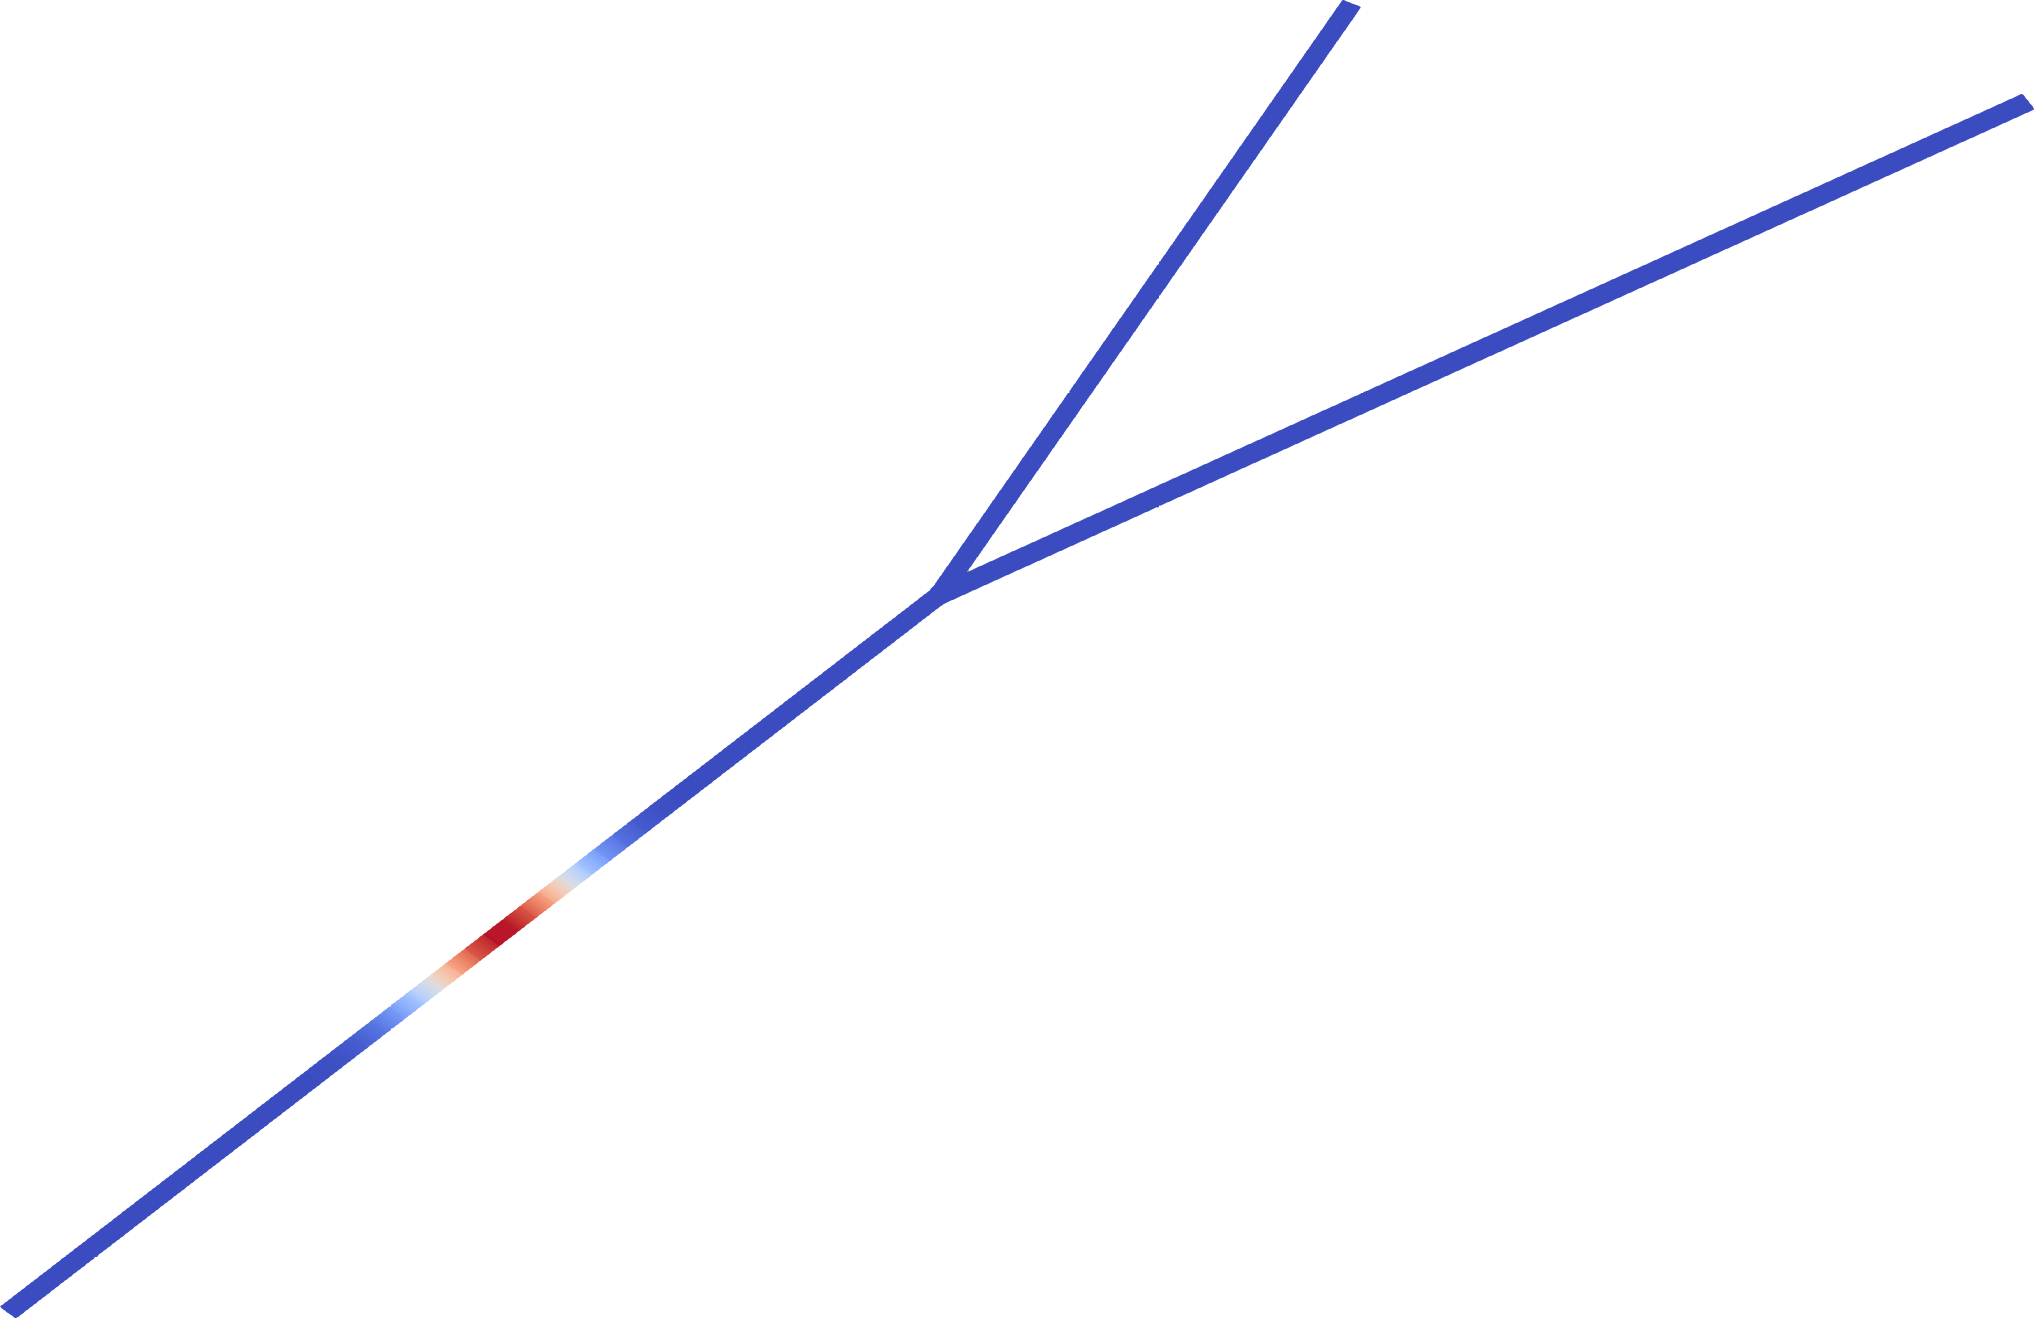
\includegraphics[width=0.4\linewidth]{prob4_time/w2_0.png}
\caption{$t = 0.13$}\label{fig:prob4_w12_a}
\end{subfigure} \\
\hfill \\
\hfill \\
\begin{subfigure}{1.0\linewidth}\centering
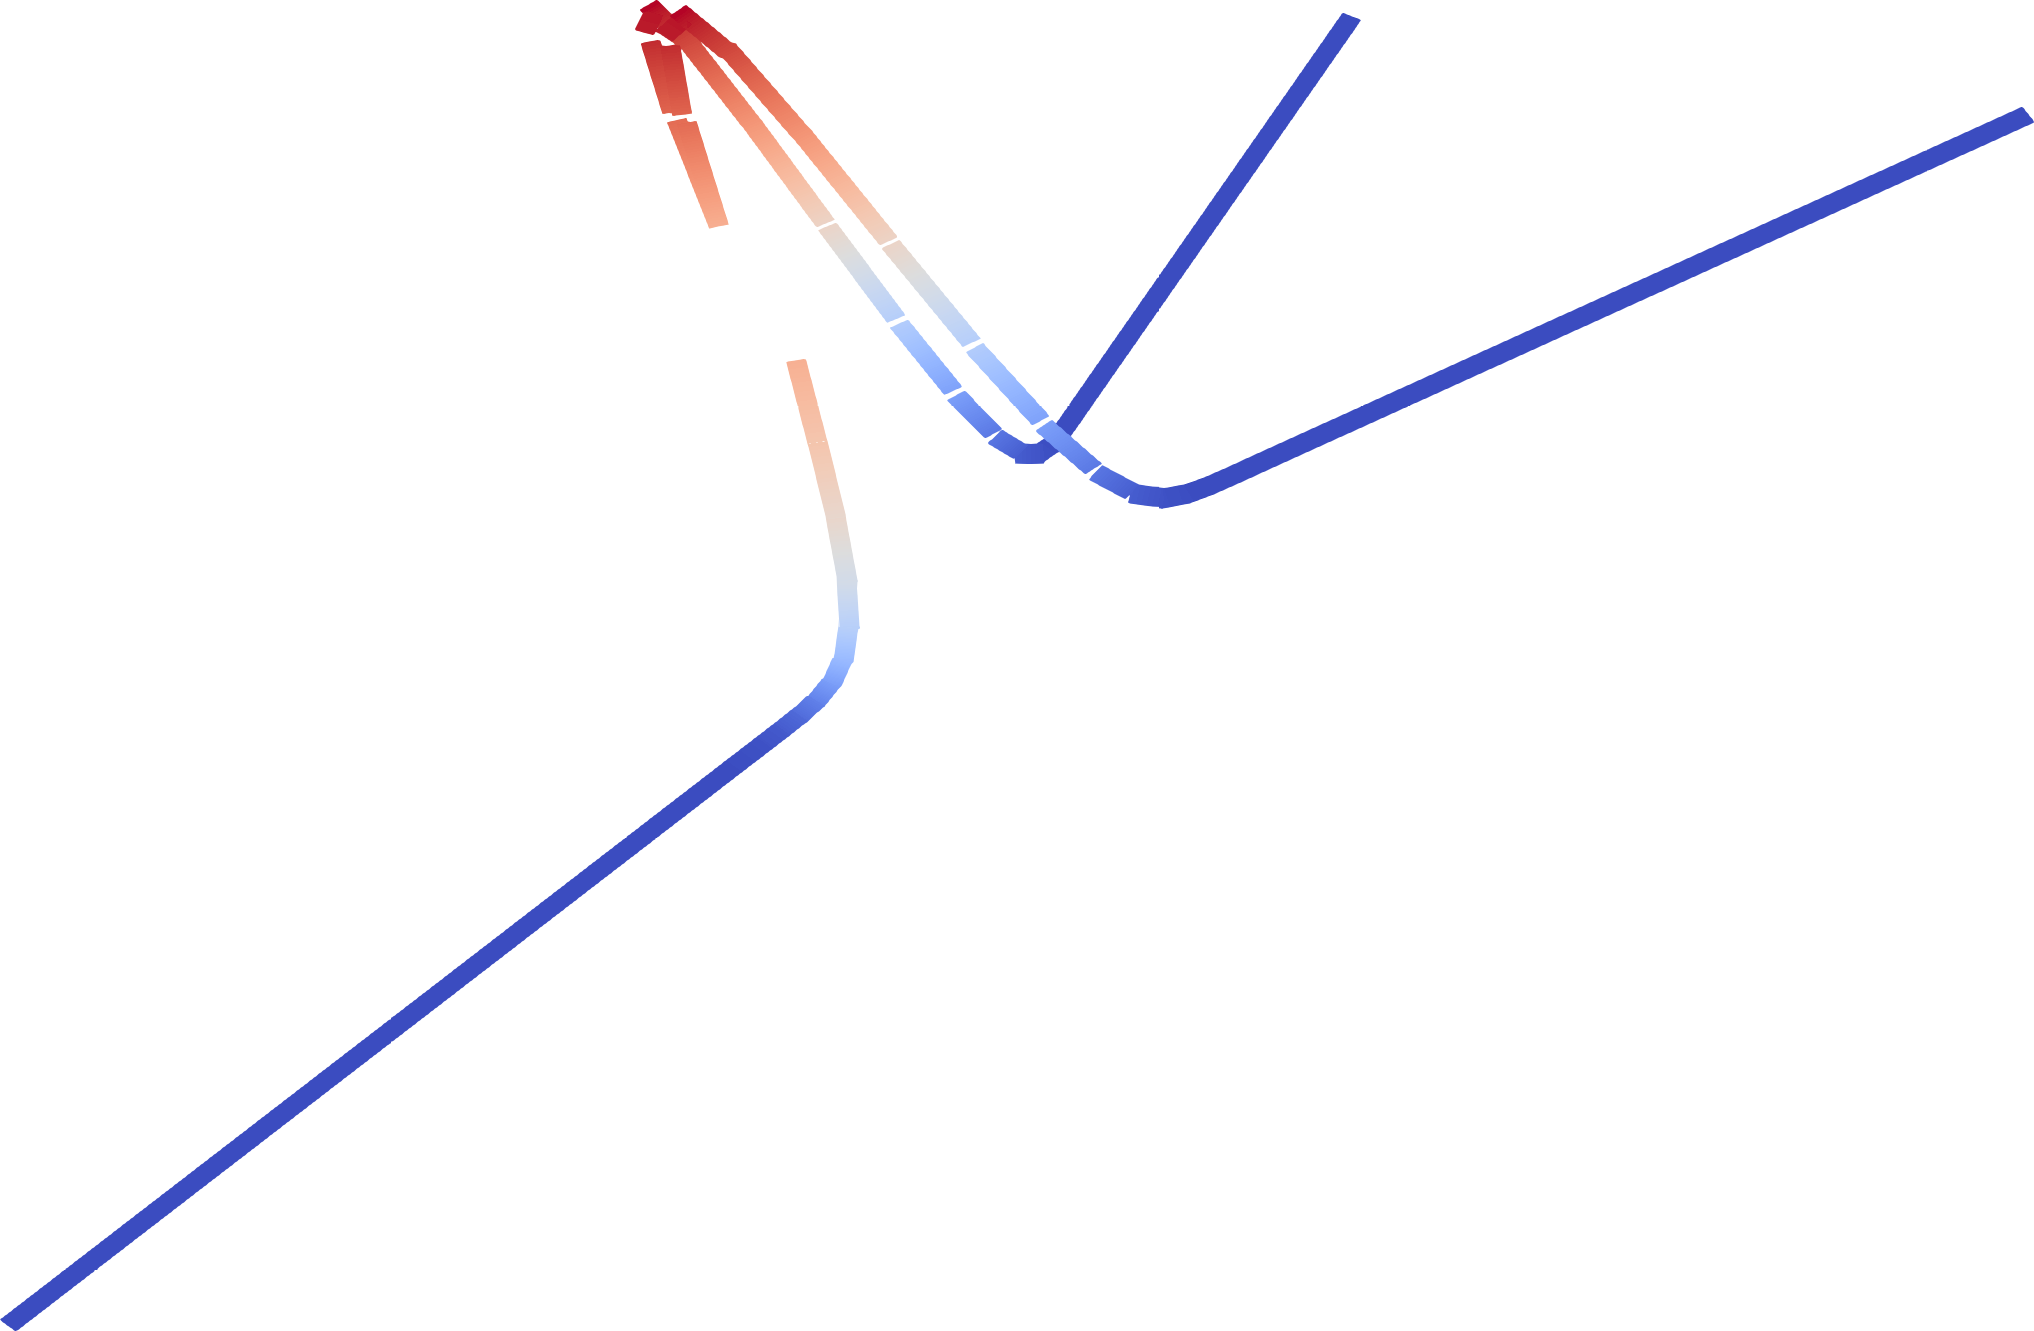
\includegraphics[width=0.4\linewidth]{prob4_time/w1_1.png}
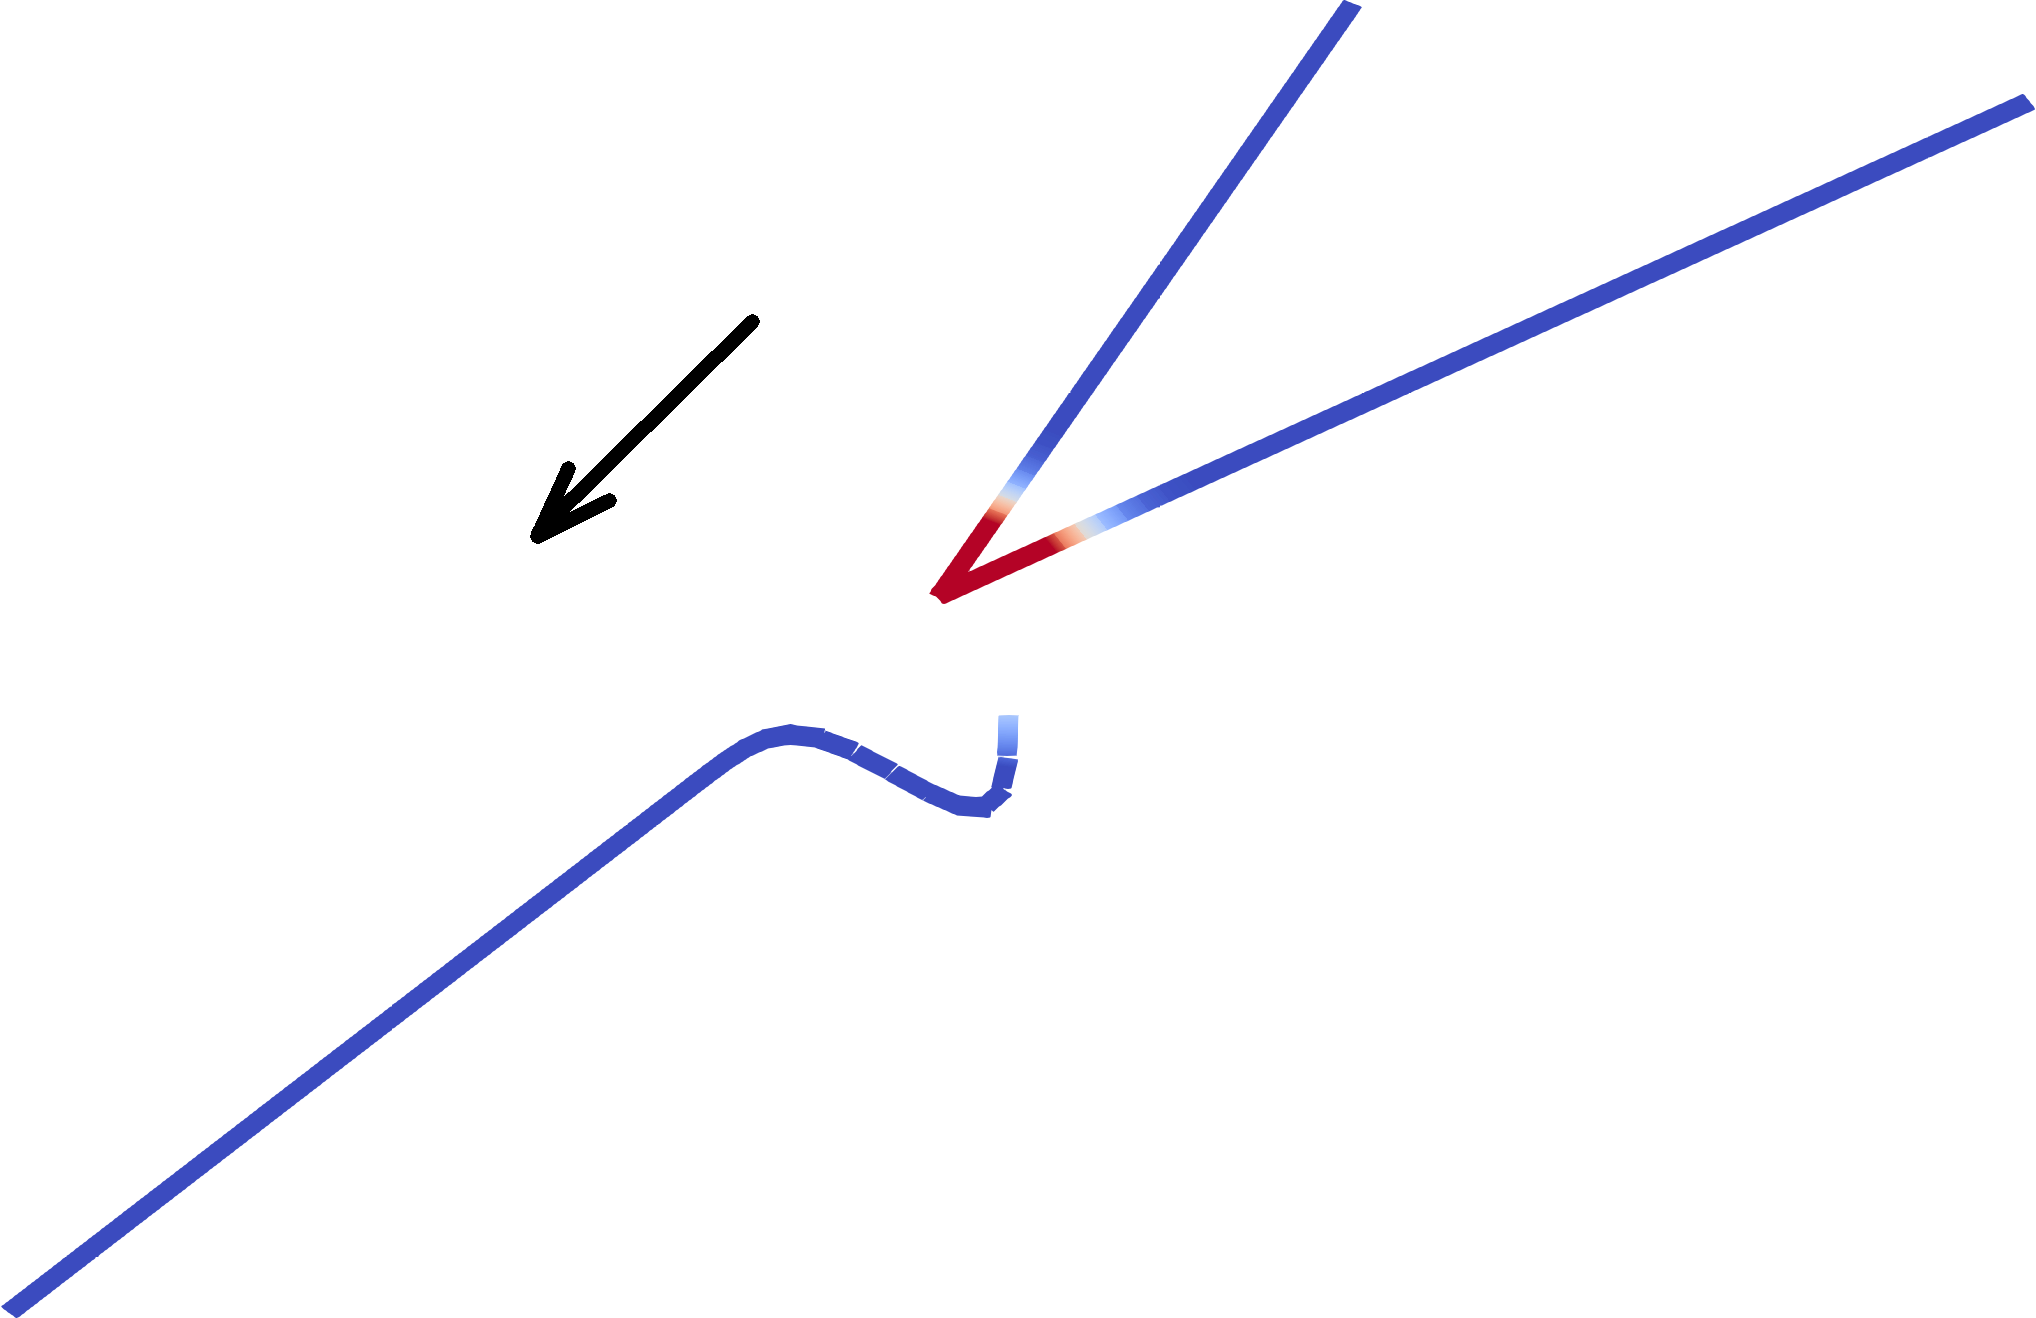
\includegraphics[width=0.4\linewidth]{prob4_time/w2_1.png}
\caption{$t = 0.22$}\label{fig:prob4_w12_b}
\end{subfigure}\\
\hfill \\
\hfill \\
\begin{subfigure}{1.0\linewidth}\centering
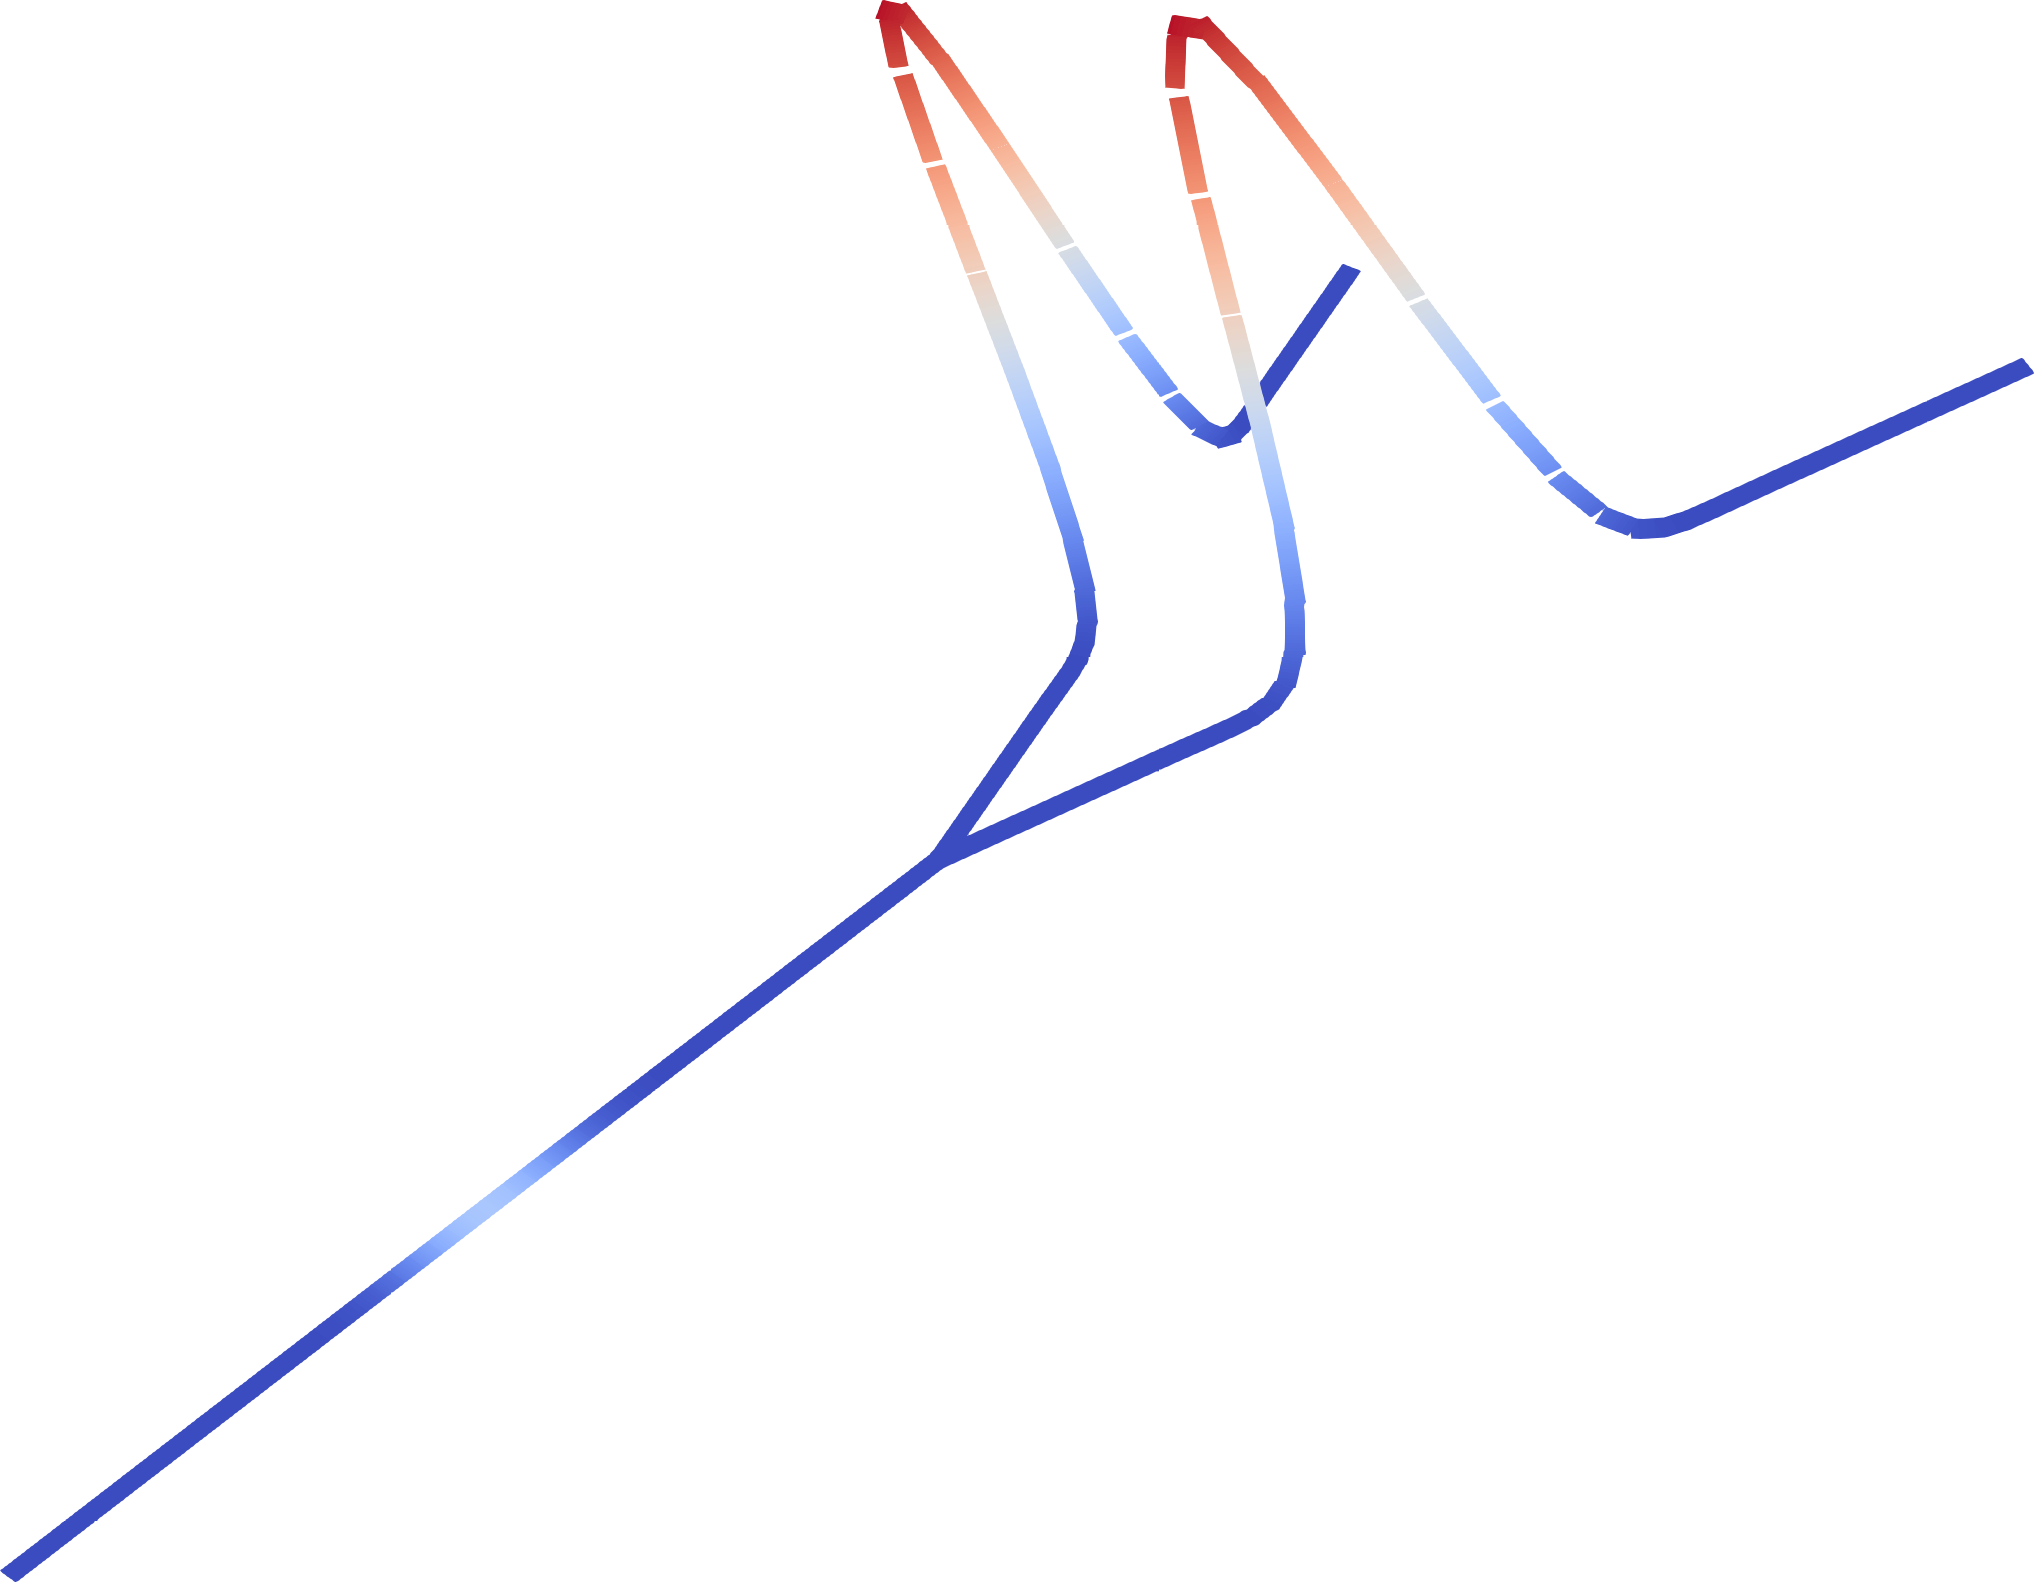
\includegraphics[width=0.4\linewidth]{prob4_time/w1_2.png}
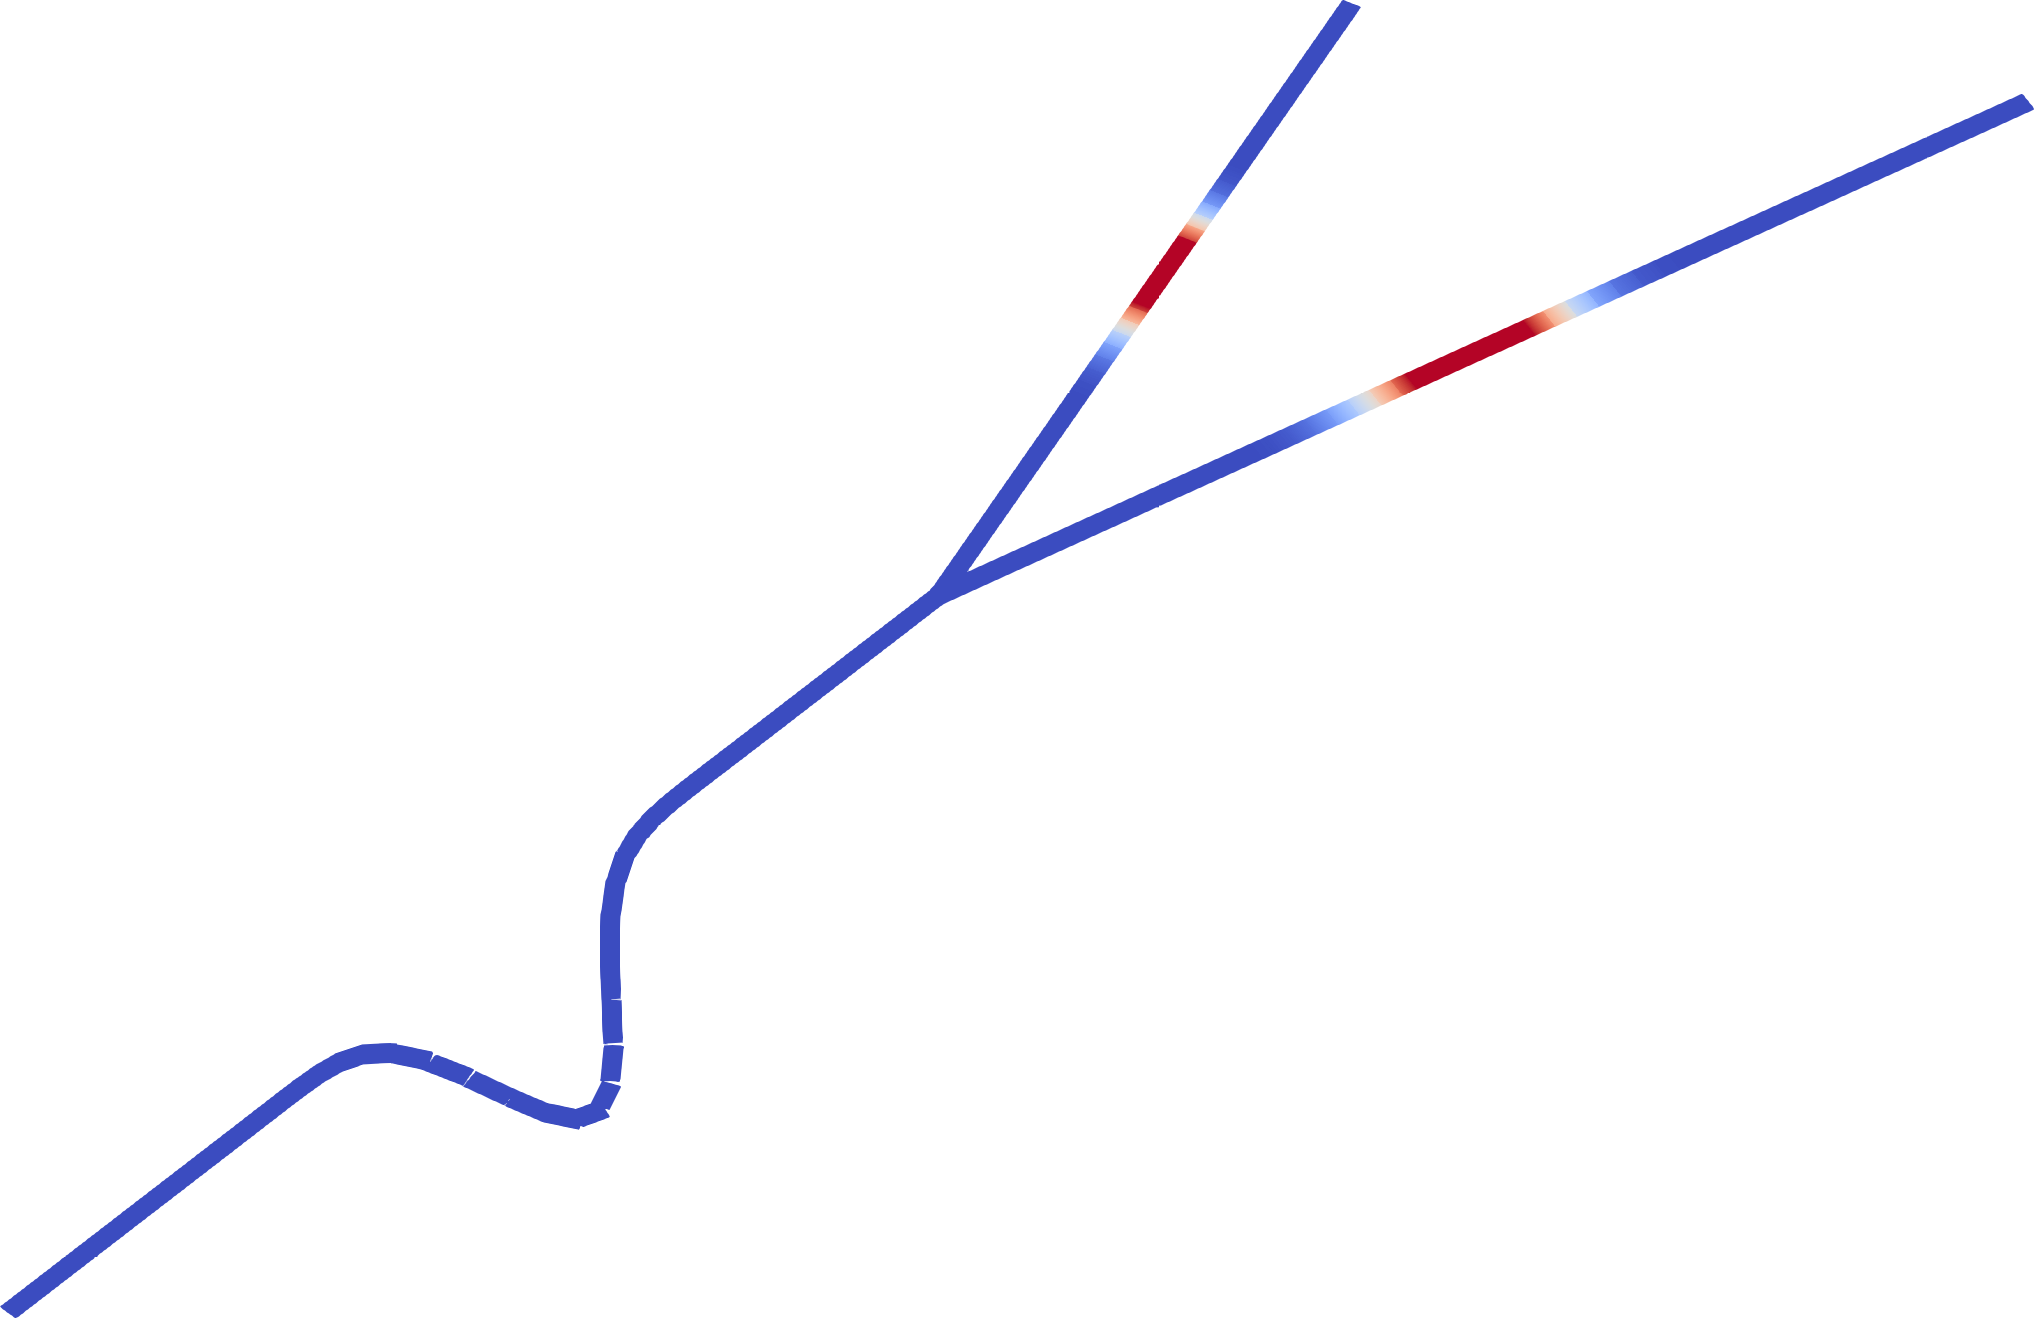
\includegraphics[width=0.4\linewidth]{prob4_time/w2_2.png}
\caption{$t=0.3$}\label{fig:prob4_w12_c}
\end{subfigure}\\
\caption{Значение переменной $w_1$ (слева) и $w_2$ (справа) на различные моменты времени}\label{fig:prob4_w12}
\end{figure}

Чтобы отделить поступательные волны от возвратных
был произведён пересчёт расчётных параметров
в переменные Римана $w_1$, $w_2$.
Их эволюция представлена на рис.~\ref{fig:prob4_w12}.
Как и следует из математического смысла этих переменных, каждая
из них содержит волны только одного направления.
Видно, что волна $w_2$ формируется
в момент, когда поступательная волна $w_1$
достигает точки разветвления (рис.~\ref{fig:prob4_w12_b}),
после чего волны $w_1$  и $w_2$ двигаются в противоположенных направлениях (рис.~\ref{fig:prob4_w12_c}).

\begin{figure}[h!]
\begin{subfigure}{0.5\linewidth}\centering
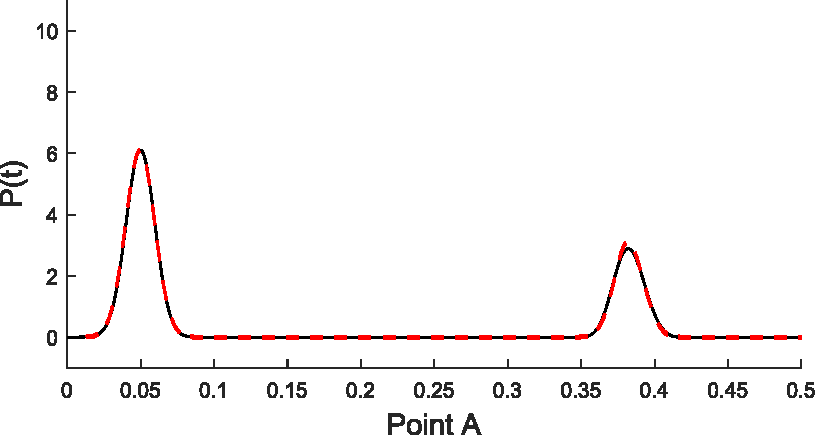
\includegraphics[width=0.9\linewidth]{problem4_pA1.pdf}
%\caption{}\label{fig:prob4_a}
\end{subfigure}%
\begin{subfigure}{0.5\linewidth}\centering
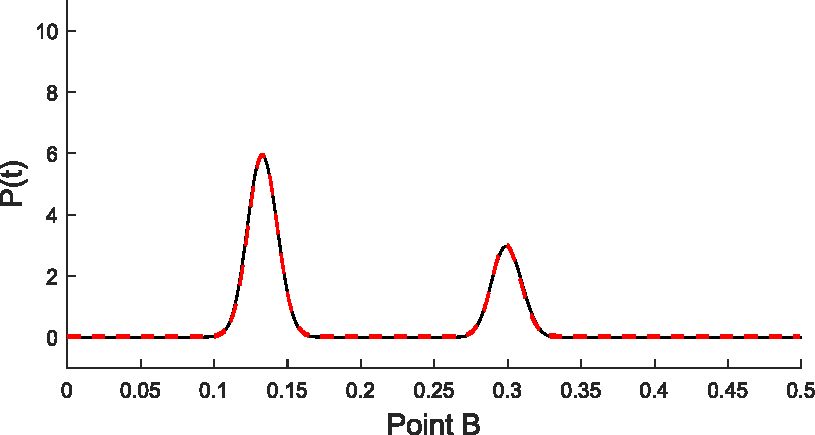
\includegraphics[width=0.9\linewidth]{problem4_pB1.pdf}
%\caption{}\label{fig:prob4_b}
\end{subfigure} \\
\hfill \\
\begin{subfigure}{0.5\linewidth}\centering
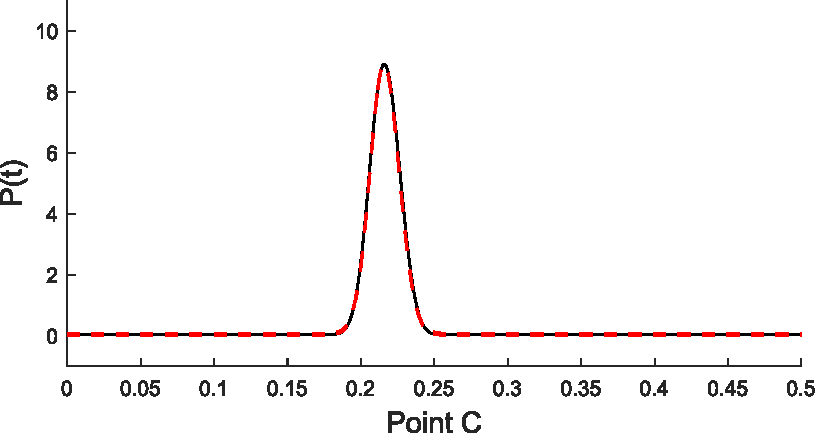
\includegraphics[width=0.9\linewidth]{problem4_pC1.pdf}
%\caption{}\label{fig:prob4_c}
\end{subfigure}%
\begin{subfigure}{0.5\linewidth}\centering
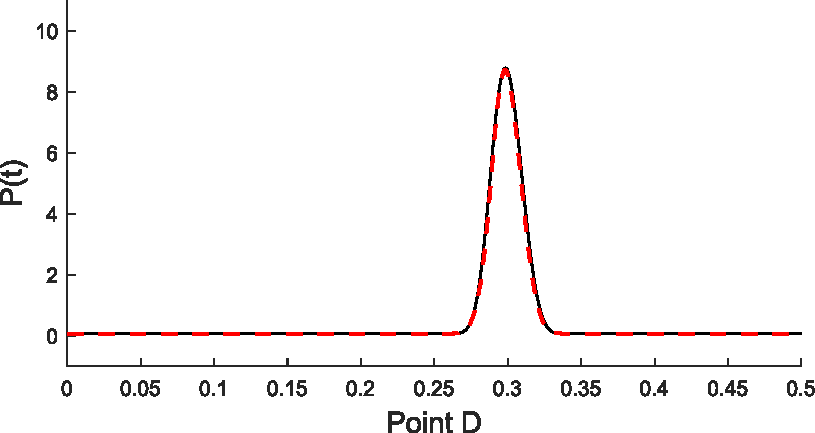
\includegraphics[width=0.9\linewidth]{problem4_pD1.pdf}
%\caption{}\label{fig:prob4_d}
\end{subfigure}\\
\hfill \\
\begin{subfigure}{0.5\linewidth}\centering
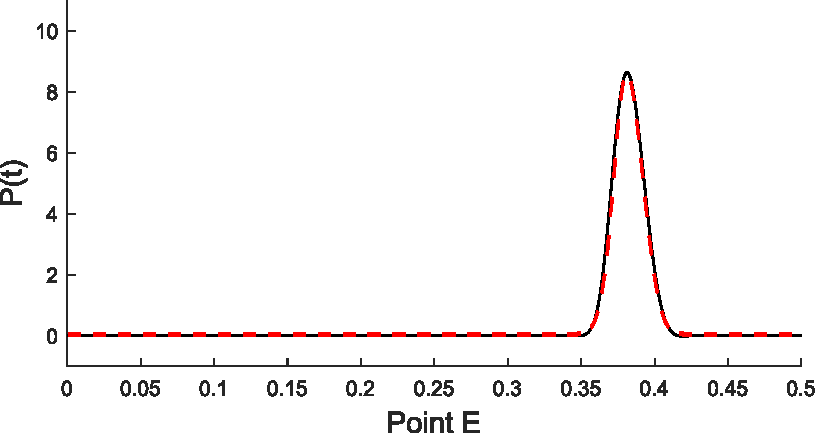
\includegraphics[width=0.9\linewidth]{problem4_pE1.pdf}
%\caption{}\label{fig:prob4_e}
\end{subfigure}%
\caption{Сравнение значения давления в контрольных точках. Сплошная линия -- наш расчёт, пунктирная -- результаты~\cite{Xiu:2007}}\label{fig:prob4_pt}
\end{figure}

Для сравнение полученных в результате наших расчётов данные с результатами из работы~\cite{Xiu:2007} 
были построены графики значения давления в контрольных точках (расположение контрольных точек смотри на рис.~\ref{fig:prob4_pv_a}).
Наложение графиков, демонстрирующее хорошее совпадение результатов, представлено на рис.~\ref{fig:prob4_pt}.
На графиках для точек A и B видно, что через соответствующие контрольные точки проходит
две волны. Сначала поступательная, потом отражённая возвратная.
Тут же следует отметить, что отсутствие других возмущений
говорит о корректной работе неотражающих граничных условий.


\subsection{Течение в системе сосудов}
Для иллюстрации применения численного метода
рассмотрим задачу о течении в системе из семи сосудов, представленных на рис.~\ref{fig:seven_vessel}.
\begin{figure}[h!]
\centering
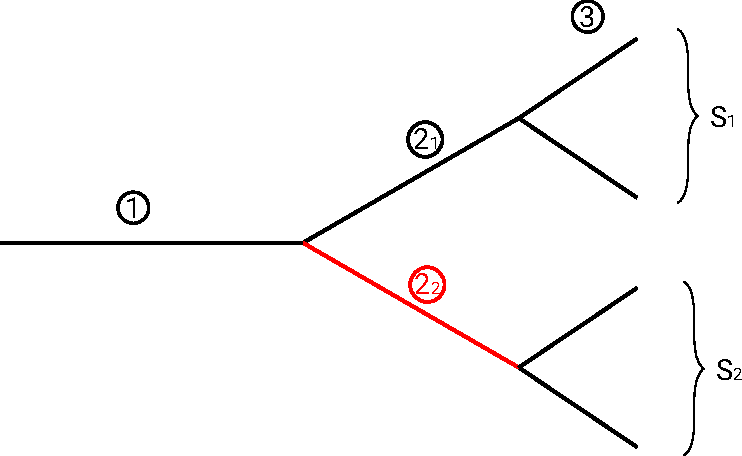
\includegraphics[width=0.6\linewidth]{seven_vessel.pdf}
\caption{Система из семи сосудов}\label{fig:seven_vessel}
\end{figure}%

Сосуды поделены на три группы: в группе $1$ один крупный сосуд,
 в группе $2$ два средних сосуда и в группе $3$ четыре малых сосуда.
Базовые свойства этих сосудов приведены в таблице \cref{tab:prob5_vessel}.

\begin{equation}
\label{tab:prob5_vessel}
\begin{array}{l|c|c|c}
\text{параметр}  & \text{сосуд 1} & \text{сосуды 2} & \text{сосуды 3}\\
\hline
\text{длина, м} & 1.0 & 0.8 & 0.5\\
\hline
R\text{, мм} & 5.0 & 4.0 & 3.0\\
\hline
E\text{, МПа} & \multicolumn{3}{c}{1.0}\\
\hline
h\text{, мм} & \multicolumn{3}{c}{0.15}\\
\hline
\rho\text{, кг/м\textsuperscript{3}} & \multicolumn{3}{c}{1050}\\
\hline
\mu\text{, Па с} & \multicolumn{3}{c}{0}\\
\hline
\end{array}
\end{equation}

Упругие свойства нижнего из промежуточных сосудов (обозначен $2.2$ на рисунке~\ref{fig:seven_vessel})
в зависимости от варианта расчёта изменяются согласно вариантам, представленным в таблице~\ref{tab:prob5_case}.
\begin{equation}
\label{tab:prob5_case}
\begin{array}{l|c|c|c|c}
\text{параметр}  & \text{вариант I} & \text{вариант II} & \text{вариант III} & \text{вариант IV}\\
\hline
R\text{, мм} & 4.0 & 4.0 & 4.0/\sqrt{2} & 4.0/\sqrt{2} \\
\hline
E\text{, МПа} & 1.0 & 10 & 1 & 10 \\
\hline
\end{array}
\end{equation}
Такие изменения характерны для склеротических поражений сосудов, при которых
увеличивается жёсткость стенки и уменьшается эффективный радиус сосуда.
Вариант I будем считать базовым, в варианте II увеличен модуль упругости сосуда,
в варианте III уменьшен радиус сосуда, вариант IV является суммой изменений из вариантов II и III.

На входе устанавливается периодическое значение расхода $q_{in}(t)$
с максимальным значением в $20$мл/сек.
Рассматривается два периода, соответствующие частоте сердцебиения \gls{bpm} в 60 (спокойный пульс) и 180 (высокий пульс) ударов в минуту.
В качестве выходного параметра мониторятся выходное значение расхода в сечениях, обозначенных на рис.~\ref{fig:seven_vessel} как $S_1$ (неповрежденная сторона системы)
и $S_2$ (повреждённая сторона системы).

Результаты для значения $bpm=60$ приведены на рис.~\ref{fig:prob5_q1}, а для $bpm=180$ -- на рис.~\ref{fig:prob5_q2}.
На рис.~\ref{fig:prob5_time} приведено значение скорости течения на различные моменты времени.
Видно, что оба типа повреждения значительно уменьшают количество
жидкости, протекающей через повреждённую сторону, при этом также происходит
изменения величины расхода и для неповреждённой стороны. В частности, там наблюдаются потоки, текущие в обратном направлении ($u<0$).
Для $bpm=180$ качественная картина не меняется, но при этом перепады значений расходов между сечениями $S_1$ и $S_2$
кратно увеличивается.
Из этого можно сделать вывод, что негативные последствия, связанные с нарушением эластичности стенок сосудов, проявляет себя сильнее при
высоком пульсе.

\begin{figure}[h!]
\begin{subfigure}{0.5\linewidth}\centering
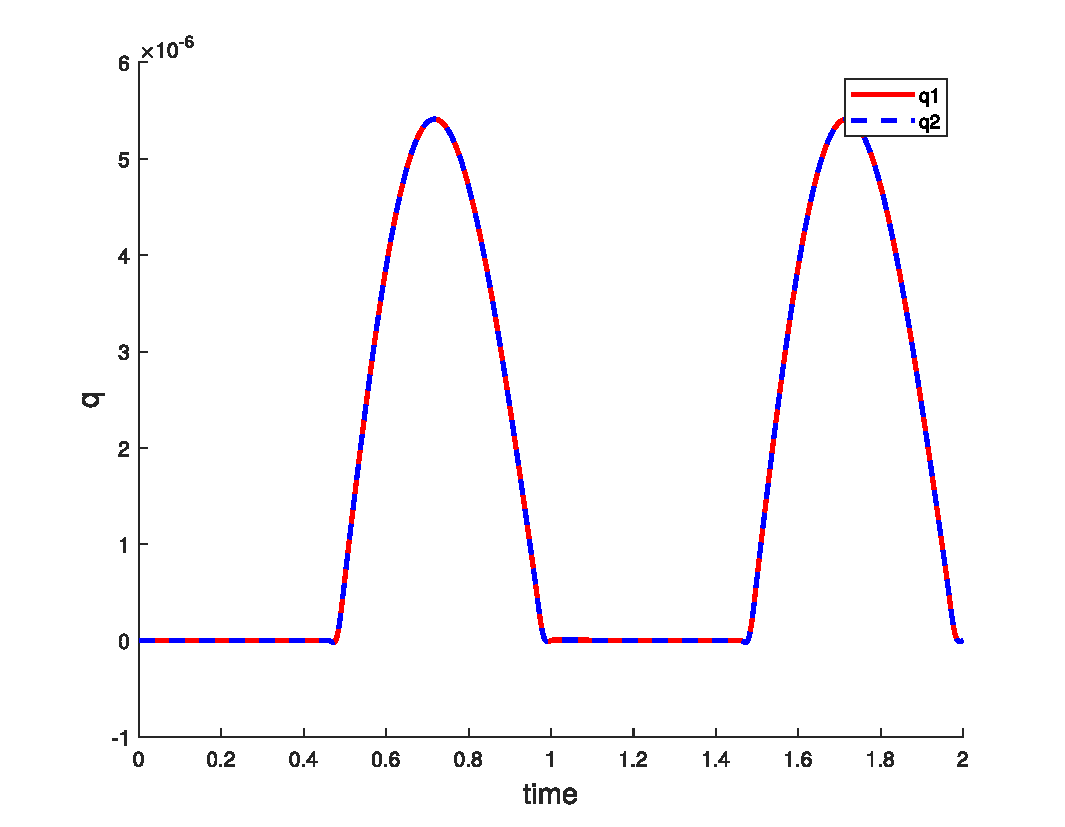
\includegraphics[width=0.9\linewidth]{q1_eq.pdf}
\caption{Вариант I}\label{fig:prob5_q1_eq}
\end{subfigure}%
\begin{subfigure}{0.5\linewidth}\centering
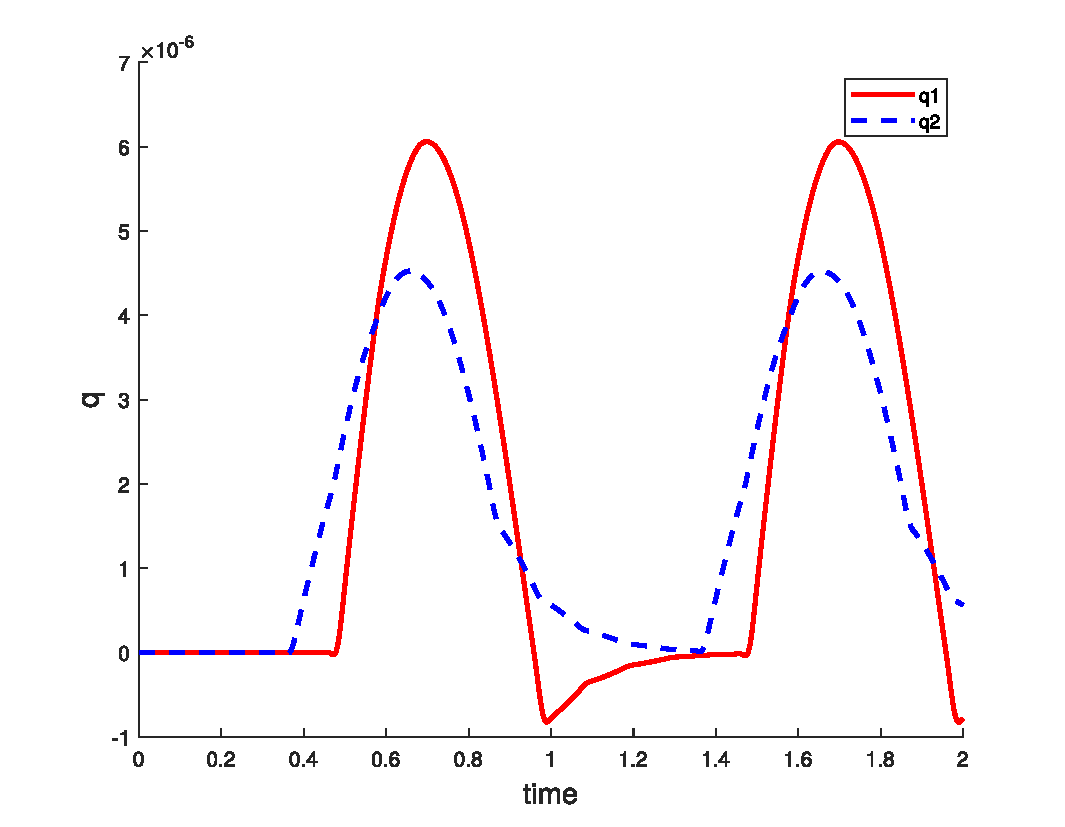
\includegraphics[width=0.9\linewidth]{q1_e10.pdf}
\caption{Вариант II}\label{fig:prob5_q1_e10}
\end{subfigure} \\
\hfill \\
\begin{subfigure}{0.5\linewidth}\centering
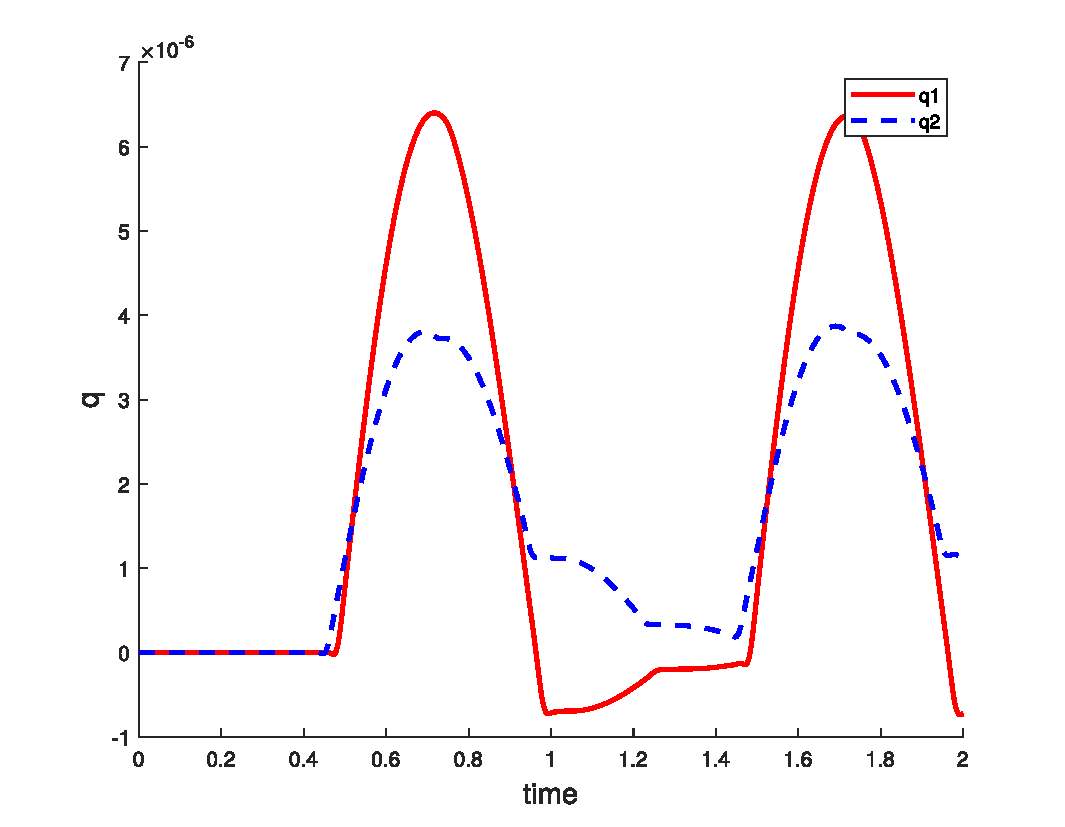
\includegraphics[width=0.9\linewidth]{q1_a2.pdf}
\caption{Вариант III}\label{fig:prob5_q1_a2}
\end{subfigure}%
\begin{subfigure}{0.5\linewidth}\centering
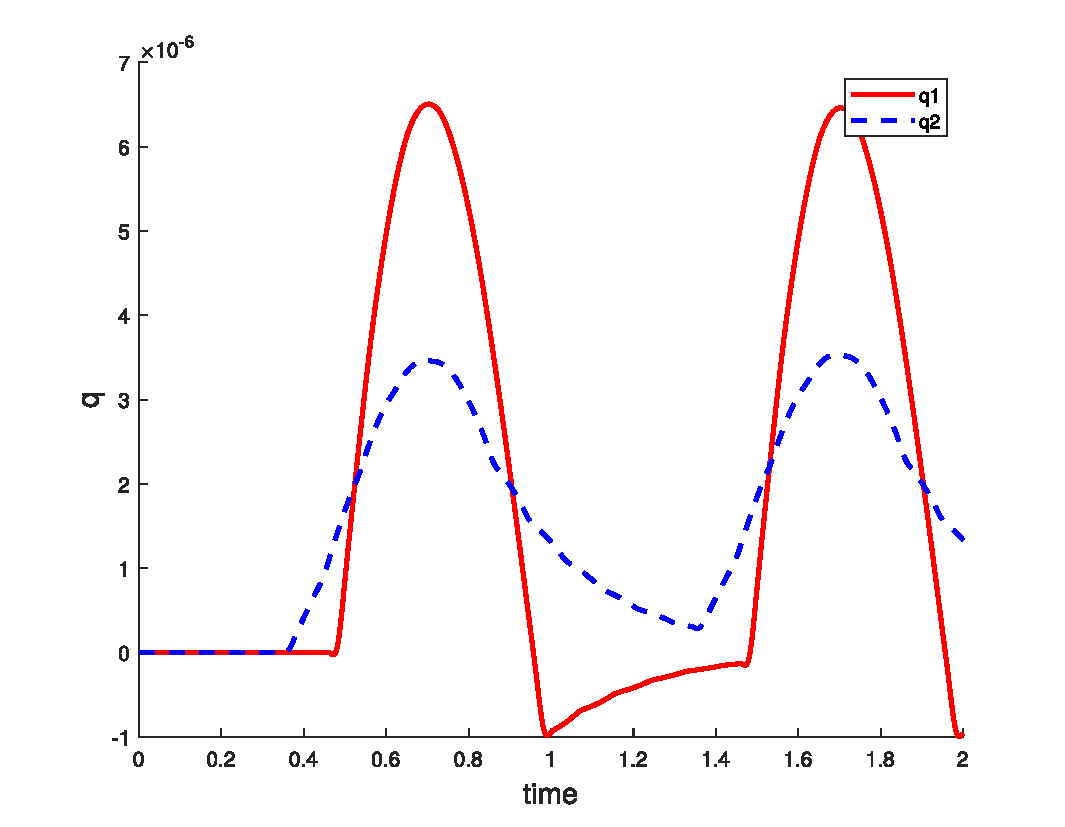
\includegraphics[width=0.9\linewidth]{q1_e10a2.pdf}
\caption{Вариант IV}\label{fig:prob5_a1_e10a2}
\end{subfigure}%
\caption{Значение расходов через сечения $S_1$ (красная линия) и $S_2$ (синяя линия) для различных способов повреждения сосудов, ведущих к $S_2$. Частота -- $bpm=60$}
\label{fig:prob5_q1}
\end{figure}

\begin{figure}[h!]
\begin{subfigure}{0.5\linewidth}\centering
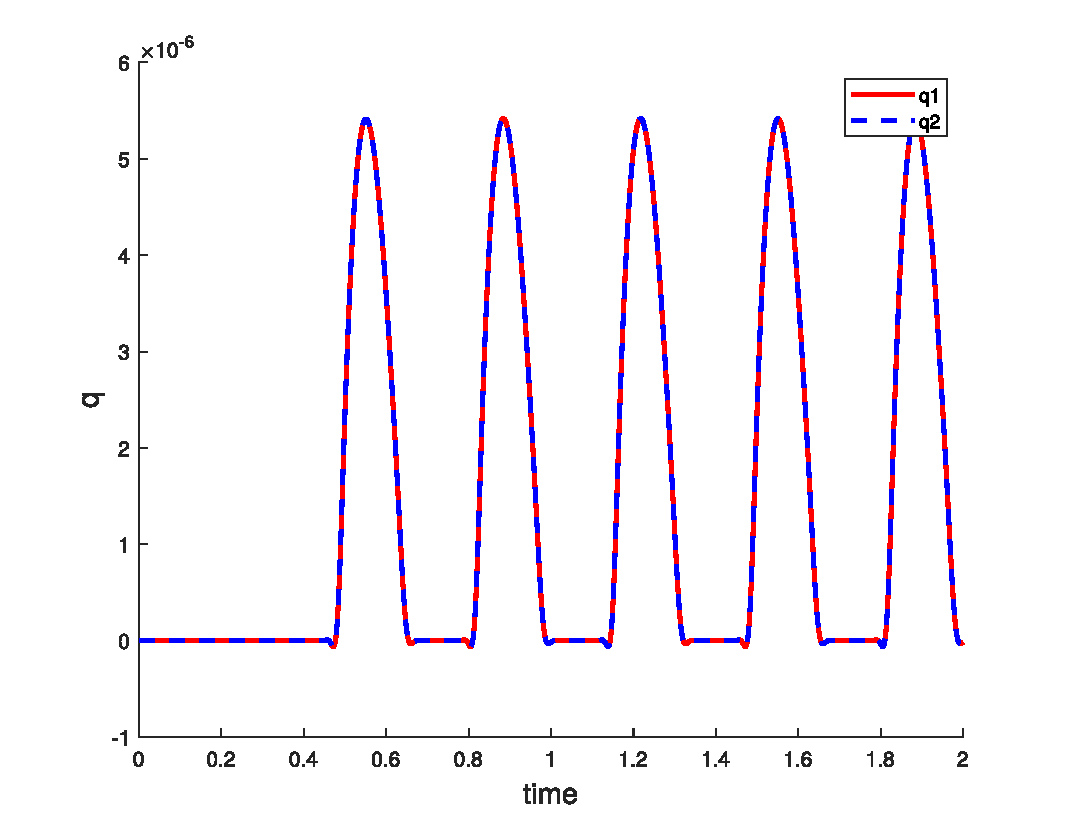
\includegraphics[width=0.9\linewidth]{q2_eq.pdf}
\caption{Вариант I}\label{fig:prob5_q2_eq}
\end{subfigure}%
\begin{subfigure}{0.5\linewidth}\centering
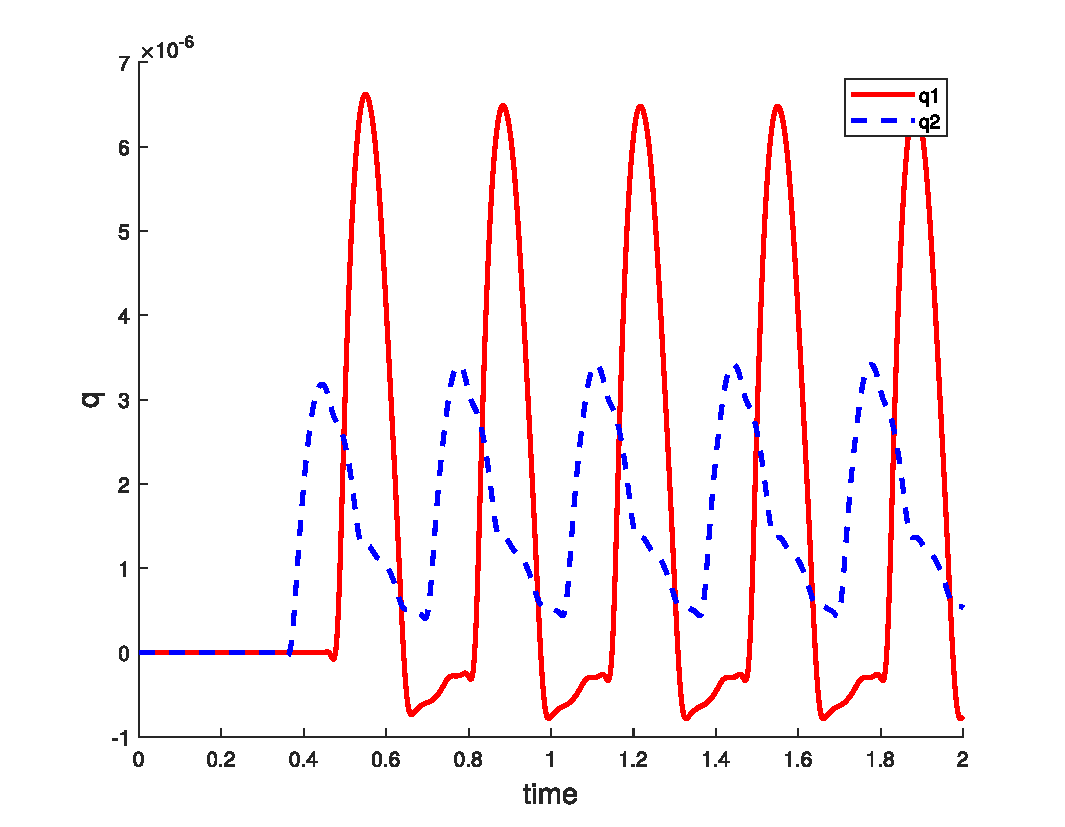
\includegraphics[width=0.9\linewidth]{q2_e10.pdf}
\caption{Вариант II}\label{fig:prob5_q2_e10}
\end{subfigure} \\
\hfill \\
\begin{subfigure}{0.5\linewidth}\centering
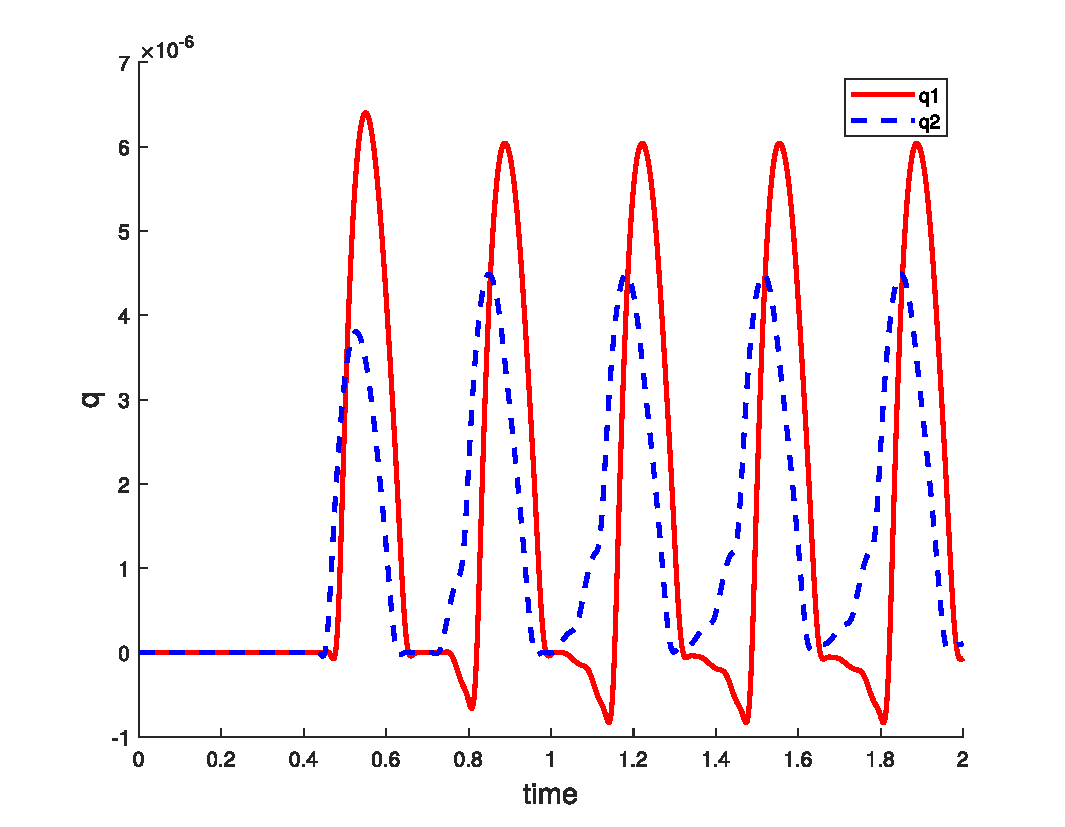
\includegraphics[width=0.9\linewidth]{q2_a2.pdf}
\caption{Вариант III}\label{fig:prob5_q2_a2}
\end{subfigure}%
\begin{subfigure}{0.5\linewidth}\centering
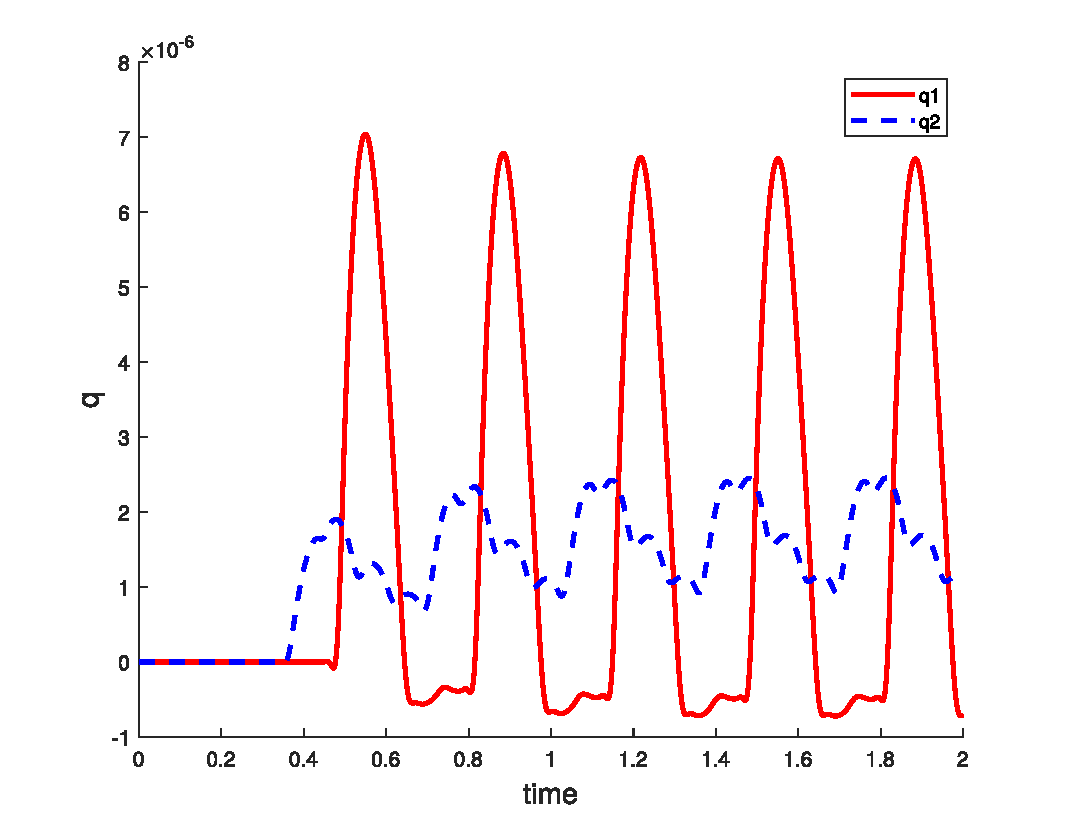
\includegraphics[width=0.9\linewidth]{q2_e10a2.pdf}
\caption{Вариант IV}\label{fig:prob5_a2_e10a2}
\end{subfigure}%
\caption{Значение расходов через сечения $S_1$ (красная линия) и $S_2$ (синяя линия) для различных способов повреждения сосудов, ведущих к $S_2$. Частота -- $bpm=180$}
\label{fig:prob5_q2}
\end{figure}

\begin{figure}[h!]
\centering
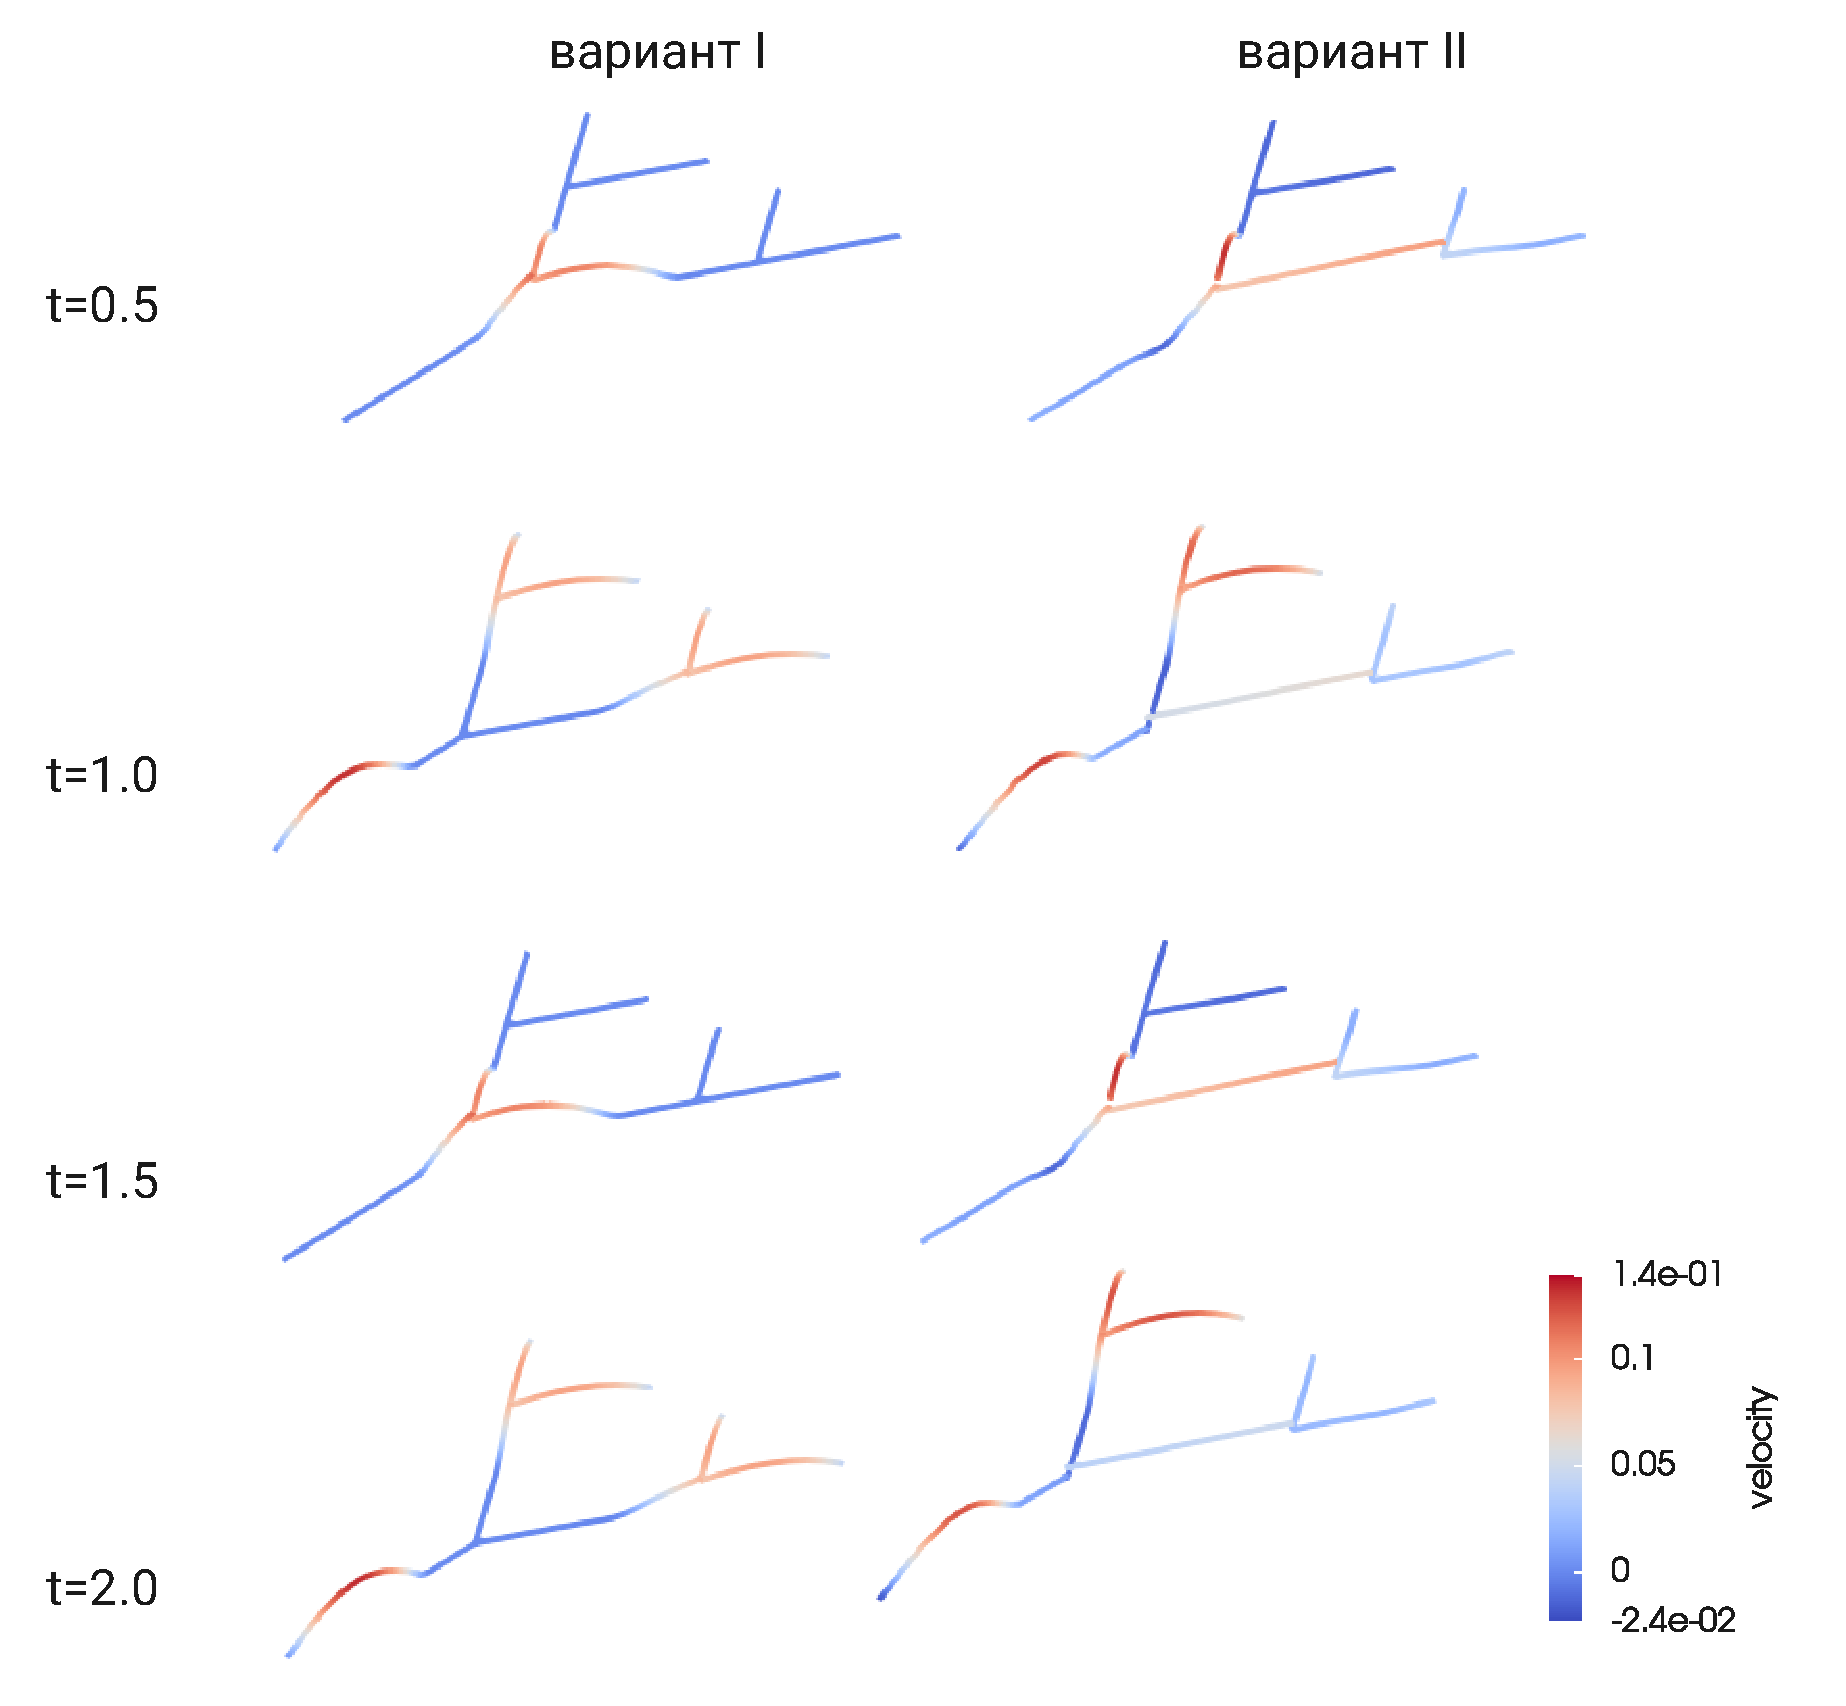
\includegraphics[width=1.0\linewidth]{problem5_time.pdf}
\caption{Значение скорости течения $u$ на различные моменты времени при частоте $bpm=180$. Слева вариант I, справа вариант IV}\label{fig:prob5_time}

\end{figure}

\section{Заключение}
В настоящей работе была рассмотрена нестационарная задача о течении крови в разветвленной сети сосудов с упругими стенками.
Кровь считалась вязкой ньютоновской жидкостью с постоянной плотностью.
Использовалась одномерная модель, в которой определяющие уравнения записываются относительно
средних по сечению сосуда скорости и давления, а также площади этого сечения.
Упругие свойства стенок сосуда описывались по равновесной модели в приближении однородной тонкой эластичной мембраны,
характеризуемой толщиной, модулем упругости и площадью поперечного сечения при отсутствии внешнего воздействия.
Дополнительным упрощением модели являлось использование постоянного радиально-симметричного профиля скорости.

Для определяющей системы уравнений был разработан вычислительный алгоритм. Для аппроксимации по пространству
использовался метод разрывных конечных элементов с Лагранжевыми элементами первого порядка.
Аппроксимация по времени осуществлялась с помощью схемы Кранка--Николсон.
Таким образом, аппроксимации и по времени и по пространству имели второй порядок точности.

Предложенная численная схема была верифицирована путём сравнения её результатов с известными
аналитическими и численными решениями модельных задач о течении крови в аналогичной одномерной постановке.
Рассматривались задачи о течении в одиночном однородном сосуде, о течении в сосуде с неупругой вставкой,
о течении в разветвлении сосудов.
Для всех рассмотренных задач получено удовлетворительное совпадение результатов.

В качестве иллюстрации применения алгоритма для расчёта более сложной системы
была рассмотрена задача течении в сети из семи сосудов,
один из которых имел повышенный модуль упругости и уменьшенный
радиус. Подобные изменения свойств характерны для склеротических поражений сосудов.
Было показано, что наличие таких повреждений в одном из сосудов
ведёт к значительному перераспределению
потоков на выходе из системы сосудов.
Причём разница в значении расходов на выходе из системы
растёт с увеличением частоты сердечных сокращений.


\newpage
\printglossary[type=symbols,style=long3col,title={Условные обозначения}]

\newpage
\printbibliography[heading=bibintoc,title={Список литературы}]

\end{document}
